% !TeX encoding = UTF-8

% 载入 SJTUThesis 模版
\documentclass[degree=bachelor, openany, oneside]{sjtuthesis}
% 选项
%   degree=[doctor|master|bachelor|course],   % 可选(默认:doctor),学位类型
%   zihao=[-4|5],                             % 可选(默认:5),正文字号大小
%   language=[chinese|english],               % 可选(默认:chinese),论文的主要语言
%   review,                                   % 可选(默认:关闭),盲审模式
%   [twoside|oneside]                         % 可选(默认:twoside),单双页模式

% 论文基本配置,加载宏包等全局配置
% !TEX root = ./main.tex

\sjtusetup{
  %
  %******************************
  % 注意:
  %   1. 配置里面不要出现空行
  %   2. 不需要的配置信息可以删除
  %******************************
  %
  % 信息录入
  %
  info = {%
    %
    % 标题
    %   可使用“\\”命令手动控制换行
    %
    title           = {上海交通大学学位论文 \LaTeX{} 模板示例文档},
    title*          = {A Sample Document for \LaTeX-based SJTU Thesis Template},
    %
    % 关键词
    %
    keywords        = {上海交大, 饮水思源, 爱国荣校},
    keywords*       = {SJTU, master thesis, XeTeX/LaTeX template},
    %
    % 姓名
    %
    author          = {某\quad{}某},
    author*         = {Mo Mo},
    %
    % 指导教师
    %
    supervisor      = {某某教授},
    supervisor*     = {Prof. Mou Mou},
    %
    % 副指导教师
    %
    % assisupervisor  = {某某教授},
    % assisupervisor* = {Prof. Uom Uom},
    %
    % 学号
    %
    id              = {0010900990},
    %
    % 学位
    %   本科生不需要填写
    %
    degree          = {工学硕士},
    degree*         = {Master of Engineering},
    %
    % 专业
    %
    major           = {某某专业},
    major*          = {A Very Important Major},
    %
    % 所属院系
    %
    department      = {某某系},
    department*     = {Depart of XXX},
    %
    % 课程名称
    %   仅课程论文适用
    %
    coursename      = {某某课程},
    %
    % 答辩日期
    %   使用 ISO 格式;默认为当前时间
    %
    % date            = {2014-12-17},
    %
    % 资助基金
    %
    % fund  = {
    %           {国家 973 项目 (No. 2025CB000000)},
    %           {国家自然科学基金 (No. 81120250000)},
    %         },
    % fund* = {
    %           {National Basic Research Program of China (Grant No. 2025CB000000)},
    %           {National Natural Science Foundation of China (Grant No. 81120250000)},
    %         },
  },
  %
  % 风格设置
  %
  style = {%
    %
    % 本科论文页眉 logo 颜色
    %   默认为黑色
    %
    % header-logo-color = red,
  },
  %
  % 名称设置
  %
  name = {%
    % publications      = {攻读学位期间完成的论文},
  },
}

% 参考文献支持宏包
\usepackage[backend=biber,style=gb7714-2015,gbpub=false,gbpunctin=false]{biblatex}
% 导入参考文献数据库
\addbibresource{bibdata/thesis.bib}

% 定义图片文件目录与扩展名
\graphicspath{{figures/}}
\DeclareGraphicsExtensions{.pdf,.eps,.png,.jpg,.jpeg}

% 确定浮动对象的位置,可以使用 [H],强制将浮动对象放到这里(可能效果很差)
% \usepackage{float}

% 固定宽度的表格
% \usepackage{tabularx}

% 表格中支持跨行
\usepackage{multirow}

% 表格中数字按小数点对齐
\usepackage{dcolumn}
\newcolumntype{d}[1]{D{.}{.}{#1}}

% 附带脚注的表格
\usepackage{threeparttable}

% 算法环境宏包
\usepackage[ruled,vlined,linesnumbered]{algorithm2e}
% \usepackage{algorithm}

% 代码环境宏包
\usepackage{listings}
\lstnewenvironment{codeblock}[1][]
  {\lstset{style=lstStyleCode,#1}}{}

% 国际单位制宏包
\usepackage{siunitx}

% 定理环境宏包
\usepackage{ntheorem}
% \usepackage{amsthm}

% 绘图宏包
\usepackage{tikz}

% 一些文档中用到的 logo
\usepackage{hologo}
\newcommand{\XeTeX}{\hologo{XeTeX}}
\newcommand{\BibLaTeX}{\textsc{Bib}\LaTeX}

% 借用 ltxdoc 里面的几个命令。
\def\cmd#1{\cs{\expandafter\cmd@to@cs\string#1}}
\def\cmd@to@cs#1#2{\char\number`#2\relax}
\DeclareRobustCommand\cs[1]{\texttt{\char`\\#1}}

\newcommand*{\meta}[1]{{%
  \ensuremath{\langle}\rmfamily\itshape#1\/\ensuremath{\rangle}}}
\providecommand\marg[1]{%
  {\ttfamily\char`\{}\meta{#1}{\ttfamily\char`\}}}
\providecommand\oarg[1]{%
  {\ttfamily[}\meta{#1}{\ttfamily]}}
\providecommand\parg[1]{%
  {\ttfamily(}\meta{#1}{\ttfamily)}}
\providecommand\pkg[1]{{\sffamily#1}}

% 自定义命令

% E-mail
\newcommand{\email}[1]{\href{mailto:#1}{\texttt{#1}}}

% hyperref 宏包在最后调用
\usepackage{hyperref}


\begin{document}

% 无编号内容:中英文论文封面、授权页
\maketitlepage
\makeorigpage*
\makeauthpage[scans/authorization.pdf]

% 使用罗马数字对前言编号
\frontmatter

% 摘要
% !TEX root = ../main.tex

\begin{abstract}
  并发理论是理论计算机科学中一个活跃的研究领域。
  随着大规模通讯系统的迅速发展,
  并发理论成为建模和表征现实并发系统的重要方法论。
  作为经典并发理论的扩展,概率进程被广泛研究,
  产生了很多用于不同的应用场景的各种变体。
  2019年,傅育熙提出了一个对并发进程模型进行概率化扩展的通用方法,
  这一方法具有模型无关性的优点。
  在本文中,我们在这一通用方法的框架下对傅的工作进行了扩展,
  提出了一个传值进程演算的随机版本——随机传值进程模型。
  这一模型是使用傅的通用方法对经典传值进程演算的概率扩展。
  首先,我们规范化了随机传值进程模型的语法和转移语义
  并研究了这一模型的代数性质,例如互模拟关系。
  我们还证明了这一模型等价关系的同余性。
  其次,我们验证了随机传值进程模型可以用于具有传值特点的现实问题的建模和分析。
  作为应用案例,
  我们使用随机传值进程模型有效地建模并模拟实现了基于云计算协议Gossip-Style Membership协议的通信过程,
  证明了随机传值进程模型对于并发通信过程的建模和分析具有一定的可行性。
  我们的工作是傅的通用方法在理论和应用层面上的延伸。
\end{abstract}

\begin{abstract*}
  Concurrency theory has been an active field of research in theoretical computer science.
   Recently, with the rapid development of massive communication systems, 
   concurrency theory has become an important methodology for modeling and characterizing real concurrent systems. 
   As an extension of classic concurrency theory, probabilistic processes have been widely studied for many years and led to lots of variants for different applications. 
   In 2019, Yuxi Fu has proposed a uniform approach to study the probabilistic extension of concurrency processes 
   which has the merit of being model-independent. 
   In this work, we first extend Yuxi’s original work by introducing a random version of value-passing calculus under the uniform approach framework.
  This new model is a randomized extension of the classic value-passing calculus.
   In this paper, we formalize the grammar and transition semantics of the random value-passing calculus, 
   as well as study its algebraic properties such as bisimulation relation. 
   We show that the new equivalence relation is a congruent relation. 
   Second, we show that random value-passing calculus is especially suitable for modeling and analyzing real-world applications with value-passing characteristics. 
   As a case study, we use random value-passing calculus to efficiently model and implement a well-known communication system based on the Gossip-Style Membership Protocol, which is a cloud computing protocol. 
   This shows that our new model is suitable for formalizing and analysis modern concurrent communication systems.
    Our work extends the uniform approach to random process model in both theoretical and application aspects.
\end{abstract*}


% 目录、插图目录、表格目录
\tableofcontents

% \listoffigures*
% \listoftables*
% \listofalgorithms*

% 主要符号、缩略词对照表
% % !TEX root = ../thesis.tex

%TC:ignore

\begin{nomenclature*}
\label{chap:symb}

\begin{longtable}{rl}
  $\epsilon$    & 介电常数 \\  
  $\mu$         & 磁导率 \\
  $\epsilon$    & 介电常数 \\
  $\mu$         & 磁导率 \\
  $\epsilon$    & 介电常数 \\
  $\mu$         & 磁导率 \\
  $\epsilon$    & 电常数 \\
  $\mu$         & 磁导率 \\
  $\epsilon$    & 介电常数 \\
  $\mu$         & 磁导率 \\
  $\epsilon$    & 介电常数 \\
  $\mu$         & 磁导率 \\
  $\epsilon$    & 介电常数 \\
  $\mu$         & 磁导率 \\
  $\epsilon$    & 电常数 \\
  $\mu$         & 磁导率 \\
  $\epsilon$    & 介电常数 \\
  $\mu$         & 磁导率 \\
  $\epsilon$    & 介电常数 \\
  $\mu$         & 磁导率 \\
  $\epsilon$    & 介电常数 \\
  $\mu$         & 磁导率 \\
  $\epsilon$    & 电常数 \\
  $\mu$         & 磁导率 \\
  $\epsilon$    & 介电常数 \\
  $\mu$         & 磁导率 \\
  $\epsilon$    & 介电常数 \\
  $\mu$         & 磁导率 \\
  $\epsilon$    & 介电常数 \\
  $\mu$         & 磁导率 \\
  $\epsilon$    & 电常数 \\
  $\mu$         & 磁导率 \\
  $\epsilon$    & 介电常数 \\
  $\mu$         & 磁导率 \\
  $\epsilon$    & 介电常数 \\
  $\mu$         & 磁导率 \\
  $\epsilon$    & 介电常数 \\
  $\mu$         & 磁导率 \\
  $\epsilon$    & 电常数 \\
  $\mu$         & 磁导率 \\
  $\epsilon$    & 介电常数 \\
  $\mu$         & 磁导率 \\
  $\epsilon$    & 介电常数 \\
  $\mu$         & 磁导率 \\
  $\epsilon$    & 介电常数 \\
  $\mu$         & 磁导率 \\
  $\epsilon$    & 电常数 \\
  $\mu$         & 磁导率 \\
  $\epsilon$    & 介电常数 \\
  $\mu$         & 磁导率 \\
  $\epsilon$    & 介电常数 \\
  $\mu$         & 磁导率 \\
  $\epsilon$    & 介电常数 \\
  $\mu$         & 磁导率 \\
\end{longtable}

\end{nomenclature*}

%TC:endignore


% 使用阿拉伯数字对正文编号
\mainmatter

% 正文内容
% !TEX root = ../main.tex

\chapter{绪论}\label{ch:intro}

并发理论是理论计算机科学中一个活跃的研究领域。
  随着大规模通讯系统的迅速发展,
  并发理论成为建模和表征现实并发系统的重要方法论。
  并发理论的研究内容包括:
  如何刻画并行进程的行为,
  在什么情况下他们可以互相模拟,
  研究各种通信和同步机制和
  死锁、可观察性、发散性等并发现象。
  对并发理论的研究加深了人们对并发系统的认识,
  其主要的研究成果已经在Ada,Java等编程语言中得到广泛应用\cite{计算机科学技术百科全书}。
  在计算机科学中,进程演算(或进程代数)是用于形式化建模并发系统的多种相关方法。
  进程演算提供了具体描述多个独立程序或者是多个进程之间交互、通信、同步的方法,
  其中包含了对进程操作和分析的描述、以及证明形式化推导进程之间存在等价关系的代数法则\cite{History}。
  关于进程演算的典例主要包括
  MILNER R提出的通信系统演算CCS(Calculus of Communicating System)\cite{Milner_CCS},
   HOARE C提出的通信顺序进程CSP(Communicating Sequential Process)\cite{Hoare_CSP},
   BERGSTRA J等提出的ACP(Algebra of Communicating Processes)\cite{BERGSTRA_ACP},
   以及BOLOGNESI T等的LOTOS\cite{LOTOS}。%,Hennessy提出ATPcite{5}等,
   作为描述并发系统的模型,进程演算受到广泛研究并被成功应用到实际系统的规范、设计、分析及验证中。

随机在现代计算机科学的研究中日趋重要,
在对并发系统的研究中也备受关注。
由于现代计算机系统具有开放性、分布式、交互式的特点,
并发系统中通常包含复杂的行为:非确定性行为和随机性行为。
为了使用简单、易用的形式化方法描述复杂的并发系统,
并对并发系统进行建模和分析,
我们通常会使用非确定性行为的统计行为特性。
因此,在并发进程模型中引入随机性的概念是有意义的。
作为经典并发进程模型的重要扩展,
概率进程被广泛研究,
有代表性的工作有对CCS的概率性扩展\cite{CCS_Prob_1,CCS_Prob_2},
概率CSP\cite{CSP_Prob} 和概率ACP\cite{ACP_Prob}等。
近期,FU Y提出了一个通用方法Uniform Approach\cite{Fu_UniformApproach},
可以用于将并发进程模型扩展为概率并发进程模型。
由于其模型无关性,
我们可以使用Uniform Approach对其他并发进程模型进行概率化扩展。

有两种主要的进程演算可以作为概率模型的基础:分别是MILNER R的CCS\cite{Milner_CCS}和HOARE C的CSP\cite{Hoare_CSP}。
它们的区别在与等价的类型和建模并发系统采用的方法\cite{DIFF_CCS_CSP}。
Uniform Approach以CCS为例进行了概率扩展,
为理解Uniform Approach,我们首先对CCS进行简要的介绍。

\section{通信系统演算}

   CCS使用了标记变迁系统(Labled Transition System)来建模。
   CCS的语法如下:
   \begin{equation}
    S,T:=X\mid \sum_{i\in I}\alpha_i.T_i\mid S\mid T \mid (a)T \mid \mu X.T
   \end{equation}

   其中$S,T$为CCS的进程表达式(agent),$X$为进程表达式变元(agent variables)。索引集合$I$是有限自然数集。
   $Chan$为名字(或通道)的集合,其中的元素以小写字母表示,
   集合$\overline{Chan}=\{\overline{a}\mid a\in Chan\}$,
   动作集合$Act=Chan\cup \overline{Chan}\cup \{\tau\} $,
   其中的元素用小写希腊字母表示,$\alpha_i\in Act$,$\tau$表示一切静态迁移(内部动作)。
   $\sum_{i\in I}\alpha_i.T$为非确定性选择项,若$I=\emptyset$,我们可以将这一项写作$0$。
   $S\mid T$表示$S,T$可以并发执行。$(a)T$为限制(Restriction)或内部化(Localization)操作子,对外隐藏$T$中的$a$通道,
   也可以写为$T\backslash \{a\}$或$T\backslash a$。$\mu X$表示递归(Recursion)操作。
   若一个CCS进程表达式$P$中不含自由变元,称$P$为进程(process)。

   CCS的迁移语义如图~\ref{fig_ccs},表示状态之间的变迁规则,其中$\lambda \in Act$。

   \begin{figure}[!htbp]
    \small
    \centering
    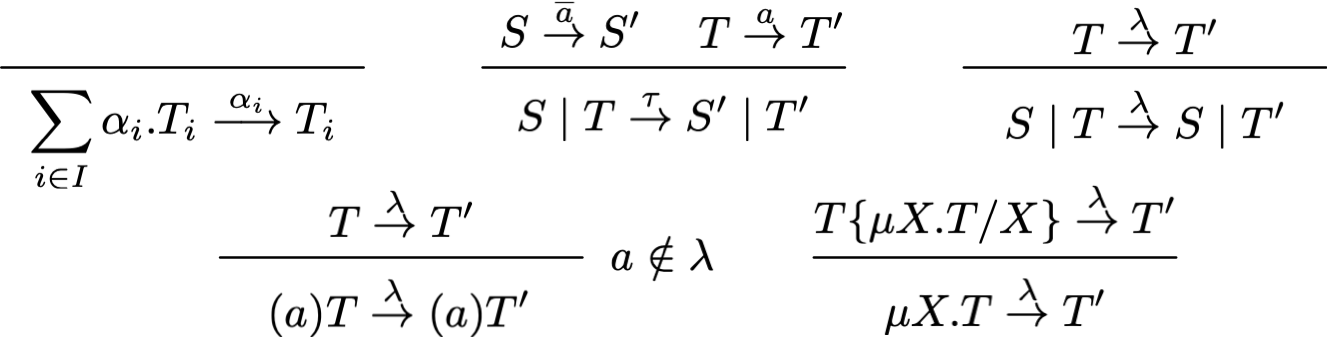
\includegraphics[width=11cm]{../figures/ccs.png}
    \caption[]{\textbf{CCS迁移语义}}
     \label{fig_ccs}
 \end{figure}

   \section{随机进程模型}

   FU Y提供了一个模型无关的方法——An Uniform Approach to Random Process Model(本文中统称为Uniform Approach)\cite{Fu_UniformApproach},
   将进程模型扩展为随机进程模型。
   Uniform Approach区分了非确定性行为和概率性行为,
   在CCS的基础上建立了随机化的CCS(本文中统称为RCCS)的语法、迁移语义并研究了RCCS的代数特性,如互模拟关系。

   RCCS在CCS的基础上增加了概率选择操作子$\bigoplus_{i\in I}p_i\tau.T_i$,
   其中$0<p_i<1 \wedge \sum_{i\in I}p_i = 1$。
   例如,$S=\frac{1}{3}\tau.T_1+\frac{2}{3}\tau.T_2$意味着$S$经过静态迁移(内部动作)变迁为$T_1$状态的概率为$\frac{1}{3}$,
   变迁为$T_2$状态的概率为$\frac{2}{3}$。

   对应随机选择操作子的迁移语义为:
   \begin{figure}[!htbp]
    \small
    \centering
    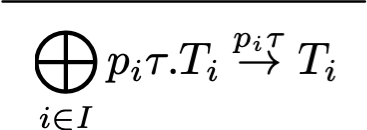
\includegraphics[width=3cm]{../figures/rccs.png}
     \label{fig_rccs}
 \end{figure}

   由于Uniform Approach具有模型无关性,我们可以用它来扩展其他的进程模型,
   进而使非概率模型概率化。

\section{研究目的}
本文希望使用Uniform Approach的通用方法,
概率化扩展经典并发模型——并发传值进程模型,得到随机传值进程模型。
我们可以通过对传值进程模型的扩展,
一方面进一步佐证Uniform Approach的模型无关性;
一方面随机传值进程模型可以应用于具有传值特点的并发系统的建模和分析,
如通信过程、安全协议、生物系统等。
我们希望随机传值进程模型的语法、迁移语义
可以用于为具有传值特点现实问题建模通信、同步等机制,
为这类问题的模型设计与软件开发提供方法,
并可以应用随机传值进程模型的代数特性如互模拟关系、等价关系等
分析模型的死锁、活性、可观察、发散等并发特性。

\section{论文结构}
本文分为四个章节。第\ref{ch:intro}章为绪论,引入了进程演算的概念,
介绍了通信并发演算CCS,引入了一种对进程模型进行概率化扩展的通用方法Uniform Approach。
第\ref{ch:rvpc}章我们使用Uniform Approach中的方法对传值进程模型进行概率化扩展得到随机传值进程模型。
第\ref{ch:gossip}章我们使用随机传值进程模型对基于云计算协议Gossip-Style Membership协议的通信过程建模。
第\ref{ch:conclusion}章为总结以及未来的工作方向。

% !TEX root = ../main.tex

\chapter{随机传值进程模型}\label{ch:rvpc}

由于Uniform Approach是模型无关的概率扩展方法,
我们可以使用该方法概率化扩展其他的进程模型。
本章会对传值进程模型进行概率化扩展。
传值进程模型是经典的进程模型,
在MILNER R的Communication and Concurrency一书\cite{Milner_CCS}中,
也是使用传值的通信并发模型——消息的发送者、接受者和通信媒介——引入并发和通信的概念。
我们选择传值进程模型的一种定义——The Value-Passing Calculus\cite{Fu_VPC}进行扩展。

\section{传值进程模型}
传值进程模型(Value-Passing Calculus)是一种
可以将某个域中的值作为通信的内容,
并且可以在特定逻辑条件执行某个动作的并发进程模型。
一个经典的例子是MILNER R的Communication and Concurrency一书\cite{Milner_CCS}中的一单元缓冲区,它可以接受、储存、发送消息:
\begin{equation}
   \begin{split}
      C&\stackrel{def}{=}in(x).C'(x)\\
   C'(x)&\stackrel{def}{=}\overline{out}(x).C
   \end{split}
\end{equation}
其中CCS进程表达式$C$接受了$in$通道输入的变元$x$的一个值时会变迁为$C'(x)$状态,$C'(x)$通过$\overline{out}$通道输出$x$的值时会变迁为$C$。

更普遍的传值进程模型也可以对输入进行逻辑判定,
根据特定的条件执行特定的动作,
通过输入控制进程的执行。我们以进程$A(x)$为例:
\begin{equation}
   A(x)=\textrm{if }\varphi(x)\textrm{ then }\overline{a}(f(t))\textrm{ else }B(x)
\end{equation}
$A(x)$在满足条件$\varphi(x)$时会通过通道$a$输出函数$f(t)$的值,
其中$t$可能是$x$的函数,也可能与$x$无关;若不满足$\varphi(x)$,则执行程序$B(x)$。

传值进程模型赋予了进程传递数据的能力,
我们可以通过进程之间传递的数据来控制进程的执行和进程间的交互,
这种控制能力显著的增强了并发进程模型的表达能力,
拓宽了并发进程模型的应用场景。
在网络通信中,各种通信协议通过在主机间传值进而控制主机的行为,
执行通信协议的通信系统就可以被抽象为并发传值进程模型,
支持并发的编程语言也可以被解释为传值进程模型,如Erlang\cite{Erlang}。
很多通过传值、计算解决的现实问题也都可以抽象为传值进程模型。


\subsection{The Value-Passing Calculus}\label{ch:vpc}
对传值进程模型的研究很多都会依赖一个\textit{神域},
这个神域是一个领域模型(domain model)或一个逻辑理论(logic theory),
帮助我们进行条件的判定,函数的计算和提供变元的取值范围。
如在执行$A(x)$时,我们会将$\varphi(x)$传给神域,
神域判定是否满足条件,并将判定结果返回给我们,
同样的,我们也会将$f(t)$传给神域,神域帮我们计算这个函数,并将结果返回给我们。
例如,WINSKEL G等人将变元表达式的取值和计算全部依赖一个集合$V$\cite{Oracle_V},
LIN H等人依赖一个评估$\rho$完成布尔表达式的判定和表达式的计算\cite{Oracle_rho},
其中最经典的并发传值模型是MILNER R对CCS的扩展Value-Passing CCS\cite{Milner_CCS},
上述两个传值进程模型也是基于Value-Passing CCS。 
MILNER R的Value-Passing CCS在CCS中引入了带数据参数的动作和进程,
使它比之CCS刻画实际系统的能力大大提升,Value-Passing CCS中有下列数据类型:
$Val$表示数据值的集合其元素用$v$表示,相似的$x\in DVar$为数据变量,
$e\in DExp$为数据表达式,$b\in BExp$为布尔表达式,$\rho$为$DVal$到$Val$的全映射,
与CCS相同$a,c\in Chan$。
Value-Passing CCS的语法可以表示为:
\begin{equation}
   S,T:=0|A(e)|\sum_{i\in I}\alpha_i.T|S|T|(a)T|if\;b\;then\;T
\end{equation}
其中$\alpha:=\tau|c(x)|\overline{c}(t)$,$t$或是$\rho(x)$计算所得或与$x$无关,
$A(e)$为进程常量\cite{VPCCS}。
然而MILNER R在Value-Passing CCS的定义过程中没有讨论函数的计算过程和$if\;b\;then\;T$中条件$b$的可判定性,
可以认为MILNER R的传值进程模型同样依赖神域帮助Value-Passing CCS完成这些未定义的工作。

神域通常不包括在传值进程模型中,且通常是未定义的,或只在特定场景下定义。
由于神域的存在,对于这些传值进程模型表达能力的衡量变得十分困难,
FU Y在The Value-Passing Calculus中取缔了神域的概念,
提出了一个封闭的传值进程模型\cite{Fu_VPC},这个模型同时也是不针对某一应用场景的通用模型。

The Value-Passing Calculus中的传值进程模型$\mathbb{VPC}_{\mathsf{Th}}$
的语法可以表示为:
\begin{equation}\label{eq:vpc}
   T:=\sum_{i\in I}\varphi_i a(x).T_i|\sum_{i\in I}\varphi_i\overline{a}(t_i).T_i|T|T'|(c)T|\varphi T|!a(x).T|!\overline{a}(t).T
\end{equation}
其中$T$是一个$\mathbb{VPC}_{\mathsf{Th}}$项,$\mathsf{Th}$是可判定的逻辑,
$\varphi_i$是一个布尔表达式,可以通过$\mathsf{Th}$证明或证伪,
若$\mathsf{Th}$可以给出$\varphi_i$的一个证明,记为$\mathsf{Th}\vdash \varphi_i$。
$a(x)$是一个输入前缀,$\overline{a}(t_i)$是一个输出前缀,
我们可以用$\sum_{i\in I}\varphi_i\lambda_i.T_i$来表示$\sum_{i\in I}\varphi_i a(x).T_i$或$\sum_{i\in I}\varphi_i \overline{a}(t).T_i$。
$!a(x).T$和$!\overline{a}(t).T$对应递归操作,$\mu X.E$可以表示为
$(c)(E\{c(z).0/X\}|!\overline{c}(r).E\{c(z).0/X\})$。
其余的表达与第一章CCS语法定义的解释相同。

The Value-Passing Calculus提出了两种迁移语义的描述:具体语义(Concrete Semantics)和符号语义(Symbolic Semantics)。
后文我们只用到了符号语义,因此我们忽略具体语义的相关内容。

$\mathbb{VPC}_{\mathsf{Th}}$的符号迁移语义如图~\ref{fig_vpc}所示。

\begin{figure}[!htbp]
   \small
   \centering
   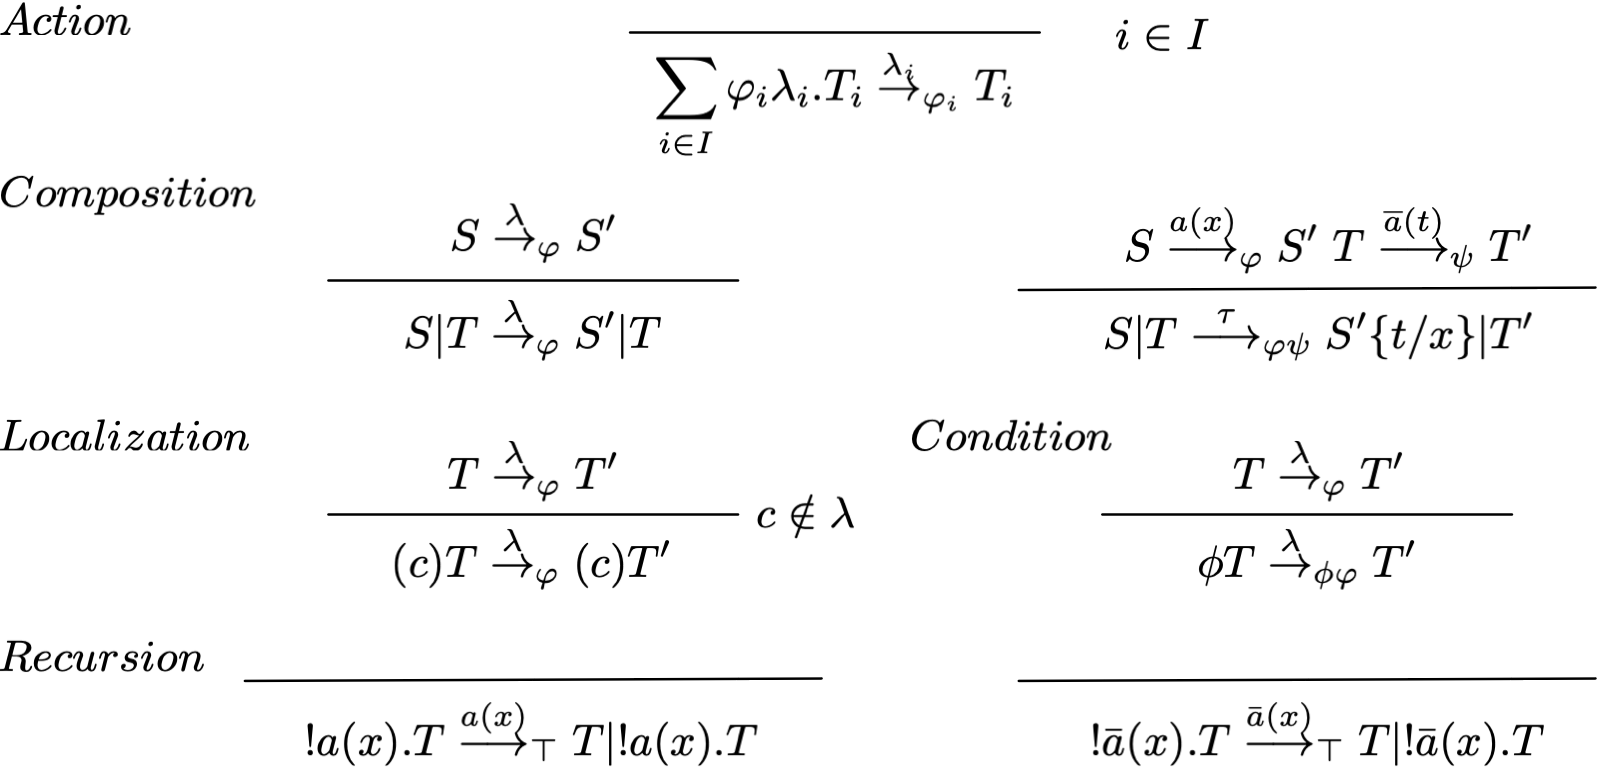
\includegraphics[width=13cm]{../figures/vpc.png}
    \caption[]{$\mathbb{VPC}_{\mathsf{Th}}$的符号迁移语义规则}
    \label{fig_vpc}
\end{figure}
其中,$T=\varphi \lambda.T'$在$\varphi$条件下执行$\lambda$动作到达$T'$状态,
在符号语义下可以写作$T\stackrel{\lambda}{\rightarrow}_{\varphi}T'$。
符号语义中的动作集合$Act=\{a(x),\overline{a}(t)| a\in Chan, x\in \mathsf{V}_{\Sigma}, t\in \mathsf{T}_{\Sigma}\}\cup \{\tau\}$,
$Act$中的元素可以用$\lambda$表示,其中$\mathsf{V}_{\Sigma},\mathsf{T}_{\Sigma}$为可判定逻辑$\mathsf{Th}$中变元的集合和项的集合\cite{Fu_VPC}。

The Value-Passing Calculus使用可判定的一阶理论判定条件\cite{PA}并
提出了一个图灵完备的数值系统(Numeric System)\cite{Fu_VPC}作为底层模型来实现可计算的函数。
通过这两种方式,将Value-Passing Calculus从神域中解放出来。

\subsection{If Then Else语法符号化}
进程$A(x)$中出现了If Then Else语法,
If Then Else语法实现的分支控制在编程中也是非常重要的组成部分。
在Communication and Concurrency\cite{Milner_CCS}中也多次使用If Then Else语法,
然而在CCS的定义中,我们无法通过CCS进程表达式的语法规则来实现这种分支控制;
书中对分支控制的使用,如第五章(Bisimulation and Observation Equivalence)中对JobShop的建模\cite{Milner_CCS}
也比较随意,没有严格的定义也没有判断If条件的可判定性。
在FU Y的The Value-Passing Calculus\cite{Fu_VPC}中,
规定了If条件是通过一阶理论$\mathsf{Th}$可判定的布尔表达式,
并说明$\textrm{if }\varphi\textrm{ then }S\textrm{ else }T$
可以被定义为$\varphi S|\urcorner \varphi T$。
以下推论依据The Value-Passing Calculus中对If Then Else语法的定义和$\mathbb{VPC}_{\mathsf{Th}}$的Proof System,
给出If Then Else的变体的符号化定义,在本文的后续章节会统一使用这些符号。

以下推论中$S,T\in \mathcal{T}_{\mathbb{VPC}_\mathsf{Th}}$。
\begin{corollary} 
   $\varphi 0 = 0$
\end{corollary}
\begin{proof}
   $\varphi 0 = \varphi 0 + 0 = \varphi 0 + \top 0 = \varphi 0 + (\varphi \vee \urcorner \varphi)0 = \varphi 0 + \varphi 0 + \urcorner \varphi 0 = \varphi 0 + \urcorner \varphi 0 = (\varphi \vee \urcorner \varphi)0 = \top 0 = 0$
\end{proof}
\begin{corollary}
   $\varphi T = (\varphi T\mid \urcorner \varphi 0)$
\end{corollary}
\begin{proof}
   $\varphi T = (\varphi T\mid 0) = (\varphi T\mid \urcorner \varphi 0)$
\end{proof}
\begin{corollary}
   $S=\urcorner\varphi \varphi T$,则$S=0$。
\end{corollary}
\begin{proof}
   $S=\urcorner\varphi \varphi T = (\urcorner\varphi\wedge\varphi)T=\bot T=0$
\end{proof}
进而我们可以得到If Then Else语法与$\mathbb{VPC}_\mathsf{Th}$规则的对照表:
\begin{table}[!hpt]
   \caption{\textbf{If Then Else语法对照表}}
   \label{tab:ifthenelse}
   \centering
   \begin{tabular}{@{}cc@{}} \toprule
   %   \multicolumn{2}{c}{Item} \\ \cmidrule(r){1-2}
     语法 & $\mathbb{VPC}_{\mathsf{Th}}$规则对照 \\ \midrule
     $S=$ if $\varphi$ then $T$ else $T'$& $S=(\varphi T|\urcorner \varphi T')$\\
     $S=$ if $\varphi$ then $T$ & $S=(\varphi T|\urcorner\varphi 0)$\\
     $S = $if $\urcorner \varphi$ then if $\varphi$ then $T$ & $S=0$\\ \bottomrule
   \end{tabular}
 \end{table}
\section{随机传值进程模型}
由于随机性的可计算性,
许多具有传值性质的通信过程、生物分析等现实问题的建模和分析也被引入了概率的思想,如SWIM协议\cite{SWIM}和生物自组装系统\cite{BioProcess}。
我们可以在传值进程模型中引入随机性用于对这些具有随机性、传值特点的问题,或者可以用概率分布近似表示非确定性行为的系统进行建模和分析。
目前已经存在使用随机传值进程模型建模和分析网络安全\cite{NetworkSecurity}等应用,
但由于其是在Value-passing CCS\cite{Milner_CCS}基础上的概率扩展,
以\cite{NetworkSecurity,Prob_VPCCS}为例的模型仍然存在神域的问题。

为了避免神域带来的问题,我们可以将随机传值进程模型定义在$\mathbb{VPC}_{\mathsf{Th}}$的基础上,
用Uniform Approach中的随机选择$\bigoplus_{i\in I}p_i\tau.T_i$
扩展公式~\ref{eq:vpc}中$\mathbb{VPC}_{\mathsf{Th}}$项的定义。
我们可以得到随机传值进程模型(Random VPC,记为$\mathbb{RVPC}_{\mathsf{Th}}$)项的定义:
\begin{equation}\label{eq:rvpc}
   T:=\bigoplus_{i\in I}p_i \tau.T_i\mid \sum_{i\in I} \varphi_i\lambda_i.T_i\mid T \mid T'\mid (c)T\mid \varphi T\mid !a(x).T \mid !\bar{a}(t).T
\end{equation}
其中,与~\ref{ch:vpc}中定义的一样:$\lambda_i \in Act$,$\mathsf{Th}$为可判定的一阶理论。
随机选择操作子$\bigoplus_{i\in I}p_i\tau.T_i$中,$0<p_i<1, \sum_{i\in I}p_i = 1$。
$S=\bigoplus_{i\in I}p_i\tau.T_i$意味着$S$在$p_i$的概率下经过内部动作$\tau$到达$T_i$状态。

$\mathcal{T}_{\mathbb{RVPC}_{\mathsf{Th}}}$为所有$\mathbb{RVPC}_\mathsf{Th}$的项$T$的集合。

在~\ref{ch:vpc}中$\mathbb{VPC}_{\mathsf{Th}}$的符号语义的基础上,
增加\label{fig_rccs}定义的随机选择操作子的迁移规则,
我们可以得到随机传值进程模型的符号语义,
其中随机选择的条件为$\top$,
表明该操作在任意条件下可执行;
若随机选择也需要在特定条件下执行,
我们可以配合$\mathbb{VPC}_{\mathsf{Th}}$中的条件操作子,
得到$\varphi (\bigoplus_{i\in I}p_i\tau.T_i)$。

\begin{figure}[!htbp]
	\small
	\centering
	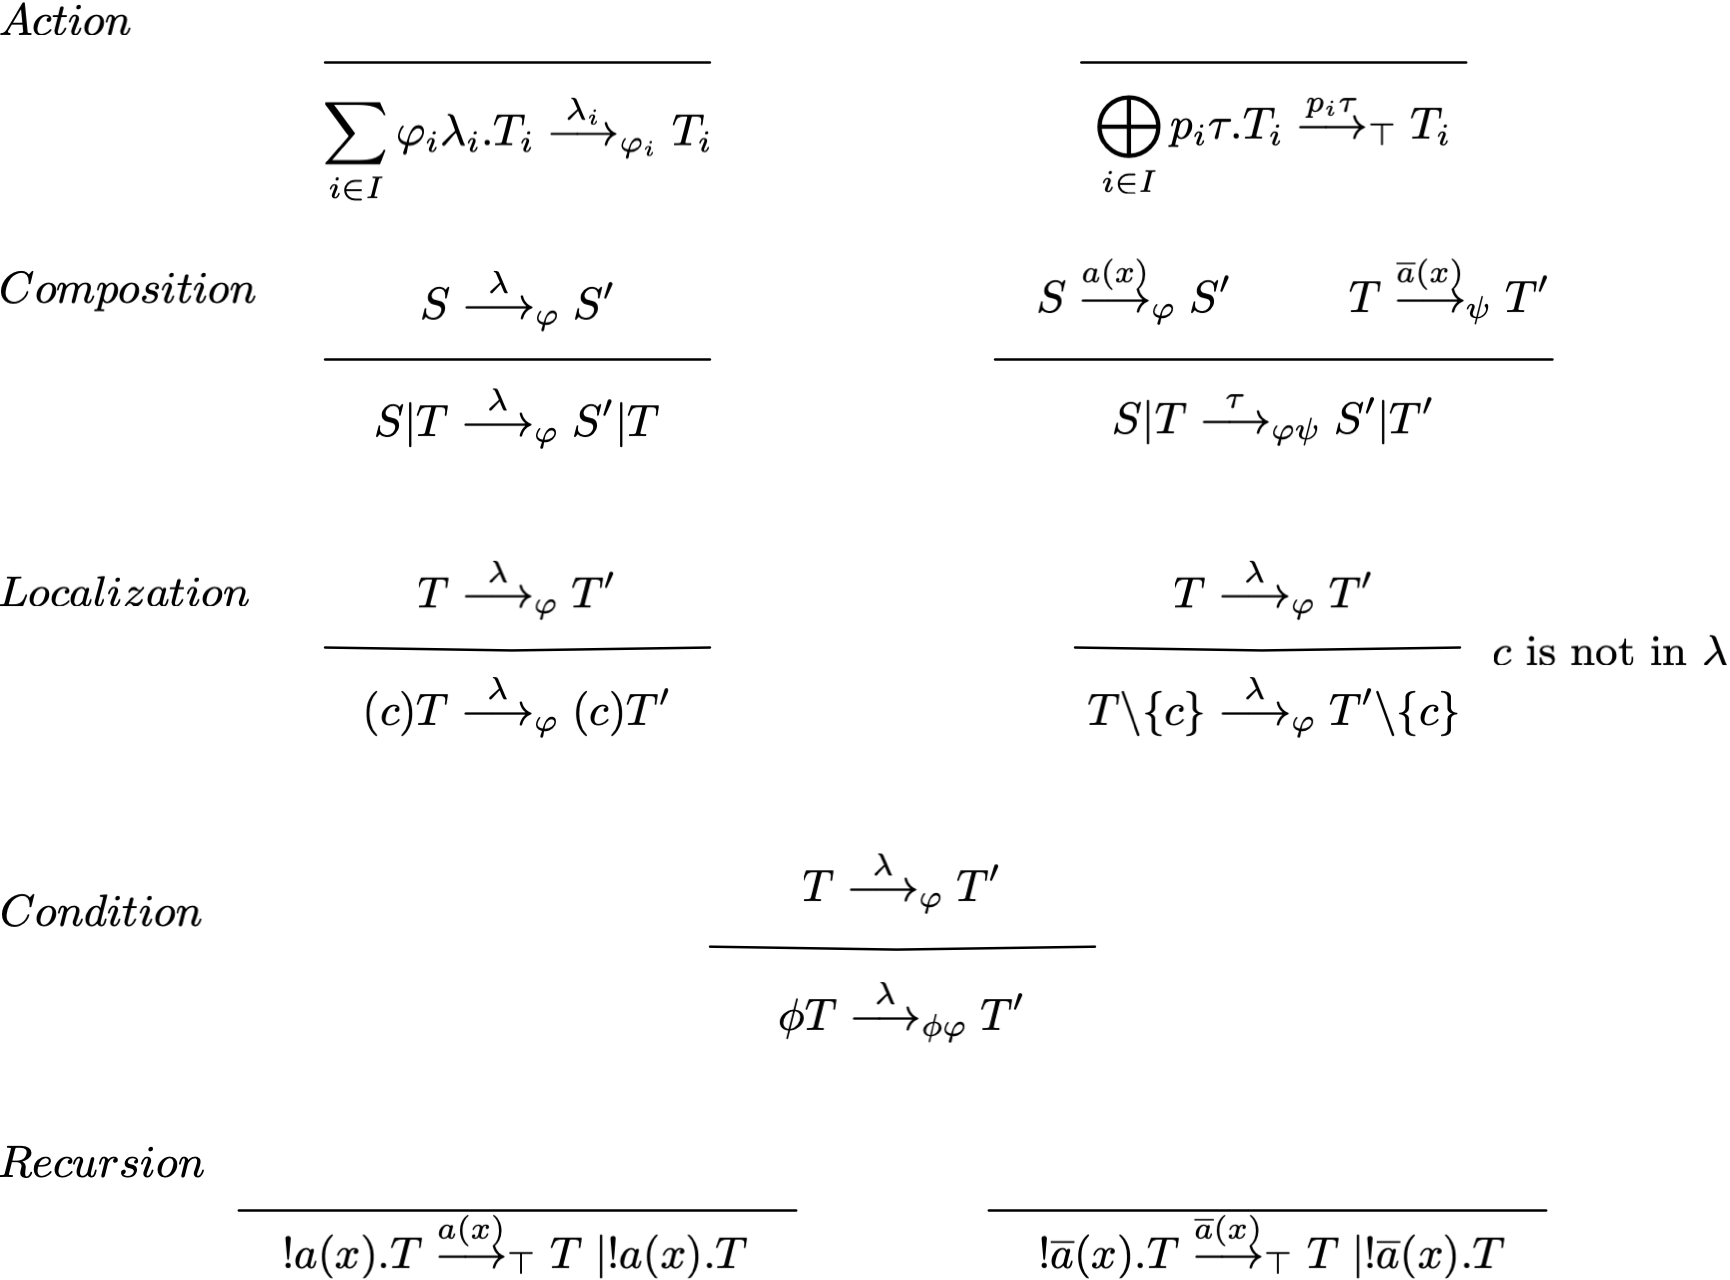
\includegraphics[width=14cm]{../figures/symbolic_sematic.png}
    \caption{随机传值进程模型的符号迁移语义}
    \label{fig_sematic}
\end{figure}

对于$\mathbb{VPC}_{\mathsf{Th}}$的前缀操作子的迁移规则:
$\sum_{i\in I} \varphi_i \lambda_i. T_i\stackrel{\lambda_i}{\rightarrow}_{\varphi_i} T_i$,
它本质上代表了非确定选择,
即作出$\varphi_i$条件下的$\lambda_i$动作到达$T_i$状态是非确定的,
我们可以通过Uniform Approach的方法将它扩展为一个概率性选择,
即在概率$p_i$下会作出$\varphi_i$条件下的$\lambda_i$动作:
$\bigoplus_{i\in I} p_i\tau.\varphi_i \lambda_i. T_i\stackrel{p_i\tau}{\rightarrow}_{\top}\stackrel{\lambda_i}{\rightarrow}_{\varphi_i} T_i$。
它的语义为:在概率$p_i$下,我们会经过一个内部$\tau$操作到达一个$\mathbb{RVPC}_{\mathsf{Th}}$状态:
$\varphi_i\lambda_i.T_i$,
若$\mathsf{Th}\vdash \varphi_i$(即一阶理论$\mathsf{Th}$下,$\varphi_i$为真),
则我们可以经过$\lambda_i$操作到达$\mathbb{RVPC}_{\mathsf{Th}}$状态$T_i$, 
其中$\lambda_i \in \{a(x),\bar{a}(x)\mid a\in Chan, x\in \mathsf{V}_\Sigma, t\in \mathsf{T}_\Sigma\}\cup \{\tau\}$。

$\mathbb{RVPC}_{\mathsf{Th}}$在$\mathbb{VPC}_{\mathsf{Th}}$的基础上扩展了前缀操作:$p\tau.$,
其中$p\in (0,1)$。
类似$A=\tau.B$的$\mathbb{RVPC}_{\mathsf{Th}}$项,
我们可以认为$A\stackrel{1\tau}{\rightarrow}_{\top} B$,
这时也满足$A=\bigoplus_{i\in I} p_i\tau.A_i$的定义,
此时$I=\{1\},p_1=1,A_1=B$。
若将$\mathbb{VPC}_{\mathsf{Th}}$中的此类内部操作同样看待,
我们可以得出推论~\ref{co:vpc}。
\begin{corollary}\label{co:vpc}
   $\mathbb{VPC}_{\mathsf{Th}}$是一种特殊的$\mathbb{RVPC}_{\mathsf{Th}}$。
\end{corollary}

\section{随机传值进程模型中的互模拟关系}

\subsection{互模拟关系与观察等价性}\label{ch:bisimulation}

   程序理论的基本问题是进程的等价性。
   等价关系的定义为:设$R$是非空集合$A$上的二元关系,
   若$R$是自反的、对称的、传递的,则称$R$是$A$上的等价关系。
   研究等价关系的目的在于将集合中的元素进行分类,选取每类的代表元素来降低问题的复杂度,如软件测试时,可利用等价类来选择测试用例\cite{Equiv}。
   对通信并发系统程序等价的定义和验证,现在已有很多研究。
   互模拟等价性为进程描述语言提供了有效的语义理论。
   在提出CCS时MILNER R提出了\textit{观察等价(observation equivalence)}与\textit{弱互模拟(weak bisimulation)}\cite{Milner_CCS}。
   Van GLABBEEK R和WEIJLAND W提出的\textit{分支互模拟(branching bisimulation)}\cite{Branching_1, Branching_2}也是十分著名的研究。

   对于概率模型的等价性,目前有对全概率进程模型,即概率选择代替非确定性选择的进程模型的弱互模拟及分支互模拟的研究\cite{全概率的弱互模拟和分支互模拟},
   仅适用于有限状态的概率进程模型的研究\cite{有限状态_1,有限状态_2}等。
   Uniform Approach在分支互模拟\cite{Branching_1, Branching_2}的基础上给出了
   RCCS分支互模拟关系的定义,以及等价关系同余性的证明。
   
   RCCS的分支互模拟是CCS分支互模拟的扩展,我们首先来看CCS的分支互模拟。
   $\mathcal{P}_{CCS}$上的分支互模拟的定义如下:
   \begin{definition}\label{def:branching0}
      $\mathcal{E}$是在$\mathcal{P}_{CCS}$上的对称关系,若对于任意$A,B\in \mathcal{P}_{CCS},A\mathcal{E}B$满足:

            若$A\stackrel{l}{\rightarrow}A'$,则$l=\tau$且$A'\mathcal{E}B$或存在$B',B''$使得
            $B\stackrel{\tau}{\rightarrow}\dots\stackrel{\tau}{\rightarrow}B'\stackrel{l}{\rightarrow}B''$且$A\mathcal{E}B'\wedge A'\mathcal{E}B''$。

            则称$\mathcal{E}$是在$\mathcal{P}_{CCS}$上一个分支互模拟关系。
   \end{definition}
   
   内部操作$\tau$带来的状态迁移可以称为\textit{静态迁移}。
   若$\sim$是$\mathcal{P}_{CCS}$上的一个等价关系,
   当$A\stackrel{\tau}{\rightarrow}A'\sim A$时,
   我们可以写为$A\stackrel{\tau}{\rightarrow}_{\sim}A'$,
   当$A\stackrel{\tau}{\rightarrow}\dots \stackrel{\tau}{\rightarrow}A'\sim A$时,
   我们可以写为$A\stackrel{\tau}{\Rightarrow}_{\sim}A'$。
   在Uniform Approach中,这种动作称为\textit{状态保持的静态迁移(state-preserving silent transition)},
   对应的,若$A\stackrel{\tau}{\rightarrow}\dots \stackrel{\tau}{\rightarrow}A'\not\sim A$,
   称为\textit{状态改变的静态迁移(state-changing silent transition)}。
   $\Rightarrow_{\sim}$为$\stackrel{\tau}{\rightarrow}_{\sim}$的闭包。

   Uniform Approach中RCCS的分支互模拟涉及等价集的概念,我们首先看$\mathcal{P}_{CCS}$上的等价集的定义:
   \begin{definition}
      若二元关系$\mathcal{E}$是$\mathcal{P}_{CCS}$上的等价关系。
      $A$关于等价关系$\mathcal{E}$的等价集写作$[A]_{\mathcal{E}}$,
      $A\in [A]_{\mathcal{E}}$,若$(A,B)\in \mathcal{E}$,
      有$B\in [A]_{\mathcal{E}}$。
      我们用$\mathcal{P}_{CCS}/\mathcal{E}$表示所有$\mathcal{P}_{CCS}$关于$\mathcal{E}$的等价集的集合。
   \end{definition}
   $\mathcal{P}_{RCCS}$,$\mathcal{T}_{\mathbb{VPC}_{\mathsf{Th}}}$,$\mathcal{T}_{\mathbb{RVPC}_{\mathsf{Th}}}$上的等价集的定义都是相似的,因此不做赘述。

      引入了等价集的概念后,我们可以将分支互模拟的形式简化为定义~\ref{def:branching}的形式:
   \begin{definition}\label{def:branching}
      $\mathcal{E}$是$\mathcal{P}_{CCS}$上的等价关系,
      若对于任意动作$l,l\neq \tau$和任意等价集$\mathcal{C}\in \mathcal{P}_{CCS}/\mathcal{E}, \mathcal{C}\neq [A]_{\mathcal{E}}$,
      满足若$B\mathcal{E}A\Rightarrow_{\mathcal{E}}\stackrel{l}{\rightarrow}\mathcal{C}$,则$B\Rightarrow_{\mathcal{E}}\stackrel{l}{\rightarrow}\mathcal{C}$,
      称$\mathcal{E}$是$\mathcal{P}_{CCS}$上的分支互模拟关系。
   \end{definition}
   定义~\ref{def:branching}与定义~\ref{def:branching0}虽然本质上是相同的,
   但是定义~\ref{def:branching}更好的揭示了分支互模拟的核心思想:
   一系列状态保持的静态模拟后的状态改变的静态迁移之间的相互模拟。

   考虑到RCCS在CCS的基础上增加了概率选择,
   状态保持的静态迁移在$A\stackrel{\tau}{\rightarrow}A'\mathcal{E}A$的基础上新增了
   $A\stackrel{p\tau}{\rightarrow} A'\mathcal{E}A,0<p<1$的可能,
   为了用类似$\Rightarrow_{\mathcal{E}}$的方式表示这种静态迁移,
   Uniform Approach提出了\textit{等价树(Epsilon Tree)}的概念\cite{Fu_UniformApproach},
   将概率选择作为树的分支,节点$A$的关于等价关系$\mathcal{E}$的等价树上的任意节点$N\in [A]_{\mathcal{E}}$。
   同时,Uniform Approach定义了两种迁移:$l$-迁移($l$-transition)和$q$-迁移($q$-transition),
   分别表示等价树上的节点迁移到其他等价集动作和概率,Uniform Approach中定义的概率版分支互模拟是对$l$-迁移和$q$-迁移的相互模拟。

   \begin{definition}[$l$-迁移($l$-transition)]
      $A\in \mathcal{P}_{RCCS}$,
      从$A$到$\mathcal{B}\in \mathcal{P}_{RCCS}/\mathcal{E},\mathcal{B}\neq [A]_{\mathcal{E}}$的
      $l$-迁移表示$A$关于等价关系$\mathcal{E}$的等价树上的每一个叶子结点$L$,
      存在$L\stackrel{l}{\rightarrow}L'\in\mathcal{B},l\neq \tau$,写作$A\rightsquigarrow_{\mathcal{E}}\stackrel{l}{\rightarrow}\mathcal{B}$。
   \end{definition}

   \begin{definition}[$q$-迁移($q$-transition)]
      $A\in \mathcal{P}_{RCCS}$,$\mathcal{E}$为$\mathcal{P}_{RCCS}$上的等价关系,
      $L$为$A$关于等价关系$\mathcal{E}$的等价树上的每一个叶子结点,
      $\mathcal{B}\in \mathcal{P}_{RCCS}/\mathcal{E}, \mathcal{B}\neq [A]_{\mathcal{E}}$。

      定义$\mathsf{P}(L\stackrel{\coprod_{i\in[k]}p_i\tau}{\longrightarrow}\mathcal{B})=\sum \{p_i|L\stackrel{p_i\tau}{\longrightarrow}L_i\in \mathcal{B}\wedge i\in I\}$。
      
      定义$\mathsf{P}_{\mathcal{E}}(L\stackrel{\coprod_{i\in[k]}p_i\tau}{\longrightarrow}\mathcal{B})=\mathsf{P}(L\stackrel{\coprod_{i\in[k]}p_i\tau}{\longrightarrow}\mathcal{B})/(1-\mathsf{P}(L\stackrel{\coprod_{i\in[k]}p_i\tau}{\longrightarrow}[A]_{\mathcal{E}}))$。

      当$\mathsf{P}_{\mathcal{E}}(L\stackrel{\coprod_{i\in[k]}p_i\tau}{\longrightarrow}\mathcal{B})=q$时,
      记为$A\rightsquigarrow_{\mathcal{E}}\stackrel{q}{\rightarrow}\mathcal{B}$,即$q$-迁移。
   \end{definition}

   现在我们终于可以引入Uniform Approach中定义的RCCS的分支互模拟关系了!

   \begin{definition}
      当$\mathcal{P}_{RCCS}$上的等价关系$\mathcal{E}$满足:
      \begin{itemize}
         \item[(1)] {
            若$B\mathcal{E}A\rightsquigarrow_{\mathcal{E}}\stackrel{l}{\rightarrow}\mathcal{C}\in \mathcal{P}_{RCCS}/\mathcal{E}, l\neq \tau \wedge \mathcal{C}\neq [A]_{\mathcal{E}}$,则$B\rightsquigarrow_{\mathcal{E}}\stackrel{l}{\rightarrow}\mathcal{C}$。
         }
         \item[(2)] {
            若$B\mathcal{E}A\rightsquigarrow_{\mathcal{E}}\stackrel{q}{\rightarrow}\mathcal{C}\in \mathcal{P}_{RCCS}/\mathcal{E}, l\neq \tau \wedge \mathcal{C}\neq [A]_{\mathcal{E}}$,则$B\rightsquigarrow_{\mathcal{E}}\stackrel{q}{\rightarrow}\mathcal{C}$。
         }
      \end{itemize}
      则等价关系$\mathcal{E}$是分支互模拟关系。
   \end{definition}

   $\mathbb{VPC}_{\mathsf{Th}}$与CCS的区别主要体现在前缀操作子和条件操作子,
   这也是传值的进程模型与非传值的进程模型的主要区别。
   对于前缀操作子,相似的定义互模拟关系是比较容易的,只需要保证通道一致、值一致即可。
   而条件操作子给互模拟的定义带来了麻烦,比如:
   $A=\overline{a}(0).S$和$B=((x=0) \overline{a}(0).S|\urcorner (x=0) \overline{a}(0).S)$在观察上应该是一致的,
   但若我们应用分支互模拟$A$可以作出$A\stackrel{a(0)}{\rightarrow}_{\top}S$的动作,
   而$B$不能。
   但对于$A\stackrel{a(0)}{\rightarrow}_{x=0}S$和$A\stackrel{a(0)}{\rightarrow}_{\urcorner (x=0)}S$,
   $B$却可以相应的作出模拟的动作。
   这就要求$B$的两个操作:$B\stackrel{\overline{a}(0)}{\longrightarrow}_{x=0} S$和$B\stackrel{\overline{a}(0)}{\longrightarrow}_{\urcorner (x=0)} S$共同模拟$A\stackrel{\overline{a}(0)}{\longrightarrow}_{\top} S$。

   为了上述问题HENNESSY M和LIN H为传值进程模型提出了符号迁移图(Symbolic Transition Graph)和符号互模拟(Symbolic Bisimulation)的概念\cite{Symbolic_bisimulation}。
   在The Value-Passing Calculus中,FU Y也提出了$\mathbb{VPC}_\mathsf{Th}$的符号互模拟\cite{Fu_VPC}。
   
   \begin{definition}[符号互模拟]\label{def:symbolic_bisimulation}
      $\mathcal{E}$是一个$\mathcal{T}_{\mathbb{VPC}_{\mathsf{Th}}}$上的二元对称关系,
      当$A\mathcal{E}B$满足下列条件时,称$\mathcal{E}$是一个符号互模拟关系:
      \begin{itemize}
         \item[(1)] {
            若$A\stackrel{\tau}{\rightarrow}_{\varphi} A'$,则存在$\varphi$的划分$\{\varphi_i\}_{i\in I}$和集合$\{B\Rightarrow_{\psi_i} B_i\}_{i\in I}$,
            对于$\forall i\in I$,$\mathsf{Th}\vdash \varphi_i\Rightarrow \psi_i\wedge \varphi_i A\mathcal{E} \varphi_i B_i$,
            且满足$\varphi_i A'\mathcal{E} \varphi_i B_i$或$B_i\stackrel{\tau}{\rightarrow}_{\psi_i'}B_i'\wedge \mathsf{Th}\vdash \varphi_i\Rightarrow \psi_i'\wedge \varphi_i A'\mathcal{E} \varphi_i B_i'$。
         }
         \item[(2)] {
            若$A\stackrel{\overline{a}(t)}{\rightarrow}_{\varphi} A'$,则存在$\varphi$的划分$\{\varphi_i\}_{i\in I}$和集合$\{B\Rightarrow_{\psi_i}B_i\stackrel{\overline{a}(t_i)}{\rightarrow}_{\psi_i'}B_i'\}$,
            满足$\mathsf{Th}\vdash (\varphi_i\Rightarrow \psi_i\psi_i')\wedge (\varphi_i \Rightarrow t=t_i)$且$(\varphi_i A\mathcal{E}\varphi_i B_i)\wedge(\varphi_i A'\mathcal{E}\varphi_i B_i')$。
         }
         \item[(3)] {
            若$A\stackrel{a(x)}{\rightarrow}_{\varphi} A'$,则存在$\varphi$的划分$\{\varphi_i\}_{i\in I}$和集合$\{B\Rightarrow_{\psi_i}B_i\stackrel{a(x)}{\rightarrow}_{\psi_i'}B_i'\}$,
            满足$\mathsf{Th}\vdash \varphi_i\Rightarrow \psi_i\psi_i'$且$(\varphi_i A\mathcal{E}\varphi_i B_i)\wedge(\varphi_i A'\mathcal{E}\varphi_i B_i')$。
         }
      \end{itemize}
      互模拟关系的全集记为$\approxeq_{\mathsf{Th}}^s$。
   \end{definition}

   根据符号互模拟的定义,我们可以解决前述条件操作子带来的麻烦,
   我们可以通过下面的例子验证这一点。
   \begin{example}
      证明$A=\overline{a}(0).S$和$B=((x=0) \overline{a}(0).S|\urcorner (x=0) \overline{a}(0).S)$是符号互模拟的。
   \end{example}
   \begin{proof}
      定义等价关系$\mathcal{E}=\{(A,B)\}\cup \equiv$,
      其中$\equiv$为绝对等价关系,
      题目等价于证明$\mathcal{E}$是一个符号互模拟关系。

      对于$A\stackrel{\overline{a}(0)}{\rightarrow}_{\top} S$,
      存在$\top$的划分$\{(x=0),\urcorner(x=0)\}$和集合
      $\{B\stackrel{\overline{a}(0)}{\longrightarrow}_{x=0}S, B\stackrel{\overline{a}(0)}{\longrightarrow}_{\urcorner(x=0)}S\}$,
      且$(x=0)S\mathcal{E}(x=0)S$。

      对于$B\stackrel{\overline{a}(0)}{\longrightarrow}_{x=0}S$,存在$A\stackrel{\overline{a}(0)}{\longrightarrow}_{x=0}S$与之符号互模拟。
      $B\stackrel{\overline{a}(0)}{\longrightarrow}_{\urcorner(x=0)}S$同理。
   \end{proof}

   \subsection{条件等价树}

   根据~\ref{ch:bisimulation}中定义~\ref{def:symbolic_bisimulation}中定义的$\mathbb{VPC}_{\mathsf{Th}}$的符号互模拟关系,
   我们观察$A(x)=(x\geq 5)\overline{a}(\mathsf{s}(x)).0)$和$A'(x)=(x\geq 3)\overline{a}(\mathsf{s}(x)).0$,
   根据$\mathbb{VPC}_\mathsf{Th}$的符号互模拟的定义,我们容易得到$A$和$A'$是不符号互模拟的,
   对于$A'(t)\stackrel{\overline{a}(\mathsf{s}(t))}{\longrightarrow}_{x\geq 3} 0$,
   因为$3<x<5$的这一部分动作是$A(x)$无法完成的,所以不存在$x\geq 3$的划分,
   使得$A(x)$可以给出一个迁移的集合来模拟整个$x\geq 3$。
   但反观$B(x)=(x>5)A(x),B'(x)=(x>5)A'(x)$,
   我们可以得到$B'(x)=((x>5)\wedge(x\geq 3))\overline{a}(\mathsf{s}(x)).0=(x>5)\overline{a}(\mathsf{s}(x)).0$,
   同理$B(x)=(x>5)\overline{a}(\mathsf{s}(x)).0$,
   $B(x),B'(x)$不仅是符号互模拟,甚至是绝对等价的。
   对于$(x>5)A(x)$和$(x>5)A'(x)$的这种关系,
   我们给出\textit{条件等价集}的定义,可以使等价集内部对某个条件透明:

   \begin{definition}[条件等价集]
     $A,A'\in \mathcal{T}_{\mathbb{RVPC}_{\mathsf{Th}}}$,$\mathcal{E}$是$\mathbb{RVPC}_{\mathsf{Th}}$上的等价关系,
     若$\varphi A \mathcal{E} \varphi A'$,则$A'\in [A]_{\varphi \mathcal{E}}$。
     $[A]_{\varphi \mathcal{E}}$称为等价关系$\mathcal{E}$在条件$\varphi$下包含$A$的等价集。 
     我们用$\mathcal{T}_{\mathbb{RVPC}_{\mathsf{Th}}}/\varphi \mathcal{E}$表示所有$\mathbb{RVPC}_{\mathsf{Th}}$关于布尔表达式$\varphi$和等价关系$\mathcal{E}$的条件等价集的集合。 
   \end{definition} 

   由于$\mathbb{VPC}_{\mathsf{Th}}$是特殊的$\mathbb{RVPC}_{\mathsf{Th}}$,
   条件等价集的定义同样适用$\mathbb{VPC}_{\mathsf{Th}}$。
   显然,$A'(x)\in [A(x)]_{(x>5)\mathcal{E}}$,其中$\mathcal{E}=\approxeq_{\mathsf{Th}}^s$。
   
   条件$\top$具有一定的特殊性:
   对于无条件的操作我们认为操作是在$\top$条件下执行的,
   因此$\top$可以看作是最强的条件。
   \begin{corollary}\label{co:condition0}
      $A,B\in \mathcal{T}_{\mathbb{VPC}_{\mathsf{Th}}}$,
      若$A\approxeq_{\mathsf{Th}}^s B$,
      则对布尔表达式$\varphi$,
      $\varphi A\approxeq_{\mathsf{Th}}^s\varphi B$。
   \end{corollary}
   \begin{proof}
      对于$A$可以执行的操作,$\varphi' A$也会有对应的版本:
      \begin{itemize}
         \item[(1)] 若$A\stackrel{\tau}{\rightarrow}_{\varphi} A'$,则$\varphi' A\stackrel{\tau}{\rightarrow}_{\varphi' \varphi}A'$。
         \item[(2)] 若$A\stackrel{a(x)}{\rightarrow}_{\varphi} A'$,则$\varphi' A\stackrel{a(x)}{\rightarrow}_{\varphi' \varphi} A'$。
         \item[(3)] 若$A\stackrel{\overline{a}(t)}{\rightarrow}_{\varphi} A'$,则$\varphi' A\stackrel{\overline{a}(t)}{\rightarrow}_{\varphi' \varphi} A'$。
      \end{itemize}
      对$\varphi' A\stackrel{a(x)}{\rightarrow}_{\varphi'\varphi} A'$,
      根据$A\approxeq_{\mathsf{Th}}^sB$,我们知道存在$\varphi$的划分$\{\varphi_i\}_{i\in I}$和集合$\{B\Rightarrow_{\psi_i}B_i\stackrel{a(x)}{\rightarrow}_{\psi_i'}B_i'\}_{i\in I}$,
      满足$\mathsf{Th}\vdash \varphi_i\Rightarrow \psi_i \psi_i' \wedge \varphi_i A\approxeq_{\mathsf{Th}}^s \varphi_i B_i \wedge \varphi_i A'\approxeq_{\mathsf{Th}}^s \varphi_i B_i'$。
      
      若要证明$\varphi' A\approxeq_{\mathsf{Th}}^s\varphi' B$,
      我们可以构造等价关系$\mathcal{S} = \{(\varphi'A,\varphi'B)|(A,B)\in \approxeq_{\mathsf{Th}}^s\}$,
      证明$\mathcal{S}$是符号互模拟的,其中$A,B$为任意$\mathcal{T}_{\mathbb{VPC}_{\mathsf{Th}}}$。

      通过$A\approxeq_{\mathsf{Th}}^sB$我们可以得到集合$\{\varphi'\varphi_i\}_{i\in I}$,
      对于任意$i,j$,由于$\varphi_i \wedge \varphi_j = \bot$,
      我们可以得到$(\varphi'\varphi_i) \wedge (\varphi'\varphi_j) = \bot$;
      又$\bigvee_{i\in I}\varphi_i = \varphi$,$\bigvee_{i\in I}\varphi'\varphi_i = \varphi'\varphi$,
      因此$\{\varphi'\varphi_i\}_{i\in I}$为$\varphi'\varphi$的划分。
      我们还可以得到集合$\{\varphi'B\Rightarrow_{\varphi'\psi_i}B_i\stackrel{a(x)}{\rightarrow}_{\psi_i'} B_i'\}$,
      满足$\mathsf{Th}\vdash \varphi'\varphi_i\Rightarrow \varphi'\psi_i\psi_i'$,
      而$(\varphi'\varphi_i A, \varphi'\varphi_i B_i),(\varphi'\varphi_i A', \varphi'\varphi_i B_i')\in \mathcal{S}$,
      因此我们可以用$\{\varphi'B\Rightarrow_{\varphi'\psi_i}B_i\stackrel{a(x)}{\rightarrow}_{\psi_i'} B_i'\}$模拟$\varphi' A\stackrel{a(x)}{\rightarrow}_{\varphi'\varphi} A'$。

      对称的一边和其他两种情况的证明是相似的。
   \end{proof}

   \begin{corollary}\label{co:all}
      $A,B\in \mathbb{RVPC}_{\mathsf{Th}}$,$\mathcal{E}$是$\mathbb{RVPC}_{\mathsf{Th}}$上的等价关系,
      $\varphi$是任意布尔表达式,
      若$B\in [A]_{\mathcal{E}}$,则$B\in [A]_{\varphi \mathcal{E}}$。
   \end{corollary}
   
   推论~\ref{co:all}可以简单理解为:一个$\mathbb{RVPC}_{\mathsf{Th}}$项在任意条件下成立的等价集是所有条件等价集的交集。
   我们也可以给出一个简单的证明。
   \begin{proof}
      $A,B\in \mathcal{T}_{\mathbb{RVPC}_{\mathsf{Th}}}$,
      $fv(\varphi)$为$\varphi$中的自由变元的集合,
      $V$为$fv(\varphi)$的全部取值的集合,
      对于$fv(\varphi)$的每一个赋值$v\in V$,
      我们可以得到一个无自由变元的布尔表达式$\varphi_v$:
      \begin{itemize}
         \item[(1)] {
            若$\mathsf{Th}\vdash \varphi_v$,$\varphi_vA=A\mathcal{E}B=\varphi_v B$。
         }
         \item[(2)] {
            若$\mathsf{Th}\not\vdash \varphi_v$,$\varphi_v A=0=\varphi_v B$。
         }
      \end{itemize}
   \end{proof}

   将$\top$推广到其他布尔表达式,我们可以得到更为广泛的结论:

   \begin{corollary}\label{co:condition}
      $A,B\in \mathcal{T}_{\mathbb{VPC}_{\mathsf{Th}}}$,
      若$\varphi A\approxeq_{\mathsf{Th}}^s \varphi B$,
      则对布尔表达式$\varphi',\mathsf{Th}\vdash \varphi'\Rightarrow \varphi$,
      $\varphi' A\approxeq_{\mathsf{Th}}^s\varphi' B$。
   \end{corollary}

   \begin{corollary}\label{co:all_1}
      $A,B\in \mathbb{RVPC}_{\mathsf{Th}}$,$\mathcal{E}$是$\mathbb{RVPC}_{\mathsf{Th}}$上的等价关系,
      $\varphi$是任意布尔表达式,
      若$B\in [A]_{\varphi\mathcal{E}}$,
      则对于布尔表达式$\varphi',\mathsf{Th}\vdash\varphi'\Rightarrow \varphi$,
      $B\in [A]_{\varphi' \mathcal{E}}$。
   \end{corollary}

   \begin{corollary}\label{co:superset}
      $L\in \mathcal{T}_{\mathbb{RVPC}_{\mathsf{Th}}}$,
      $L$关于布尔表达式$\varphi$和等价关系$\mathcal{E}$的等价集为$\mathcal{C}=[L]_{\varphi\mathcal{E}}$,
      对任意$\mathsf{Th}\vdash \varphi'\Rightarrow\varphi$,
      $L$关于$\varphi'\mathcal{E}$的等价集$[L]_{\varphi'\mathcal{E}}$是$\mathcal{C}$的超集,
      可以将$[L]_{\varphi'\mathcal{E}}$记为$[\mathcal{C}]_{\varphi'\mathcal{E}}$。
   \end{corollary}
   推论~\ref{co:superset}可以由推论~\ref{co:all_1}得出。

   定义~\ref{def:symbolic_bisimulation}给出了$\mathbb{VPC}_{\mathsf{Th}}$的互模拟的定义,
   观察定义~\ref{def:symbolic_bisimulation}中的$A\stackrel{a(x)}{\longrightarrow}_{\varphi} A'$,
   我们用$\{B\Rightarrow_{\psi_i}B'_i\stackrel{a(x)}{\longrightarrow}_{\psi'_i}B_i'\}$模拟,
   其中$(\varphi_i A\mathcal{E}\varphi_i B_i)\wedge(\varphi_i A'\mathcal{E}\varphi_i B_i')$,
   根据条件等价集的定义,我们可以得到$B_i\in [A]_{\varphi\mathcal{E}}$,$B_i'\in [A']_{\varphi \mathcal{E}}$,
   由于$B_i \approxeq_{\mathsf{Th}}^s A$,$B_i\approxeq_{\mathsf{Th}}^s B$,那么$B\Rightarrow_{\psi_i}B_i\in[B]_{\varphi\mathcal{E}}$实际上也是\textit{状态保持的静态迁移}。

   对于我们概率扩展后的$\mathbb{RVPC}_{\mathsf{Th}}$,
   对上述例子状态保持静态迁移多了$B\stackrel{q\tau}{\rightarrow}_{\psi_i} B_i$
   的情况,其中$q\in(0,1)$,表示\textit{概率的状态保持的静态迁移}。
   我们希望可以找到$\mathbb{RVPC}_{\mathsf{Th}}$中类似$\Rightarrow_{\mathcal{E}}$的方式来表达这种状态保持的静态迁移。
   我们可以使用Uniform Approach中等价树的方法来刻画这种状态保持的静态迁移,
   在$\mathbb{RVPC}_{\mathsf{Th}}$中称为\textit{条件等价树}。

   在定义条件等价树之前,我们首先关注一种条件无关的静态迁移树:
\begin{definition}[静态迁移树]
   \label{def:silent_tree}
   若$A\in \mathcal{T}_{\mathbb{RVPC}_{\mathsf{Th}}}$,
   $A$的静态迁移树$t$满足如下定义:
   \begin{itemize}
   \item[(1)] 每一个节点都被标记成$\mathcal{T}_{\mathbb{RVPC}_{\mathsf{Th}}}$的一个项,$A$是根节点。
   \item[(2)] {
      节点间的边被标记成$(\varphi,p)$,其中$p\in(0,1]$,$\varphi$是一个布尔表达式。
      如果一条从$A'$到$A''$的有向边被标记成$(\varphi,p)$,表示$A'\stackrel{p\tau}{\rightarrow}_{\varphi} A''$。
   }
   \end{itemize}
\end{definition}

静态迁移树包含了\textit{状态改变的静态迁移}和\textit{状态保持的静态迁移},
条件等价树需要对特定条件下的状态改变的静态迁移进行剪枝:

\begin{definition}[条件等价树]
   $\varphi$是一个布尔表达式,$\mathcal{E}$是$\mathcal{T}_{\mathbb{RVPC}_{\mathsf{Th}}}$上的等价关系,
   $A\in \mathcal{T}_{\mathbb{RVPC}_{\mathsf{Th}}}$,
   当下列条件成立时,$A$的静态迁移树$t$称为是一个关于$\varphi\mathcal{E}$的条件等价树($\varphi \mathcal{E}$-tree) ,记作$t^A_{\varphi \mathcal{E}}$。
\begin{itemize}
   \item[(1)] $t$上的所有节点$N$,$N\in [A]_{\varphi \mathcal{E}}$,并被重新标记为$\varphi N$。
   \item[(2)] {
   若$t$的边被标记为$(\psi, q)$,则$\mathsf{Th}\vdash \varphi\Rightarrow \psi$。
   }
   \item[(3)] {
         若$B,B'$是$t$上的节点,
         $B\stackrel{(\psi,q)}{\rightarrow}B',q\in (0,1)$,
         则存在$B\stackrel{\coprod_{i\in [k]}}{\longrightarrow}_{\psi} \coprod_{i\in [k]} B_i$,
         $B_i,i\in [k]$是$t$上的节点,
         且$B$有且仅有$B_1,\dots, B_k$这$k$个儿子节点,
         且根据(2),有$\mathsf{Th}\vdash \varphi\Rightarrow \psi$。
   }
   \item[(4)] {
      若$B,B'$是$t$上的节点,
      $B\stackrel{(\psi,1)}{\rightarrow}B'$,
      则有$B\stackrel{\tau}{\rightarrow}_{\psi}B'$且$B$有且仅有$B'$一个儿子节点,
      且根据(2),有$\mathsf{Th}\vdash \varphi\Rightarrow \psi$。
   }
\end{itemize}
\end{definition}

条件等价树实质上是\textit{概率的状态保持的静态迁移}。

从定义上看条件等价树的定义比较抽象,我们可以看几个简单有趣的例子:

\begin{example}\label{eg:conditional}
   $A(x)=(x>5)(\frac{1}{2}\tau.B(x)\oplus\frac{1}{2}\tau.C(x))|(x\leq 5)(\frac{1}{3}\tau.B(x)\oplus\frac{2}{3}\tau.C(x))$。
   若$[A(x)]_{\mathcal{E}}=[B(x)]_{\mathcal{E}}=[C(x)]_{\mathcal{E}}$,
   我们可以得到$A(x)$的静态迁移树如图\ref{fig:eg_condition},$A(x)$关于$(x>7)\mathcal{E}$的条件等价树如图\ref{fig:eg_condition2}。

\begin{figure}[!htp]
   \begin{minipage}{0.6\textwidth}
   \centering
   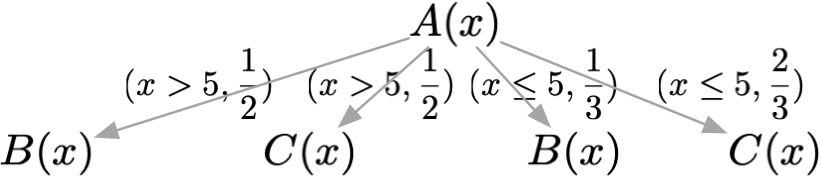
\includegraphics[width=8cm]{../figures/example_condition.png}
   \caption{$A(x)$的静态迁移树}
  \label{fig:eg_condition}
\end{minipage}\hfill
\begin{minipage}{0.45\textwidth}
   \centering
   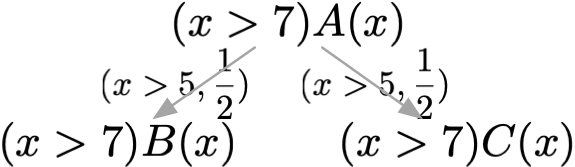
\includegraphics[width=5cm]{../figures/example_condition2.png}
   \caption{$A(x)$关于$(x>7)\mathcal{E}$的条件等价树}
   \label{fig:eg_condition2}
\end{minipage}
 \end{figure}
\end{example}
\begin{example}
   $H(x)\stackrel{def}{=}(x\leq 3)(\frac{1}{3}\tau.(x\leq 1)G(x)\oplus\frac{1}{3}\tau.(x\leq 2)G(x)\oplus\frac{1}{3}\tau.(x\leq 3)G(x))$

   $[H(x)]_{\mathcal{E}_1} = [G(x)]_{\mathcal{E}_1}$,$H(x),G(x)\in \mathbb{RVPC}_{\mathsf{Th}}$,其中$\mathsf{Th}=\mathsf{PA}$\cite{PA}。

   $H(x)$的静态迁移树如图~\ref{fig_eg0_1},它包含了$H(x)$所有的静态迁移。
   \begin{figure}[!htp]
      \begin{minipage}{0.6\textwidth}
         \centering
         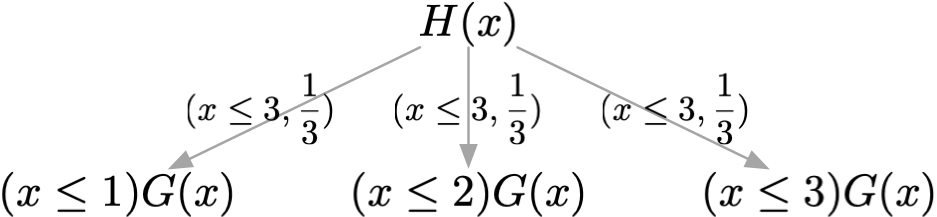
\includegraphics[width=8cm]{../figures/example0_1.png}
         \caption[]{$H(x)$的静态迁移树}
         \label{fig_eg0_1}
   \end{minipage}\hfill
   \begin{minipage}{0.45\textwidth}
      \centering
      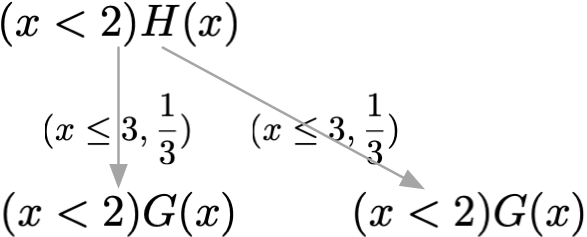
\includegraphics[width=5cm]{../figures/example0_2.png}
      \caption[]{$H(x)$的$(x<2)\mathcal{E}_1$条件等价树}
       \label{fig_eg0_2}
   \end{minipage}
    \end{figure}

   因为$\mathsf{Th}\vdash \top \not\Rightarrow (x\leq 3)$,
   $H(x)$的$\top\mathcal{E}_1$-tree只有一个根节点$H(x)$。

   同理,$H(x)$的$(x>3)\mathcal{E}_1$-tree只有一个根节点$H(x)$。

   $H(x)$的$(x<2)\mathcal{E}_1$条件等价树如图~\ref{fig_eg0_2},
   其中$\mathsf{Th}\vdash (x<2)\Rightarrow (x\leq 3)$,
   由于$(x<2)\wedge(x\leq 2)G(x) = (x<2)G(x)$,$G(x)\in[H(x)]_{\mathcal{E}_1}$,
   根据推论~\ref{co:all},$(x\leq 2)G(x)\in [H(x)]_{(x<2)\mathcal{E}_1}$。
   另一个分支同理。此时实际有$(x<2)H(x)\stackrel{\frac{2}{3}\tau}{\rightarrow}_{\top}[(x<2)G(x)]_{(x<2)\mathcal{E_1}}$,
   因此在条件树内部,我们可以将节点和边都视为状态无关。

\end{example}
\begin{example}\label{eg:1}
      假设我们有一个不太行的下课铃系统,每一时刻它坏掉的可能性是$\frac{1}{2}$,可以通过内部自动校准系统(静态迁移:$\tau$操作)修复,
      它的内部有一个计时器,每隔定长时间($\tau$操作)就会从$a$通道广播录好的一段下课铃,
      录好的下课铃可以用变元$x$表示。
      这个下课铃系统可以被抽象为一个$\mathbb{RVPC}_{\mathsf{Th}}$,其中$\mathsf{Th}$可以认为是$\mathsf{PA}$\cite{PA},
      我们可以用$G(x)$来表示这个系统:
      \begin{equation}
         G(x)\stackrel{def}{=}\mu X.(\frac{1}{2}\tau.X\oplus \frac{1}{2}\tau.\overline{a}(x).X)
      \end{equation}
      $G(x)$在$\mathcal{E}_2$的等价集$[G(x)]_{\top\mathcal{E}_2} = [\overline{a}(x).G(x)]_{\top\mathcal{E}_2}$。
      $G(x)$的$\top \mathcal{E}_2$条件等价树如图~\ref{fig_eg1}。
      \begin{figure}[!htbp]
         \small
         \centering
         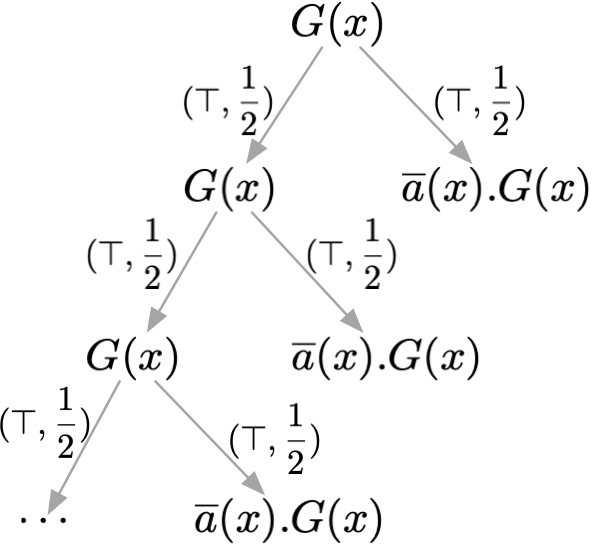
\includegraphics[width=5cm]{../figures/example1.png}
         \caption[]{$G(x)$的$\top \mathcal{E}_2$条件等价树} 
         \label{fig_eg1}
      \end{figure}
\end{example}
\begin{example}\label{eg:2}
   假设例~\ref{eg:1}的下课铃系统经过岁月的磨练,年久失修,
   每自动校准一次音量就会减弱,我们用变元$y$来表示音量,
   音量必须满足$y>1$才可以播放,
   当$y\leq 0$时下课铃系统音量就无法减弱了。
   为了方便建模,我们用$\mathsf{p}(x)=x-1$来表示这种音量减弱。
   校长出于节约经费的考虑,只要下课铃还能在他办公室听见($y>3$)就可以继续使用,
   现在的下课铃系统依然是一个$\mathbb{RVPC}_{\mathsf{Th}}$,
   我们可以用修改的$G'(x,y)$来表示这个系统:
   \begin{equation}
      G'(x,y)\stackrel{def}{=}(y>3)(\frac{1}{2}\tau.((y>0)\tau.G'(x,\mathsf{p}(y))|\urcorner (y>0)\tau.G'(x,y))\oplus \frac{1}{2}\tau.((y>1)\overline{a}(x).G'(x,y)))
   \end{equation}
   $G'(x,y)$在$(y>3)\mathcal{E}_3$的等价集$[G'(x,y)]_{(y>3)\mathcal{E_3}}=[G'(x,y')]_{(y'>3)\mathcal{E_3}}=[\overline{a}(x).G'(x,y'')]_{(y''>3)\mathcal{E_3}}$,其中$y,y',y''$不一定相等。

   $G'(x,y)$的$(y>3)\mathcal{E}_3$条件等价树如图~\ref{fig_eg2}。
   \begin{figure}[!htbp]
      \small
      \centering
      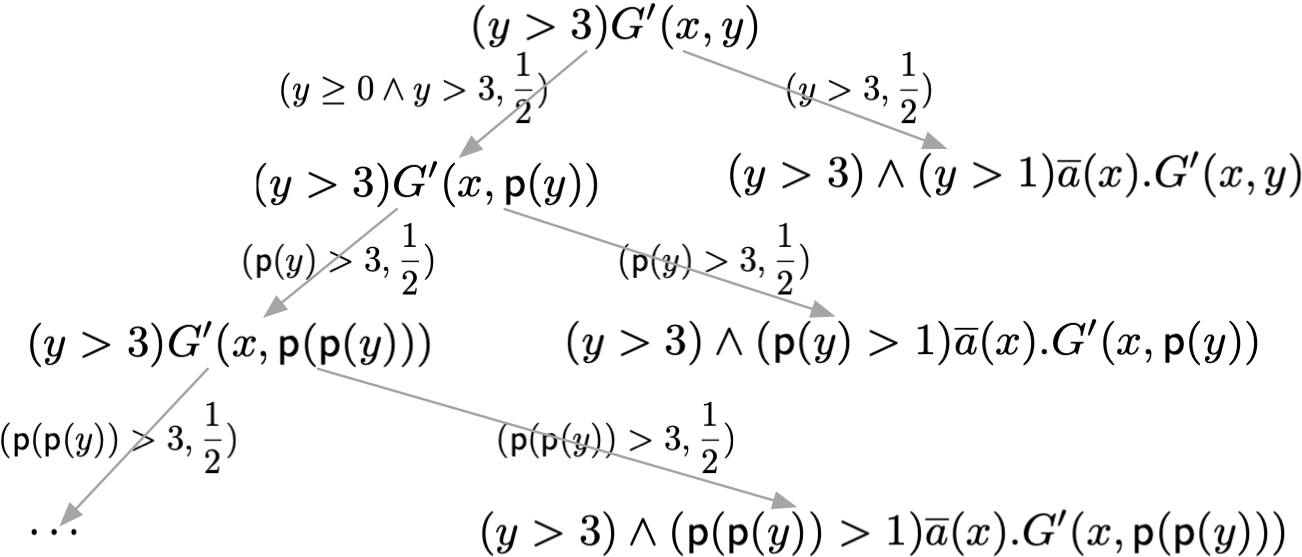
\includegraphics[width=11cm]{../figures/example2.png}
      \caption[]{$G'(x,y)$的$(y>3)\mathcal{E}_3$条件等价树} 
      \label{fig_eg2}
   \end{figure}
   其中$\mathsf{p}(x)$的实现可以通过FU Y的The Value-Passing Calculus中的Numeric System\cite{Fu_VPC}实现。
\end{example}

\subsection{随机传值进程模型的符号互模拟}\label{ch:symbolic_bisimulation}
定义了\textit{概率的状态保持的静态迁移},
我们现在可以用Uniform Approach的方法得到$\mathbb{RVPC}_{\mathsf{Th}}$的符号互模拟。
我们首先需要定义随机传值进程模型条件版的$l$-迁移和$q$-迁移。

\begin{definition}[条件$l$-迁移($\varphi l$-transition)]
   $A\in \mathcal{T}_{\mathbb{RVPC}_{\mathsf{Th}}}, \mathcal{B}\in \mathcal{T}_{\mathbb{RVPC}_{\mathsf{Th}}}/\varphi'\mathcal{E}\backslash [A]_{\varphi'\mathcal{E}}$,
   其中$\varphi'$是一个布尔表达式,$\mathcal{E}$是$\mathcal{T}_{\mathbb{RVPC}_{\mathsf{Th}}}$上的等价关系,
   若$A$的条件等价树$t_{\varphi' \mathcal{E}}^A$的所有叶子结点$L$,
   存在$L\stackrel{l}{\rightarrow}_{\varphi} L'\in \mathcal{B},l\neq \tau$,
   称为$\varphi'$条件下$A$到$\mathcal{B}$的$\varphi l$-迁移,记作$A\rightsquigarrow_{\varphi'\mathcal{E}}\stackrel{l}{\rightarrow}_{\varphi}\mathcal{B}$。
\end{definition}

\begin{definition}[条件$q$-迁移($\varphi q$-transition)]
   $A\in \mathcal{T}_{\mathbb{RVPC}_{\mathsf{Th}}},\mathcal{B}\in (\mathcal{T}_{\mathbb{RVPC}_{\mathsf{Th}}}/\varphi' \mathcal{E})\backslash [A]_{\varphi'\mathcal{E}}$,
   其中$\varphi'$是一个布尔表达式,$\mathcal{E}$是$\mathcal{T}_{\mathbb{RVPC}_{\mathsf{Th}}}$上的等价关系,
   对$t^A_{\varphi' \mathcal{E}}$的每一个叶子结点$L$和布尔表达式$\varphi$,
   若$L\stackrel{\coprod_{i\in I}p_i\tau}{\longrightarrow}_{\coprod_{i\in I}\psi_i} \coprod_{i\in [k]}L_i$,
$i\in I, L_i\in \mathcal{B}$,且$\mathsf{Th}\vdash \varphi \Rightarrow \psi_i$:

定义$\mathsf{P}_\varphi(L\stackrel{\coprod_{i\in I}p_i\tau}{\longrightarrow}_{\coprod_{i\in I}\psi_i}\mathcal{B}) = \sum\{p_i\mid L\stackrel{p_i\tau}{\rightarrow}_{\psi_i} L_i\in\mathcal{B} \wedge i\in I \wedge \mathsf{Th}\vdash \varphi \Rightarrow \psi_i\}$。

定义$\mathsf{P}_{\varphi, \varphi' \mathcal{E}}(L\stackrel{\coprod_{i\in I}p_i\tau}{\longrightarrow}_{\coprod_{i\in I}\psi_i}\mathcal{B}) = \mathsf{P}_\varphi(L\stackrel{\coprod_{i\in I}p_i\tau}{\longrightarrow}_{\coprod_{i\in I}\psi_i}\mathcal{B})/(1-\mathsf{P}_\varphi(L\stackrel{\coprod_{i\in I}p_i\tau}{\longrightarrow}_{\coprod_{i\in I}\psi_i}[A]_{\varphi\mathcal{E}}))$。

当$\mathsf{P}_{\varphi,\varphi' \mathcal{E}}(L\stackrel{\coprod_{i\in I}p_i\tau}{\longrightarrow}_{\coprod_{i\in I}\psi_i}\mathcal{B})=q$时,
称$\varphi'$条件下$A$到$\mathcal{B}$存在$\varphi q$-迁移。写作$A\rightsquigarrow_{\varphi'\mathcal{E}} \stackrel{q}{\rightarrow}_{\varphi} \mathcal{B}$。
\end{definition}

符号互模拟实质上是保证$\mathcal{T}_{\mathbb{RVPC}_{\mathsf{Th}}}$上的等价关系满足条件$l$-迁移和条件$q$-迁移的互模拟。
\begin{definition}[符号互模拟]\label{def:rvpc_symbolic_bisimulation}
   $\mathcal{E}$是一个$\mathcal{T}_{RVPC}$上的二元对称关系,
当$A\mathcal{E}B$且满足下列条件时,称$\mathcal{E}$是一个符号互模拟(Symbolic Bisimulation):
\begin{itemize}
   \item[(1)] {
      若$ A \rightsquigarrow_{\varphi \mathcal{E}}\stackrel{a(x)}{\rightarrow}_{\varphi} L\notin [A]_{\varphi \mathcal{E}}$,
      则存在$\varphi$的划分$\{\varphi_i\}_{i\in I}$,和集合$\{B\rightsquigarrow_{\varphi_i \mathcal{E}}\stackrel{a(x)}{\rightarrow}_{\psi_i} L'\in[L]_{\varphi_i\mathcal{E}}\}$,
      使得对$i\in I$,$\mathsf{Th}\vdash \varphi_i \Rightarrow \psi_i$。
   }
   \item[(2)] {
      若$A \rightsquigarrow_{\varphi \mathcal{E}}\stackrel{\bar{a}(t)}{\rightarrow}_{\varphi} L\notin [A]_{\varphi\mathcal{E}}$,
      则存在$\varphi$的划分$\{\varphi_i\}_{i\in I}$,和集合$\{B\rightsquigarrow_{\varphi_i\mathcal{E}}\stackrel{\bar{a}(t_i)}{\rightarrow}_{\psi_i} L'\in [L]_{\varphi_i\mathcal{E}}\}$,
      使得对$i\in I$,$\mathsf{Th}\vdash (\varphi_i \Rightarrow \psi_i)\wedge (\varphi_i \Rightarrow (t=t_i))$。
   }
   \item[(3)] {
      若$ A\rightsquigarrow_{\varphi\mathcal{E}} \stackrel{q}{\rightarrow}_{\varphi} \mathcal{C}\in \mathcal{T}/\mathcal{E}, \mathcal{C}\neq [A]_{\varphi \mathcal{E}}$,
      则存在$\varphi$的划分$\{\varphi_i\}_{i\in I}$,和集合$\{B\rightsquigarrow_{\varphi_i\mathcal{E}}\stackrel{q_i}{\rightarrow}_{\varphi_i} [\mathcal{C}]_{\varphi_i\mathcal{E}}\}$,
      使得$i\in I$,$q_i= q$。
   }
\end{itemize}
\end{definition}

如果RCCS的分支互模拟可以看作是用等价树模拟等价树,
$\mathbb{RVPC}_{\mathsf{Th}}$的符号互模拟可以看作是等价森林模拟等价树。
我们可以给出等价森林的递归定义。

\begin{definition}[条件等价森林]
   $A\in\mathcal{T}_{\mathbb{RVPC}_{\mathsf{Th}}}$,$\mathcal{E}$是$\mathcal{T}_{\mathbb{RVPC}_{\mathsf{Th}}}$上的等价关系,
   $\varphi$是一个布尔表达式,
   对于$\varphi$的一个划分$\{\varphi_i\}_{i\in I}$,
   $A$关于$\varphi\mathcal{E}$的条件等价森林有且仅有$A$关于$\varphi_i\mathcal{E}$的条件等价树或条件等价森林,$i\in I$。
\end{definition}

在证明$\mathcal{T}_{\mathbb{RVPC}_{\mathsf{Th}}}$的两项符号互模拟时,
我们通常可以构造一个含有该项的等价集,并证明该等价集是一个符号互模拟关系。
构建一个$\mathcal{T}_{\mathbb{RVPC}_{\mathsf{Th}}}$项的条件$l$-迁移和条件$q$-迁移时,
我们可以首先构建该项的\textit{静态迁移树}。

\begin{example}\label{eg:5}
   假设学校负责看管设备的老师发现例~\ref{eg:2}中的下课铃系统其实只有在$y\geq 5$时才能被所有教室的同学们听到,
   为了不违抗校长的决定又同时让同学们都听到下课铃,他决定当$(y<5)$时用自己的电脑通过$a$通道播放下课铃,
   这时校长以为下课铃系统被工人修好成例~\ref{eg:1}中的下课铃系统,决定一直使用这个下课铃。校长的感觉是错觉吗?

   此时,看管设备的老师和例~\ref{eg:2}中的下课铃系统依旧是一个$\mathbb{RVPC}_{\mathsf{Th}}$,
   我们可以用$G''(x,y)$来表示这个系统。

   $G''(x,y) = (\frac{1}{2}\tau.((y>0)\tau.G''(x,\mathsf{p}(y))|\urcorner (y>0)\tau.G''(x,y))\oplus \frac{1}{2}\tau.((y>1)\overline{a}(x).G''(x,y)|(y<5)\overline{a}(x).G''(x,y))$。

   我们只需要证明$G(x)$与$G''(x,y)$符号互模拟即可。
\end{example}
\begin{proof}
   构造等价集
   \begin{equation}
      \begin{split}
      \mathcal{S} &= \{(G(x),G''(x,y)),\\
      &(G(x),(y>0)\tau.G''(x,\mathsf{p}(y))|\urcorner (y>0)\tau.G''(x,y)),\\
      &(\overline{a}(x).G(x),(y>1)\overline{a}(x).G''(x,y)|(y<5)\overline{a}(x).G''(x,y)),\\
      &(G(t),G''(t,y))|t\in V\}
      \end{split}
   \end{equation}
   其中$V$是$x$的取值范围。
   我们只需证明$\mathcal{S}$是一个符号互模拟关系即可。
   \begin{itemize}
      \item[(1)] {
         $\overline{a}(x).G(x)$和$(y>1)\overline{a}(x).G''(x,y)|(y<5)\overline{a}(x).G''(x,y)$关于$(x=t)\mathcal{S}$的等价树只有一个根节点,
         由于不涉及概率,这里实际可以使用$\mathbb{VPC}_{\mathsf{Th}}$的符号互模拟证明,
         但由于$\mathbb{VPC}_{\mathsf{Th}}$是$\mathbb{RVPC}_{\mathsf{Th}}$的特例,
         此处依然可以使用$\mathbb{RVPC}_{\mathsf{Th}}$的符号互模拟证明。
         \begin{itemize}
            \item[(a)] {
               对于$x$的每一个赋值$t\in V$,
               $\overline{a}(x).G(x)\rightsquigarrow_{(x=t)\mathcal{S}}\stackrel{\overline{a}(t)}{\longrightarrow}_{(x=t)}G(t)$。
               我们可以得到$(x=t)$的一个划分:$(x=t)=((y>1)\wedge (x=t))\vee ((y\leq 1)\wedge (x=t))$。
      
               这时存在集合
               $$\{(y>1)\overline{a}(x).G''(x,y)|(y<5)\overline{a}(x).G''(x,y)\rightsquigarrow_{(x=t)\wedge(y>1)\mathcal{S}}\stackrel{\overline{a}(t')}{\rightarrow}_{(y>1)}G''(t',y),$$
               $$(y>1)\overline{a}(x).G''(x,y)|(y<5)\overline{a}(x).G''(x,y)\rightsquigarrow_{(x=t)\wedge(y\leq 1)\mathcal{S}}\stackrel{\overline{a}(t')}{\rightarrow}_{(y<5)}G''(t',y)\}$$
               可以模拟上述操作,
               其中$\mathsf{Th}\vdash(x=1)\wedge(y\leq 1)\Rightarrow (y<5)$
               且$\mathsf{Th}\vdash (x=t)\wedge (y\leq 1)\Rightarrow (t=t')$,
               $G''(t,y)\in[G(t)]_{(x=t)\wedge(y\leq 1)\mathcal{S}}$。$(x=t)\wedge(y>1)$相同。
            }
            \item[(b)] {
               对$x$的每一个赋值$t\in V$,
               $$(y>1)\overline{a}(x).G''(x,y)|(y<5)\overline{a}(x).G''(x,y)\rightsquigarrow_{(x=t)\wedge(y>1)\mathcal{S}}\stackrel{\overline{a}(t)}{\rightarrow}_{(x=t)\wedge(y>1)}G''(t,y)$$
               
               存在集合$\{\overline{a}(x).G(x)\rightsquigarrow_{(x=t)(y>1)\mathcal{S}}\stackrel{\overline{a}(t')}{\longrightarrow}_{(x=t)}G(t')\}$
               可以模拟上述操作,其中$\mathsf{Th}\vdash ((x=t)\wedge (y>1))\Rightarrow (x=t) \wedge \mathsf{Th}\vdash ((x=t)\wedge (y>1))\Rightarrow t=t'$,$G(t)\in [G''(t,y)]_{(x=t)\wedge (y>1)\mathcal{S}}$。
               
               对$x$的每一个赋值$t\in V$,
               $$(y>1)\overline{a}(x).G''(x,y)|(y<5)\overline{a}(x).G''(x,y)\rightsquigarrow_{(x=t)\wedge(y<5)\mathcal{S}}\stackrel{\overline{a}(t)}{\rightarrow}_{(x=t)\wedge(y<5)}G''(t,y)$$
               
               存在集合$\{\overline{a}(x).G(x)\rightsquigarrow_{(x=t)(y<5)\mathcal{S}}\stackrel{\overline{a}(t')}{\longrightarrow}_{(x=t)}G(t')\}$
               可以模拟上述操作,其中$\mathsf{Th}\vdash ((x=t)\wedge (y<5))\Rightarrow (x=t) \wedge\mathsf{Th}\vdash ((x=t)\wedge (y<5))\Rightarrow t=t'$,$G(t)\in [G''(t,y)]_{(x=t)\wedge (y<5)\mathcal{S}}$。
            }
         \end{itemize}
      }
      \item[(2)] {
         $(G(t),(y>0)\tau.G''(x,\mathsf{p}(y))|\urcorner (y>0)\tau.G''(x,y))$的这一对等价关系也是常规的$\mathbb{VPC}_{\mathsf{Th}}$证明,此处不做赘述。
      }
      \item[(3)] {
         $G(x)$的静态迁移树如图~\ref{fig_eg4_1},$G''(x,y)$的静态迁移树如图~\ref{fig_eg4_2}。
         \begin{figure}[!htbp]
            \small
            \centering
            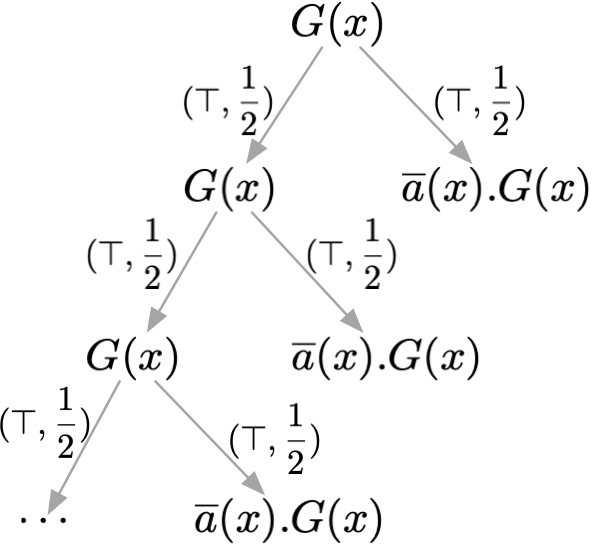
\includegraphics[width=5cm]{../figures/example1.png}
            \caption[]{$G(x)$的静态迁移树} 
            \label{fig_eg4_1}
         \end{figure}
         \begin{figure}[!htbp]
            \small
            \centering
            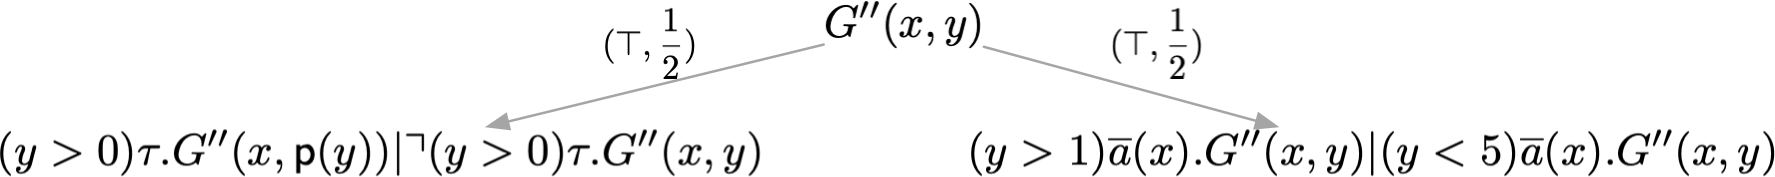
\includegraphics[width=13cm]{../figures/example4_2.png}
            \caption[]{$G''(x,y)$的静态迁移树} 
            \label{fig_eg4_2}
         \end{figure}

         对于$G(x)\rightsquigarrow_{\top\mathcal{S}}\stackrel{\frac{1}{2}}{\rightarrow}_{\top} [\overline{a}(x).G(x)]_{\top\mathcal{S}}$,
         存在集合$$\{G''(x,y)\rightsquigarrow_{\top\mathcal{S}}\stackrel{\frac{1}{2}}{\rightarrow}_{\top}[(y>1)\overline{a}(x).G''(x,y)|(y<5)\overline{a}(x).G''(x,y)]_{\top\mathcal{S}}\}$$
         其中$\mathsf{Th}\vdash (\top\Rightarrow\top)$且$\frac{1}{2}=\frac{1}{2}$,$(\overline{a}(x).G(x),(y>1)\overline{a}(x).G''(x,y)|(y<5)\overline{a}(x).G''(x,y))\in\mathcal{S}$。

         对于$G''(x,y)\rightsquigarrow_{\top\mathcal{S}}\stackrel{\frac{1}{2}}{\rightarrow}_{\top}[(y>1)\overline{a}(x).G''(x,y)|(y<5)\overline{a}(x).G''(x,y)]_{\top\mathcal{S}}$,
         我们可以对称地用集合$\{G(x)\rightsquigarrow_{\top\mathcal{S}}\stackrel{\frac{1}{2}}{\rightarrow}_{\top} [\overline{a}(x).G(x)]_{\top\mathcal{S}}\}$模拟。

         对于$G''(x,y)\rightsquigarrow_{\top\mathcal{S}}\stackrel{\frac{1}{2}}{\rightarrow}_{\top}[(y>0)\tau.G''(x,\mathsf{p}(y))|\urcorner(y>0)\tau.G''(x,y)]_{\top\mathcal{S}}$,
         由于等价关系具有传递性,$G''(x,y) \in [(y>0)\tau.G''(x,\mathsf{p}(y))|\urcorner(y>0)\tau.G''(x,y)]_{\top\mathcal{S}} = [G''(x,y)]_{\top\mathcal{S}}$。
      }
   \end{itemize}
   因此我们可以得出校长的判断是正确的。
\end{proof}
例~\ref{eg:5}是一个简单的例子,给出了同一系统的两种不同实现,
这两种实现在外界观察者的视角中是效果相同的,
即具有\textit{观察等价性}。
符号互模拟给观察等价性提供了严格的刻画,为观察者的\textit{主观感觉}提供了\textit{客观依据}。

\section{随机传值进程模型的等价性}

如~\ref{ch:symbolic_bisimulation}节中所述,
符号互模拟描述了$\mathbb{RVPC}_{\mathsf{Th}}$的观察等价性,
因此我们可以通过符号互模拟定义随机传值进程模型的等价性。

我们首先证明符号互模拟关系是一个等价关系,
众所周知一个等价关系应具有自反性、对称性、传递性。
根据定义~\ref{def:rvpc_symbolic_bisimulation},
容易得到符号互模拟具有自反性和对称性,
我们接下来证明符号互模拟的传递性。
\begin{lemma}\label{lemma:transitivity}
   符号互模拟具有传递性。
\end{lemma} 
\begin{proof}
   证明符号互模拟的传递性等价于证明若$\mathcal{E}$是一个符号互模拟,且$A\mathcal{E}B, B \mathcal{E} C$,则$A \mathcal{E} C$。
   \begin{itemize}
      \item[(1)] {
         若$A\rightsquigarrow_{\varphi \mathcal{E}}\stackrel{\lambda}{\rightarrow}_{\varphi} \mathcal{C}\in \mathcal{T}_{RVPC}/\varphi\mathcal{E},\mathcal{C}\neq [A]_{\varphi\mathcal{E}}$,
         由于$A\mathcal{E}B$,
         根据定义存在$\varphi$的划分$\{\varphi_i\}_{i\in I}$
         和集合$S=\{B\rightsquigarrow_{\varphi_i\mathcal{E}}\stackrel{\lambda}{\rightarrow}_{\psi_i}[\mathcal{C}]_{\varphi_i\mathcal{E}}|\mathsf{Th}\vdash \varphi_i\Rightarrow\psi_i\}_{i\in I}$。
         对于$B$关于$\varphi_i\mathcal{E}$的条件等价树$t^B_{\varphi_i\mathcal{E}}$上的节点$L$,
         因为$\mathsf{Th}\vdash\varphi_i\Rightarrow \psi_i$,
         若$L\stackrel{\lambda}{\rightarrow}_{\psi_i}L'\in [\mathcal{C}]_{\varphi_i\mathcal{E}}$,
         则$L\stackrel{\lambda}{\rightarrow}_{\varphi_i}L'\in [\mathcal{C}]_{\varphi_i\mathcal{E}}$,
         因此存在集合$S'=\{B\rightsquigarrow_{\varphi_i\mathcal{E}}\stackrel{\lambda}{\rightarrow}_{\varphi_i}[\mathcal{C}]_{\varphi_i\mathcal{E}}\}_{i\in I}$,
         根据定义~\ref{def:rvpc_symbolic_bisimulation},
         $S'$也可以作为$A\rightsquigarrow_{\varphi \mathcal{E}}\stackrel{\lambda}{\rightarrow}_{\varphi} \mathcal{C}\in \mathcal{T}_{RVPC}/\varphi\mathcal{E},\mathcal{C}\neq [A]_{\varphi\mathcal{E}}$的模拟。
      
         由于$B\mathcal{E}C$,对于每一个$B\rightsquigarrow_{\varphi_i\mathcal{E}}\stackrel{\lambda}{\rightarrow}_{\varphi_i}[\mathcal{C}]_{\varphi_i\mathcal{E}}$,
         根据定义存在$\varphi_i$的划分$\{\varphi_{i,j}\}_{j\in J}$
         和集合$S_i=\{C\rightsquigarrow_{\varphi_{i,j}\mathcal{E}}\stackrel{\lambda}{\rightarrow}_{\psi_{i,j}}[\mathcal{C}]_{\varphi_{i,j}\mathcal{E}}|\mathsf{Th}\vdash \varphi_{i,j}\Rightarrow \psi_{i,j}\}_{j\in J}$,
         和集合$S_i=\{C\rightsquigarrow_{\varphi_{i,j}\mathcal{E}}\stackrel{\lambda}{\rightarrow}_{\varphi_{i,j}}[\mathcal{C}]_{\varphi_{i,j}\mathcal{E}}\}_{j\in J}$。

         进而,存在$\varphi$的划分$Con=\bigcup_{i\in I}\{\varphi_{i,j}\}_{j\in J}$
         和集合$S'=\bigcup_{i\in I}S_i'$,使得$C$可以符号模拟$A$。
         对称的证明是完全一致的。
      }
      \item[(2)] {
         若$A\rightsquigarrow_{\varphi \mathcal{E}}\stackrel{q}{\rightarrow}_{\varphi} \mathcal{C}\in \mathcal{T}_{RVPC}/\varphi\mathcal{E},\mathcal{C}\neq [A]_{\varphi\mathcal{E}},q\in(0,1]$,
         由于$A\mathcal{E}B$,存在$\varphi$的划分$\{\varphi_i\}_{i\in I}$和集合$\{B\rightsquigarrow_{\varphi_i\mathcal{E}}\stackrel{q_i}{\rightarrow}_{\psi_i} [\mathcal{C}]_{\varphi_i\mathcal{E}}|\mathsf{Th}\vdash \varphi_i\Rightarrow \psi_i\wedge q=q_i\}$,
         因此存在$\{B\rightsquigarrow_{\varphi_i\mathcal{E}}\stackrel{q_i}{\rightarrow}_{\varphi_i} [\mathcal{C}]_{\varphi_i\mathcal{E}}\}$可以模拟$A$的条件$q$-迁移,
         余下部分与$l$-迁移的证明相同。
      }
   \end{itemize}
\end{proof}
证明了符号互模拟的传递性后我们可以得到定理~\ref{th:equality}。
\begin{theorem}\label{th:equality}
   符号互模拟关系是等价关系。
\end{theorem}

接下来我们希望通过符号互模拟定义$\mathbb{RVPC}_{\mathsf{Th}}$的观察等价性,
一种比较直接的想法是将$\mathbb{RVPC}_{\mathsf{Th}}$的符号互模拟的全集定义为
$\mathbb{RVPC}_{\mathsf{Th}}$的观察等价性,我们首先需要证明符号互模拟关系的全集仍然是符号互模拟关系。

\begin{lemma}\label{lemma:closure}
   如果每一个$\mathcal{T}_{\mathbb{RVPC}_{\mathsf{Th}}}$上的关系$\mathcal{E}_i$都是符号互模拟关系,
   那么$(\bigcup_{i\in I}\mathcal{E}_i)^*$是符号互模拟关系。
\end{lemma}
\begin{proof}
   令$\mathcal{E}=(\bigcup_{i\in I}\mathcal{E}_i)^*$。
   给定$A_0\mathcal{E}_{i_1}A_1\mathcal{E}_{i_2}A_2\dots A_{k-1}\mathcal{E}_{i_k} A_k$,
   由于$\mathcal{E}=(\bigcup_{i\in I}\mathcal{E}_{i})^*$,
   我们可以得到$A_1\mathcal{E}A_k$,
   若$\mathcal{E}$是一个符号互模拟关系,
   则对于条件$l$-迁移:$A_0\rightsquigarrow_{\varphi\mathcal{E}}\stackrel{\lambda}{\rightarrow}_{\varphi} \mathcal{C}\in \mathcal{T}_{\mathbb{RVPC}_{\mathsf{Th}}},\mathcal{C}\neq [A_0]_{\varphi\mathcal{E}}$,
   存在$\varphi$的划分$\{\varphi_i\}_{i\in I}$和集合
   $\{A_k\rightsquigarrow_{\varphi_i\mathcal{E}}\stackrel{\lambda}{\rightarrow}_{\psi_i}[\mathcal{C}]_{\varphi_i\mathcal{E}}|\mathsf{Th}\vdash \varphi_i\Rightarrow\psi_i\}$可模拟该操作。
   我们可以通过归纳的证明$A_0\mathcal{E}A_1$,$A_1$可以模拟$A_0$;
   $A_1\mathcal{E}A_2$,$A_2$可以模拟$A_1$;\dots;最终证明$A_k$可以模拟$A_0$。

   对于$A_0\rightsquigarrow_{\varphi\mathcal{E}}\stackrel{\lambda}{\rightarrow}_{\varphi} \mathcal{C}\in \mathcal{T}_{\mathbb{RVPC}_{\mathsf{Th}}},\mathcal{C}\neq [A_0]_{\varphi\mathcal{E}}$,
   我们需要给出$\varphi$的划分$\{\varphi_i\}_{i\in I}$
   和集合$\{A_1\rightsquigarrow_{\varphi_i\mathcal{E}}\stackrel{\lambda}{\rightarrow}_{\psi_i}[\mathcal{C}]_{\varphi_i\mathcal{E}}\}$
   来模拟$A_0$的动作。

   考虑$A_0\rightsquigarrow_{\varphi\mathcal{E}}\stackrel{\lambda}{\rightarrow}_{\varphi} \mathcal{C}\in \mathcal{T}_{\mathbb{RVPC}_{\mathsf{Th}}},\mathcal{C}\neq [A_0]_{\varphi\mathcal{E}}$,
   由等价集的定义,我们可以得出$\varphi\mathcal{E}$上的等价集$\mathcal{C}$可以被划分成不相交的$\varphi\mathcal{E}_{i_1}$上的等价集
   $\{\mathcal{C}_j^{i_1}\}$。
   假设$t_{A_0}$是$A_0$关于$\varphi\mathcal{E}$的条件等价树,
   我们可以递归的构建出$A_1$关于$\varphi\mathcal{E}$的条件等价森林。

   \begin{itemize}
      \item[(1)] {
         \textbf{$t_{A_0}$的根节点$A_0$只有一个儿子节点$A_0'$。}
         若$A_0'\in[A_0]_{\varphi\mathcal{E}_{i_1}}$,
         我们将以$\varphi A_0'$作为下次递归的根节点,
         构建$\varphi A_1$条件等价森林
         (这样递归是因为在$A_1$的$\varphi\mathcal{E}$条件等价森林中的所有节点的动作都满足条件$\varphi$,
         $A_1$和$\varphi A_1$是等价的)。
         若$A_0'\notin[A_0]_{\varphi\mathcal{E}_{i_1}}$,
         根据$A_0\mathcal{E}_{i_1}A_1$,
         我们可以得到$\varphi$的划分$\{\varphi_i\}_{i\in I}$
         和集合$\{A_1\rightsquigarrow_{\varphi_i\mathcal{E}_{i_1}}\stackrel{\tau}{\rightarrow}_{\psi_i}[\mathcal{C}]_{\varphi_i\mathcal{E}_{i_1}}|\mathsf{Th}\vdash \varphi_i\Rightarrow \psi_i\}_{i\in I}$。
         
         根据推论~\ref{lemma:transitivity}的证明经验,我们其实可以用$\{A_1\rightsquigarrow_{\varphi_i\mathcal{E}_{i_1}}\stackrel{\tau}{\rightarrow}_{\varphi_i}[\mathcal{C}]_{\varphi_i\mathcal{E}_{i_1}}\}_{i\in I}$
         模拟$A_0\rightsquigarrow_{\varphi\mathcal{E}}\stackrel{\tau}{\rightarrow}_{\varphi} \mathcal{C}\in \mathcal{T}_{\mathbb{RVPC}_{\mathsf{Th}}},\mathcal{C}\neq [A_0]_{\varphi\mathcal{E}}\}_{i\in I}$,
         为了方便证明,后续的证明中我们将直接使用$\{A_1\rightsquigarrow_{\varphi_i\mathcal{E}_{i_1}}\stackrel{\lambda}{\rightarrow}_{\varphi_i}[\mathcal{C}]_{\varphi_i\mathcal{E}_{i_1}}\}_{i\in I}$的形式。
         
         $\{A_1\rightsquigarrow_{\varphi_i\mathcal{E}_{i_1}}\stackrel{\tau}{\rightarrow}_{\varphi_i}[\mathcal{C}]_{\varphi_i\mathcal{E}_{i_1}}\}_{i\in I}$
         实际构建出了一个条件等价树的集合$\{t_{A_1}^{i}\}_{i\in I}$,
         对于每个条件等价树$t_{A_1}^i$的叶子节点$B$,$B\stackrel{\tau}{\rightarrow}_{\varphi_i}B'\in [A_0']_{\varphi_i\mathcal{E}_{i_1}}$,
         我们根据$\varphi_i A_0'$构建每一个$\varphi_i B'$关于$\varphi_i\mathcal{E}$的等价森林。
         此时将$B$所在的$\varphi_i\mathcal{E}$等价树$t_{A_1}^{i}$复制并
         与每个$B'$的$\varphi_i\mathcal{E}$的等价森林中的等价树相连,
         我们可以得到$A_1$关于$\varphi\mathcal{E}$的条件等价森林。
      }
      \item[(2)] {
         \textbf{$t_{A_0}$的根节点$A_0$有$h$个儿子节点$A_0^1,\dots,A_0^h$。}
         根据定义$A_0\stackrel{\coprod_{i\in [h]p_j\tau}}{\rightarrow}_{\psi} \coprod_{j\in [h]}A_0^j$,
         $A_0$到$A_0^j$的边被标记为$(\psi, p_j)$,其中$\varphi\Rightarrow\psi$。

         若所有$A_0^j\in [A_0]_{\varphi\mathcal{E}_{i_1}}$,
         我们将根据$\varphi A_0^1$构建$\varphi A_1$的条件等价森林。

         若存在$A_0^j\notin [A_0]_{\varphi\mathcal{E}_{i_1}}$,
         不妨设为$A_0^1$,则$A_0\rightsquigarrow_{\varphi\mathcal{E}_{i_1}}\stackrel{q}{\rightarrow}_{\varphi} [A_0^1]_{\varphi\mathcal{E}_{i_1}}$,
         根据$A_0\mathcal{E}_{i_1}A_1$,
         我们可以得到$\varphi$的划分$\{\varphi_i\}_{i\in I}$和集合
         $\{A_1\rightsquigarrow_{\varphi_i\mathcal{E}_{i_1}}\stackrel{q}{\rightarrow}_{\varphi_i} [A_0^1]_{\varphi_i\mathcal{E}_{i_1}}\}_{i\in I}$,
         这其中关系到$A_1$关于$\varphi_i\mathcal{E}_{i_1}$的条件等价树$t_1^i$,
         根据条件$q$-迁移的定义,
         存在$\mathsf{P}_{\varphi_i,\varphi_i\mathcal{E}_{i_1}}(N\stackrel{\coprod_{i'\in [h']}p_{i'}\tau}{\longrightarrow}_{\varphi_i} N'\in [A_0^1]_{\varphi_i\mathcal{E}_{i_1}}) = q$,
         我们根据$\varphi_i A_0^1$构建每个$\varphi_i N'$关于$\varphi_i\mathcal{E}$的条件等价森林。
      }
      \item[(3)] {
         \textbf{$t_{A_0}$的根节点$A_0$可以作$A_0\stackrel{\lambda}{\rightarrow}_{\varphi} L'$。}
         根据定义存在$\varphi$的划分$\{\varphi_i\}_{i\in I}$和集合
         $\{A_1\rightsquigarrow_{\varphi_i\mathcal{E}_{i_1}}\stackrel{\lambda}{\rightarrow}_{\varphi_i} [L']_{\varphi_i\mathcal{E}_{i_1}}\}$。
      }
   \end{itemize}

   上述递归的构建可以通过图~\ref{fig:equal_forest}更加形象的表述。
   \begin{figure}[!htbp]
      \small
      \centering
      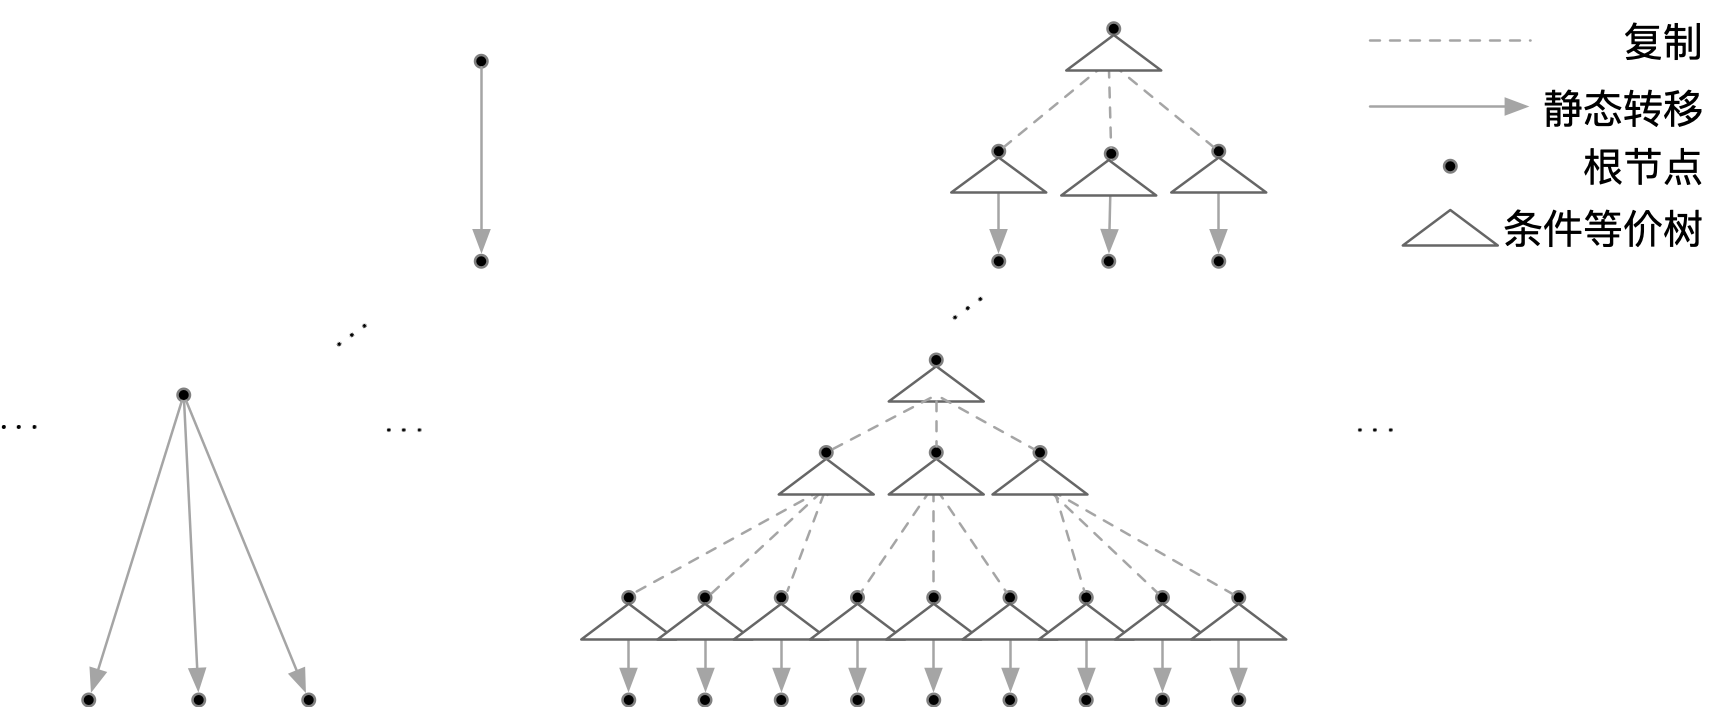
\includegraphics[width=13cm]{../figures/equality_1.png}
      \caption[]{递归构建图解} 
      \label{fig:equal_forest}
   \end{figure}
   图~\ref{fig:equal_forest}中,
   第一层描述了根节点只有一个儿子节点情况的构建方法,
   对于每一个$i\in I$,
   右侧的条件等价树都会复制一份,
   全部的条件等价树构成$\varphi\mathcal{E}$条件等价森林,
   作$\{A_1\rightsquigarrow_{\varphi_i\mathcal{E}_{i_1}\stackrel{\tau}{\rightarrow}_{\varphi_i}}[A_0']_{\varphi_i\mathcal{E}_{i_1}}\}$
   对$A_0\stackrel{\tau}{\rightarrow}_{\varphi\mathcal{E}_{i_1}}A_0'$的模拟。

   第二层描述了根节点有多个儿子节点情况的构建方法,
   对于每一个$A_0\rightsquigarrow_{\varphi\mathcal{E}_{i_1}}\stackrel{q}{\rightarrow}_{\varphi}$,
   右侧的条件等价树会复制一份,
   在对每一个$A_0\rightsquigarrow_{\varphi\mathcal{E}_{i_1}}\stackrel{q}{\rightarrow}_{\varphi} [A_0^1]_{\varphi\mathcal{E}_{i_1}}$
   模拟时,对模拟该动作的集合$\{A_1\rightsquigarrow_{\varphi_i\mathcal{E}_{i_1}}\stackrel{q}{\rightarrow}_{\varphi_i} [A_0^1]_{\varphi_i\mathcal{E}_{i_1}}\}_{i\in I}$
   中的每一个元素都复制一份条件等价树,再进行对应的模拟。

   通过上述构建方式,我们最终会构建出$A_1$关于$\varphi\mathcal{E}$的条件等价树或条件等价森林,
   来模拟$A_0\rightsquigarrow_{\varphi\mathcal{E}}\stackrel{\lambda}{\rightarrow}_{\varphi} \mathcal{C}\in \mathcal{T}_{\mathbb{RVPC}_{\mathsf{Th}}},\mathcal{C}\neq [A_0]_{\varphi\mathcal{E}}$。
   归纳地,我们可以构建出$A_2$对$A_1$关于$\varphi\mathcal{E}$的条件等价树或条件等价森林中的每一个条件等价树的迁移
   的条件等价森林……最终构建出$A_k$模拟$A_0\rightsquigarrow_{\varphi\mathcal{E}}\stackrel{\lambda}{\rightarrow}_{\varphi} \mathcal{C}\in \mathcal{T}_{\mathbb{RVPC}_{\mathsf{Th}}},\mathcal{C}\neq [A_0]_{\varphi\mathcal{E}}$的条件等价森林。

   对于条件$q$-迁移:$A_0\rightsquigarrow_{\varphi\mathcal{E}}\stackrel{q}{\rightarrow}_{\varphi}\mathcal{C}$的证明方法是相同的。
\end{proof}

我们希望定义符号互模拟关系的全集为$\mathbb{RVPC}_{\mathsf{Th}}$上的观察等价性,
但这样定义仍会存在问题:考虑$A\in\mathcal{T}_{\mathbb{RVPC}_{\mathsf{Th}}}$,
若$A$在$\varphi\mathcal{E}$下的条件等价树是无限延伸的,即没有叶子节点,
例如:
\begin{align*}
   % \begin{split}
   &A(x) \stackrel{def}{=} (\overline{a}(x).0|B(\epsilon)|C)\backslash \{a,b,c\} &\\
   &B\stackrel{def}{=}a(x).B(x)
   &B(x)\stackrel{def}{=} \frac{1}{2}\tau.\overline{b}(x).B\oplus \frac{1}{2}\tau.\overline{c}(x).B\\
   &C\stackrel{def}{=} b(x).C(x)
   &D\stackrel{def}{=} c(x).D(x)\\
   &C(x)\stackrel{def}{=} \overline{a}(x).C
   &D(x)\stackrel{def}{=} \overline{a}(x).D
   % \end{split}
\end{align*}
若定义等价关系$[A(x)]_{\mathcal{E}}=[B(x)|C|D]_{\mathcal{E}}=[B|C(x)|D]_{\mathcal{E}}=[B|C|D(x)]_{\mathcal{E}}$,
这时$A(x)$的$\top \mathcal{E}$条件等价树如图~\ref{fig:divergent}。
\begin{figure}[!htbp]
   \small
   \centering
   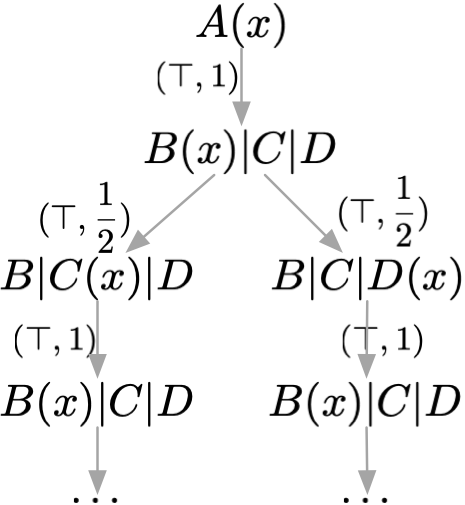
\includegraphics[width=3cm]{../figures/codivergent.png}
   \caption[]{$A(x)$的$\top \mathcal{E}$条件等价树} 
   \label{fig:divergent}
\end{figure}
在观察等价性的角度,我们认为$E(x)\stackrel{def}{=}\tau.E(x)$与$A(x)$应该是观察互模拟的,
然而,这时找到$A(x)$的条件$l$转移和条件$q$转移就会变得困难,
因此我们引入Uniform Approach中的共发散(codivergent)\cite{Fu_UniformApproach}的相关概念,并将其扩展为$\mathcal{T}){\mathbb{RVPC}_{\mathsf{Th}}}$下的共发散来解决这个问题。

\begin{definition}[发散]\label{def:divergent}
   对于$A\in\mathcal{T}_{\mathbb{RVPC}_{\mathsf{Th}}}$,
   若$A$在$\varphi\mathcal{E}$下的条件等价树为$t$,
   定义树$t$的分支$\pi$是$t$从根节点开始到叶节点结束的一条路径,
   定义$\pi(i)$为分支$\pi$上第$i$条边的标记中的概率部分,$\pi(i)\in(0,1]$。

   定义这条分支的概率$\mathsf{P}(\pi)=\prod\{\pi(i)|i\in [|\pi|]\}$,
   若这条分支是无穷的,则$\mathsf{P}(\pi)=\lim_{j\rightarrow \infty}\prod_{i=0}^{j}\pi(i)$。

   定义条件等价树的概率$\mathsf{P}(t)=\sum\{\mathsf{P}(\pi)|\pi\textrm{是}t\textrm{的一条分支}\}$。
   
   定义$t$的前$k$层分支的概率为$\mathsf{P}^k(t)=\sum \{\mathsf{P}(\pi)|\pi\textrm{是}t\textrm{的一条分支且}|\pi|\leq k\}$。

   定义$t$的有限长分支的概率$\mathsf{P}^f(t)=\lim_{k\rightarrow\infty}\mathsf{P}^k(t)$。

   当条件等价树$t$的有限长分支的概率$\mathsf{P}^f(t)=0$时,
   $t$称为\textit{发散的条件等价树},我们可以理解为$t$没有有限长的分支。
\end{definition}

通过定义~\ref{def:divergent},我们定义了使用符号互模拟关系的全集作为观察等价性时,
存在问题的情况,我们使用共发散的概念对这种情况的条件等价树的观察等价性单独定义。

\begin{definition}[共发散]
   若$\mathcal{E}$是$\mathcal{T}_{\mathbb{RVPC}_{\mathsf{Th}}}$上的等价关系,
   $\mathcal{E}$是一个共发散的等价关系当且仅当:
   当对于布尔表达式$\varphi$,
   条件等价集$\mathcal{C}\in\mathcal{T}_{\mathbb{RVPC}_{\mathsf{Th}}}/\varphi\mathcal{E}$,
   $\mathcal{C}$中的每一个元素关于$\varphi\mathcal{E}$的条件等价森林中的每一个棵树都是发散的条件等价树;
   或$\mathcal{C}$中的每一个元素关于$\varphi\mathcal{E}$的条件等价森林中的每一个棵树都不是发散的条件等价树。
\end{definition}

\begin{definition}
   $\mathcal{T}_{\mathbb{RVPC}_{\mathsf{Th}}}$上的观察等价性$=_{\mathbb{RVPC}_{\mathsf{Th}}}$定义为$\mathcal{T}_{\mathbb{RVPC}_{\mathsf{Th}}}$上的共发散的符号互模拟关系的全集。
\end{definition}
由于$=_{\mathbb{RVPC}_{\mathsf{Th}}}$仍然是一个符号互模拟关系,因此我们可以得到定理~\ref{th:equality2}。
\begin{theorem}\label{th:equality2}
   $=_{\mathbb{RVPC}_{\mathsf{Th}}}$是一个等价关系。
\end{theorem}

在数学特别是抽象代数中,同余关系或简称同余是相容于某个代数运算的等价关系。
设$A=<S,*,\delta>$是一个代数系统,$\sim$是载体$S$上的等价关系,若$\sim$在$A$上的所有运算下都是可保持的,则称$\sim$为代数系统$A$上的同余关系\cite{Cougruence}。 
同余关系使得元素所在的等价类在运算上可以作为一个整体来看待。
我们希望证明我们定义的$=_{\mathbb{RVPC}_{\mathsf{Th}}}$是一个同余关系。

\begin{theorem}
   $=_{\mathbb{RVPC}_{\mathsf{Th}}}$具有同余性。
\end{theorem}
\begin{proof}
   $=_{\mathbb{RVPC}_{\mathsf{Th}}}$对于随机选择和非确定性选择的可保持性比较容易证明。
   由推论~\ref{co:condition}易知$A=_{\mathbb{RVPC}_{\mathsf{Th}}}B$则$\varphi A=_{\mathbb{RVPC}_{\mathsf{Th}}}\varphi B$。
   为方便证明,以下$=_{\mathbb{RVPC}_{\mathsf{Th}}}$简记为$=$,绝对等价性记为$\equiv$,定义记为$\stackrel{def}{=}$。
   
   对于本地化操作子(Localization),对于$A=B,(a)A\rightsquigarrow_{\varphi=}\stackrel{\lambda}{\rightarrow}_{\varphi} (a)A'\notin [(a)A]_{\varphi =}, a\notin \lambda$,
   易知有$\varphi$的划分$\{\varphi_i\}_{i\in I}$和集合$\{(a)B\rightsquigarrow_{\varphi_i=}\stackrel{\lambda}{\rightarrow}_{\varphi_i}[(a)A]_{\varphi =}\}$。

   对于并发操作子(Composition),考虑等价关系$\mathcal{R}\stackrel{def}{=}\{(A|C,B|D)|(A,B)\in =,(C,D)\in =\}$,
   令$\mathcal{R}' = (\mathcal{R}\cup =)^*$,我们证明$\mathcal{R}'$是一个符号互模拟关系。
   对于条件$l$-迁移:$(A|C)\rightsquigarrow_{\varphi\mathcal{R'}}\stackrel{\lambda}{\rightarrow}_{\varphi}\mathcal{C}\in\mathcal{T}_{\mathbb{RVPC}_{\mathsf{Th}}}/\varphi \mathcal{R}',\mathcal{C}\neq [(A|C)]_{\varphi\mathcal{R}'}$,
   我们可以用引理~\ref{lemma:closure}中的方法递归的构造$(B|C)$的$\varphi\mathcal{E}$条件等价森林来模拟$(A|C)$的动作,
   令$t_{(A|C)}$为$(A|C)$关于$\varphi\mathcal{R'}$的条件等价树。
   \begin{itemize}
      \item[(1)] {
         $t_{(A|C)}$上的边:
         $A|C\stackrel{(\psi, 1)}{\rightarrow} A'|C, \mathsf{Th}\vdash \varphi\Rightarrow\psi$
         是由于$A\stackrel{\tau}{\rightarrow}_{\varphi} A'$。

         若$A'\in [A]_{\varphi =}$,
         那么$(A'|C)\in[(A|C)]_{\varphi\mathcal{R}'}\equiv[(B|D)]_{\varphi\mathcal{R}'}$。
         实际上,对于$A\stackrel{\coprod_{i\in I}p_i\tau}{\rightarrow}_{\varphi} \coprod_{i\in I} A_i=A$,
         $A_i|C\in [B|D]_{\varphi\mathcal{R}'}$。
         我们可以根据$\varphi (A_0|C)$的$\varphi\mathcal{R}'$条件等价树构建$(B|D)$的$\varphi\mathcal{R}'$条件等价森林。

         若$A'\notin [A]_{\varphi =}$,
         那么根据定义存在$\{B\rightsquigarrow_{\varphi_i\mathcal{=}}\stackrel{\tau}{\rightarrow}_{\varphi_i}B_i\in [A']_{\varphi_i =}\}_{i\in I}$,
         模拟$A\rightsquigarrow_{\varphi =}\stackrel{\tau}{\rightarrow}_{\varphi} A'$,
         其中$\{\varphi_i\}_{i\in I}$是$\varphi$的划分。
         我们根据$\varphi_i A'$构建$\varphi_i B_i$的$\varphi_i \mathcal{R}'$条件等价森林。
      }
      \item[(2)] {
         $t_{(A|C)}$上的边:
         $A|C\stackrel{(\psi, 1)}{\rightarrow} A'|C', \mathsf{Th}\vdash \varphi\Rightarrow\psi$
         是由于$A\stackrel{\overline{a}(t)}{\longrightarrow}_{\psi'} A', C\stackrel{a(x)}{\longrightarrow}_{\psi''} C', \psi=\psi'\psi''$。

         根据$A=B,C=D$,
         $A\rightsquigarrow_{\varphi = }\stackrel{\overline{a}(t)}{\longrightarrow}_{\varphi}A'$
         可以由$\{B\rightsquigarrow_{\varphi_i =}\stackrel{\overline{a}(t)}{\longrightarrow}_{\varphi_i}B_i\in [A']_{\varphi_i=}\}_{i\in I}$模拟,
         其中$\{\varphi_i\}_{i\in I}$是$\varphi$的划分。
         $C\rightsquigarrow_{\varphi = }\stackrel{a(x)}{\longrightarrow}_{\varphi}C'$
         可以由$\{D\rightsquigarrow_{\varphi_j =}\stackrel{a(x)}{\longrightarrow}_{\varphi_j}D_j\in [C']_{\varphi_j=}\}_{j\in J}$模拟,
         其中$\{\varphi_j\}_{j\in J}$是$\varphi$的划分。

         对于所有的$i\in I, j\in J, \mathsf{Th}\vdash \varphi_i\varphi_j\not\Rightarrow \bot$,
         $(B_i\mid D_j)\in[A'\mid C']_{\varphi_i\varphi_j \mathcal{R'}}$,
         我们根据$\varphi_i\varphi_j(A'|C')$的$\varphi_i\varphi_j \mathcal{R}' $条件等价树构建$\varphi_i\varphi_j(B_i|D_j)$的$\varphi_i\varphi_j \mathcal{R}' $条件等价森林。
      }
      \item[(3)] {
         $t_{(A|C)}$上的边:
         $A|C\stackrel{(\psi, q)}{\rightarrow} A'|C, \mathsf{Th}\vdash \varphi\Rightarrow\psi, q\in(0,1)$,
         则存在$A\stackrel{\coprod_{i\in I}p_i\tau}{\longrightarrow}_{\varphi} \coprod_{i\in I} A_i$,
         对所有的$i\in I$,$A|C\stackrel{(\psi, p_i)}{\rightarrow} A_i|C, \mathsf{Th}\vdash \varphi\Rightarrow\psi$。

         若对所有的$i\in I, A_i\in[A]_{\varphi =}$,我们可以根据$(A_i|C)$关于$\varphi\mathcal{R}'$的条件等价树构建$(B|D)$的$\varphi\mathcal{R}'$条件等价森林。

         若存在$A_i\notin [A]_{\varphi =}$,不妨设为$A_0$,
         若有$A_1\notin[A]_{\varphi =}\wedge A_1\in [A_0]_{\varphi =}$,
         此时有$A\rightsquigarrow_{\varphi = }\stackrel{q_0}{\rightarrow}_{\varphi}[A_0]_{\varphi=}$,
         $A\rightsquigarrow_{\varphi = }\stackrel{q_1}{\rightarrow}_{\varphi}[A_0]_{\varphi=}$,
         $A|C\rightsquigarrow_{\varphi = }\stackrel{q_0+q_1}{\longrightarrow}_{\varphi}[A_1|C]_{\varphi=}$。

         根据$A=B$,存在$\varphi$的划分$\{\varphi_i\}_{i\in I}$和集合
         $\{B\rightsquigarrow_{\varphi_i=}\stackrel{q_0}{\rightarrow}_{\varphi_i}B_i\in [A_0]_{\varphi_i =}\}$
         模拟$A\rightsquigarrow_{\varphi = }\stackrel{q_0}{\rightarrow}_{\varphi}[A_0]_{\varphi=}$。
         存在$\varphi$的划分$\{\varphi_j\}_{j\in J}$和集合
         $\{B\rightsquigarrow_{\varphi_j=}\stackrel{q_1}{\rightarrow}_{\varphi_j}B_j\in [A_1]_{\varphi_j =}\}$
         模拟$A\rightsquigarrow_{\varphi = }\stackrel{q_1}{\rightarrow}_{\varphi}[A_1]_{\varphi=}$。
         对所有的$i\in I, j\in J, \mathsf{Th}\vdash \varphi_i\varphi_j\not\Rightarrow \bot$,
         我们有$(B|D)\rightsquigarrow_{\varphi_i\varphi_j=}\stackrel{q_0+q_1}{\longrightarrow}_{\varphi_i\varphi_j}(B'|D)\in[A_0|C]_{\varphi_i\varphi_j=}$,
         我们根据$\varphi_i\varphi_j (A_0|C)$的$\varphi_i\varphi_j \mathcal{R}' $条件等价树构建$\varphi_i\varphi_j(B'|D)$的$\varphi_i\varphi_j \mathcal{R}' $条件等价森林。
      }
      \item[(4)] {
         若$(A|C)\stackrel{\lambda}{\rightarrow}_{\varphi} (A'|C), \lambda\neq \tau$,
         则$A\stackrel{\lambda}{\rightarrow}_{\varphi} A'$,
         根据定义存在$\varphi$的划分$\{\varphi_i\}_{i\in I}$和集合
         $\{B|D\rightsquigarrow_{\varphi_i=}\stackrel{\lambda}{\rightarrow}_{\varphi_i} [(A'|C)]_{\varphi_i=}\}$。
      }
   \end{itemize}
   对于条件$q$-迁移:$(A|C)\rightsquigarrow_{\varphi=}\stackrel{q}{\rightarrow}_{\varphi}\mathcal{C}$的证明方法是相同的。

   在上述证明中,若$(A,B)\in =$,且$A$关于$\varphi =$的条件等价树是发散的,
   根据定义可知$B$对应的条件等价森林中的条件等价树也是发散的,
   我们可以根据同样的扩展方法证明共发散对上述操作子的封闭性。
\end{proof}

\section{本章小结}
本章我们介绍了一种经典的并发进程模型——传值进程算子(The Value-Passing Calculus)
和它的一种实现$\mathbb{VPC}_{\mathsf{Th}}$,
我们分析了$\mathbb{VPC}_{\mathsf{Th}}$对比其他传值进程模型的优势——不依赖神域,是一个封闭的模型,因此具有很强的表达能力。
考虑到$\mathbb{VPC}_{\mathsf{Th}}$的优势和表达能力,
我们在$\mathbb{VPC}_{\mathsf{Th}}$的基础上进行概率扩展获得随机传值进程模型。

首先,
我们使用Uniform Approach中的方法为$\mathbb{VPC}_{\mathsf{Th}}$添加随机选择操作子,
扩展成为随机传值进程模型$\mathbb{RVPC}_{\mathsf{Th}}$,
并给出了随机传值进程模型$\mathbb{RVPC}_{\mathsf{Th}}$的语法和迁移语义。

其次,
为了给出$\mathbb{RVPC}_{\mathsf{Th}}$观察等价性的定义,
我们介绍了分支互模拟,分析了Uniform Approach
得到分支互模拟的随机版本的关键是将非概率的状态保持的静态迁移扩展为了概率下的状态保持的静态迁移树。
同时,我们引入了Uniform Approach中的等价集、$\mathbb{VPC}_{\mathbb{Th}}$中的符号互模拟的概念,
由于$\mathbb{RVPC}_{\mathsf{Th}}$中涉及到条件操作子,
我们不能直接使用Uniform Approach中的扩展方法。
因此我们将等价集的概念扩展为条件等价集,
参考Uniform Approach中等价树的概念,
定义了
$\mathcal{T}_{\mathbb{RVPC}_{\mathsf{Th}}}$的条件等价树。
为了解决条件操作子的问题,我们还提出了条件等价森林的概念,
进而提出使用条件等价森林模拟条件等价树的思想,
并使用条件等价树的概念
给出了$\mathcal{T}_{\mathbb{RVPC}_{\mathsf{Th}}}$的符号互模拟关系的定义,
也就是符号互模拟的概率版本。
为了解决无限的条件等价树无法得到符号互模拟关系的问题,
我们根据Uniform Approach共发散的概念提出了$\mathbb{RVPC}_{\mathsf{Th}}$上共发散的定义,
我们将共发散的符号互模拟的全集定义为$\mathbb{RVPC}_{\mathsf{Th}}$的观察等价性,
并证明了$\mathbb{RVPC}_{\mathsf{Th}}$观察等价性是一个同余关系。
% !TeX root = ../thesis.tex

\chapter{随机传值进程模型的应用}\label{ch:gossip}

如前文所述,传值进程模型可以用于对通信协议的形式刻画,
我们可以使用随机传值进程模型对引入了随机性的通信协议进行形式刻画。
本章中我们使用随机传值进程模型对一种云计算协议
Gossip-Style Membership Protocol进行建模和模拟实现。

\section{Gossip-Style Membership协议}
\subsection{Gossip协议}
Gossip协议,也称为流言协议,传染病协议(Epidemic Protocol)是一个基于传染病传播方式的点对点通信协议。

Gossip协议可以被解释为办公室流言的传播:
每一个职员会随机和另一个职员分享最近的流言,
被分享者得知流言后会随机的和其他人分享,
在一次分享中,被分享者或许已经知道了这个流言。
比如有一天,小赵传出老板的一个谣言,
他在一次会议结束时将这个谣言告诉了小钱;
小钱得知了谣言后,又在一次会议后将它告诉了小李;
小李在一次会议后告诉小孙时,
发现小孙已经从小王那里知道了这个谣言。

Gossip protocol 最早是在1987年在Epidemic Algorithms for Replicated Database Maintenance中被提出。
主要用在分布式数据库系统中各个副本节点同步数据之用,这种场景的一个最大特点就是组成的网络的节点都是对等节点,是非结构化网络。
Bitcoin就是使用了Gossip协议来传播交易和区块信息。

Gossip协议中,节点之间的通信方式有三种:
\begin{itemize}
   \item {
      \textbf{Push Gossip:} 
      
      消息的发送者周期性的随机选择$k$个目标节点发送Gossip Message。
      接收到Gossip Message的节点可以根据本地时间,
      周期性的选择$k$个目标节点发送Gossip Message。
      在发送过程中,
      已经拥有Gossip Message的节点仍然可以被选为目标节点。
   }
   \item {
      \textbf{Pull Gossip:}

      每个节点周期性的向$k$个目标节点发送Gossip Query,
      收到Gossip Query的节点若拥有Gossip Message的节点会向发送Query的节点返回Gossip Message的拷贝。
   }
   \item {
      \textbf{Push/Pull Gossip:}

      在超过$\frac{n}{2}$的节点拥有Gossip Message时,可以证明此时选择Pull Gossip会比Push Gossip传播的更快[cite]。
      因此在使用Gossip协议时,常使用Push Gossip与Pull Gossip的混合:
      在消息传播$\frac{n}{2}$节点之前使用Push Gossip,在消息传播$\frac{n}{2}$之后使用Pull Gossip。
   }
\end{itemize}

\subsection{Membership协议}

Membership协议为集群中的每个节点提供了一个本地的列表,
成为Membership List,用来维护集群中其他节点的信息。
Membership协议提供了两个主要的服务:
\begin{itemize}
   \item 检测失效的节点
   \item 传播消息,如:告知其他节点失效信息
\end{itemize}

常见的Membership协议有
Heartbeating Protocol, 
Gossip-Style Membership Protocol, 
SWIM Failure Detector Protocol等。

\section{Gossip-Style Membership的实现}
我们使用$\mathbb{RVPC}_{\mathsf{Th}}$来实现Gossip-Style Membership协议,
来作为使用随机传值进程模型建模通信过程的示例,
类似的,也可以使用同样的建模方法建模其他现实问题。

由于Membership可以看作节点内部的功能,我们可以首先实现Gossip协议,将网络建立起来。

\subsection{Gossip协议的实现}\label{ch:gossip_impl}
由于Push Gossip的机制比较简单,
并且单一的Push Gossip协议仍然可以达到$O(\log N)$时间复杂度的消息传播,
本节我们使用$\mathbb{RVPC}_{\mathsf{Th}}$来建模以Push Gossip作为通信机制的Gossip协议。

我们首先来建模以Gossip协议为通信的Peer-to-Peer Sysyem的节点。
根据根据Gossip协议的定义,
我们可以从单一节点周期性的发送消息,
这意味着我们需要一个计时器机制,
我们选择在节点外部使用计时器周期性的通知节点发送消息,
节点的$\overline{time}$端口用于向计时器设置计时开始,
$timeout$端口用于接收计时器传来的timeout信号。
由于节点本身不产生和存储消息,
我们需要使用$accept$端口接收P2P系统外界消息,
使用$\overline{deliver}$向P2P系统外界传递节点在P2P系统中从其他节点收到的消息。
由于现实网络是复杂的,
我们将每一对节点之间的消息传播路径抽象为单独的、单工的通道,
如节点$Node_i$向$Node_j$传播消息时,
消息会在$trans_{i,j}$通道中,
从$Node_i$节点的$\overline{trans_{i,j}}$端口发出,
从$Node_j$节点的$trans_{i,j}$端口接收。
这里的消息传输方式实际上是信息的逻辑传输路径,
信息的物理传输路径可能是十分复杂且动态的,
我们可以将系统中节点的编号简单的理解为Socket通信中的IP地址:端口号,
每一个节点代表了某台主机上的某个进程。

Gossip单节点的通道示意图如图~\ref{fig:gossip_node_1}和
以Gossip协议作为通信协议的四节点的Peer-to-Peer Sysyem的示意图如图
~\ref{fig:p2p_system}。

\begin{figure}[!htp]
   \begin{minipage}{0.3\textwidth}
   \centering
   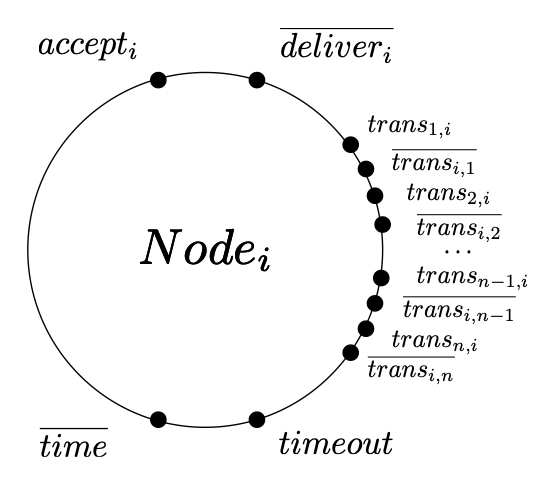
\includegraphics[width=5cm]{../figures/Node_gossip2.png}
   \caption{Gossip 节点示意图}
  \label{fig:gossip_node_1}
\end{minipage}\hfill
\begin{minipage}{0.6\textwidth}
   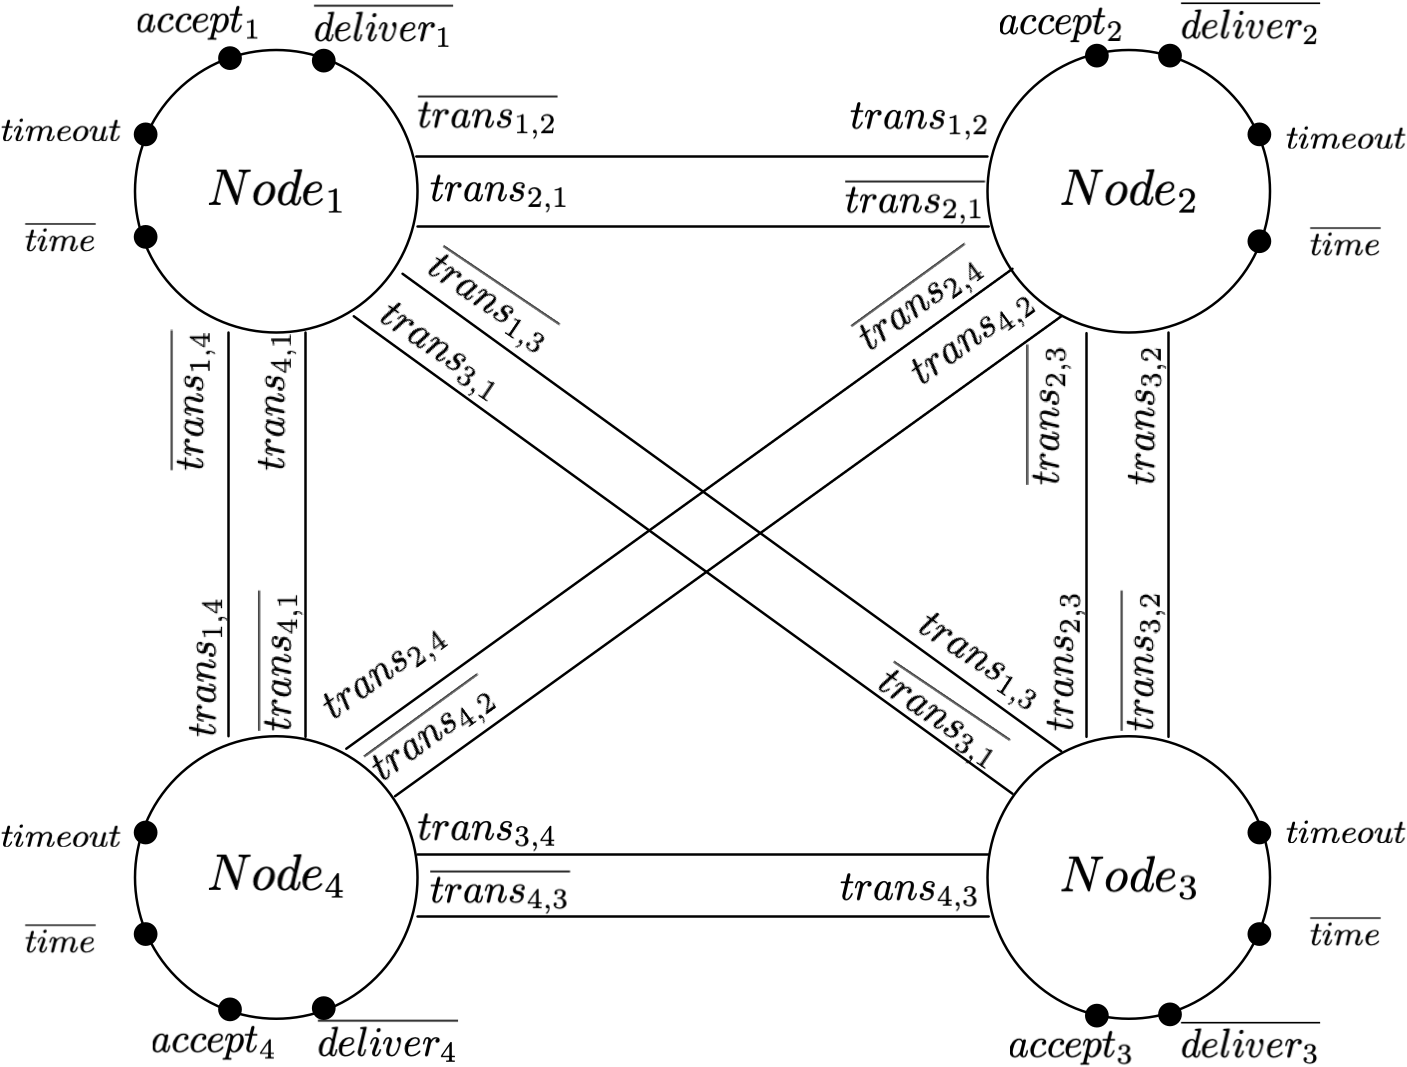
\includegraphics[width=8cm]{../figures/GossipSystem.png}
   \caption{基于Gossip协议的四节点P2P系统结构}
   \label{fig:p2p_system}
\end{minipage}
 \end{figure}

Gossip节点Node的状态有以下几种,分别对应Gossip协议中节点的状态:
\begin{table}[!hpt]
    \caption{节点状态对应}
    \label{tab:firstone}
    \centering
    \begin{tabular}{@{}llr@{}} \toprule
    %   \multicolumn{2}{c}{Item} \\ \cmidrule(r){1-2}
      节点状态 & Gossip状态 \\ \midrule
      Node&可接受系统外信息(除此状态其余状态均无法接收外界信息)\\
      DeliveringNode&可向系统外传递信息\\
      UnInfectiousNode&未获取Gossip Message\\
      InfectiousNode&已获取Gossip Message\\
      GossipingNode&可向系统内部特定b个其他节点发送Gossip Message\\ \bottomrule
    \end{tabular}
  \end{table}

基于以上定义的节点结构和节点状态,
我们定义一个基于Gossip协议的P2P系统。
\begin{align*}
   Node_i& \stackrel{def}{=} accept_i(x).DeliveringNode_i(x)\\
   DeliveringNode_i(x) &\stackrel{def}{=} \overline{deliver_i}(x).InfectiousNode_i(x)\\
   InfectiousNode_i(x)&\stackrel{def}{=}timeout.(\bigoplus_{perm\in \mathsf{PERM}_i} p_{perm}\tau.GossipingNode_{i,perm}(x))\\
%    &+\sum_{j\in \mathsf{N}/\{i\}}trans_{j,i}(x).DeliveringNode_i(x)\\
   GossipingNode_{i,perm}(x)&\stackrel{def}{=}\overline{trans_{i,perm_{1}}}(x).\dots \overline{trans_{i,perm_{b}}}(x).\overline{time}.InfectiousNode_i(x)\\
   UnInfectiousNode_i &\stackrel{def}{=} \sum_{j\in \mathsf{N}/\{i\}}trans_{j,i}(x).DeliveringNode_i(x)\\
   GossipSystem_\mathsf{N}&\stackrel{def}{=}(Node_1\mid UnInfectiousNode_2\mid \dots \mid UnInfectiousNode_n)\\
   &\backslash \{trans_{i,j}\mid i\in \mathsf{N} \wedge j\in \mathsf{N} \wedge i\neq j\}\cup \{time, timeout\}
\end{align*}
在这个P2P系统中共有$n$个节点,标号为$\mathsf{N}=\{1,2,\dots, n\}$,
每一个拥有Gossip Message的节点周期性的向$\mathsf{k}(\mathsf{k}\leq n-1)$
个其他节点发送Gossip Message。
其中$\mathsf{PERM}_i$为$\mathsf{N}/\{i\}$中任选$\mathsf{k}$个元素的全排列,
$p_{\mathsf{perm}}$为向一个特定的排列$perm$发送Gossip Message的概率,
为了方便建模,
我们假设一个节点选择任意其他节点作为Gossip的目标节点的概率是相同的,
即$p_{perm} = \frac{1}{A_{n-1}^{\mathsf{k}}} = \frac{(n-\mathsf{k}-1)!}{(n-1)!}$为固定值,
当$\mathsf{k}=2$时,$p_{perm} = \frac{1}{(n-1)(n-2)}$。

我们可以看到节点$Node_i$接受到外界消息$x$后,
迁移为$DeliveringNode_i(x)$的状态,
向外界递送这个消息,
进而迁移为$InfectiousNode)i(x)$的状态,
可以在接受到$timeout$信号时以概率$p_{\mathsf{perm}}$
的概率选定$\mathsf{N}/\{i\}$中任选$\mathsf{k}$个元素的全排列
中的一个排列$perm$作为发送目标,
进而迁移为$GossipingNode_{i,perm}(x)$,
向$perm$中的节点发送Gossip Message,
发送完成后回到$InfectiousNode_i(x)$的状态。
在一个$GossipSystem_{\mathsf{N}}$中,
还有状态为$InfectiousNode_i$的节点,
这些节点在接受了来自其他节点的Gossip Message时会迁移到$DeliveringNode_i(x)$的状态。
为了后面的分析,上述定义基于一系列理想条件的假设:
\begin{itemize}
   \item [(1)] {网络传输可靠。
   然而现实中的网络传输存在丢包、延迟、比特反转等问题,
   我们可以通过ACK机制来解决[cite]。
   对不可靠网络下的Gossip协议,我们可以在上述理想条件下增加对网络传输的过程的建模,建模过程在Milner的CCS中有提及
   [cite]。
   }
   \item [(2)] {节点不会损坏。
   在现实中节点(主机)在运行了一定时间后就会出现问题,
   对于多个节点构成的P2P系统,
   存在节点失效的概率只会更高[cite(MTTF)],
   Membership协议是用来探测节点失效的一种方式。
   }
   \item [(3)] {
      系统中只存在一个消息的传输。
      对于单个消息源的多个消息,我们仍然可以看作单个Gossip Message一起发送;
      对于多个消息源,我们可以为每个节点提供消息队列机制来保存多个消息,
      后文对Membership的建模提供了一个多消息源的解决思路。
      }
\end{itemize}

\subsection{Gossip协议的等价性}
% Brewer在CAP定理[cite]说到,
% 在分布式环境中设计和部署应用程序时,
% 存在特殊关系中的三个核心系统需求,
% 分别是一致性、可用性和分区容忍度。
% 其中一致性指一致性是指分布式系统中的多个服务节点,给定一系列的操作,在约定协议的保障下,使它们对外界呈现的状态是一致的。
% 分布式系统中的一致性按照对一致性要求的不同,主要分为严格一致性,强一致性,弱一致性和最终一致性这四大类。
% Gossip协议具有最终一致性。

Gossip协议的目的是为了在系统内对节点进行多播,
我们可以定义一个多播的规约,
证明~\ref{ch:gossip_impl}节中我们使用$\mathbb{RVPC}_{\mathsf{Th}}$实现的基于Gossip协议的P2P系统满足这个规约,
在进程演算中,我们需要证明二者互模拟。
由于我们在~\ref{ch:gossip_impl}节中实现的是单消息源单个消息的传播,
在多播的定义中同样我们只关注单消息源单个消息的多播。
\begin{definition} 单消息源的多播规约定义如下:
\begin{align*} 
    MulticastSpec_\mathsf{N}&\stackrel{def}{=}accept_1(x).\overline{deliver_1}(x).Multicasting_{\mathsf{N},\{1\}}(x)\\
    Multicasting_{\mathsf{N},\mathsf{KNOWN}}(x)&\stackrel{def}{=}\overline{deliver_i}(x).Multicasting_{\mathsf{N},\mathsf{KNOWN}\cup\{i\}}(x), \\
    &i\in \mathsf{N}-\mathsf{KNOWN} \wedge |\mathsf{N}|\neq |\mathsf{KNOWN}|
 \end{align*}
\end{definition} 
其中$|\mathsf{KNOWN}|$为已经得到此消息的节点编号集合,
节点可以通过$deliver$通道告知通信系统外(如本地的其他进程)节点已收到信息。
若一个节点对系统外通过$deliver$通道传递了这个消息,
我们将这个节点加入$|\mathsf{KNOWN}|$,
表示这个节点已经收到了消息。

 \begin{definition} 
   由于$GossipSystem_{\mathsf{N}}$中的节点可能处于:$InfectiousNode$,$DeliveringNode$,$UnInfectiousNode$
   三种状态(我们将$GossipingNode$的状态合并进了$InfectiousNode$),
   在后续的证明过程中表示起来比较冗长,
   为了方便后续的证明,我们给出特定状态下的
   $GossipSystem_{\mathsf{N}}$的记法,
   其中Composition算子符合交换律。
    \begin{align*}
   &GossipSystem_{\mathsf{N},(a,b,c)}(x)\\
   &= (\stackrel{a}{\overbrace{InfectiousNode(x)\mid \dots \mid InfectiousNode(x)}}\\
   &\mid \stackrel{b}{\overbrace{DeliveringNode(x)\mid \dots\mid DeliveringNode(x)}}\\
   &\mid \stackrel{c}{\overbrace{UnInfectiousNode\mid \dots \mid UnInfectiousNode}})\\
   &\backslash \{trans_{i,j}\mid i\in \mathsf{N} \wedge j\in \mathsf{N} \wedge i\neq j\}\cup \{time, timeout\}
\end{align*}
 \end{definition}
 其中,$GossipSystem_{\mathsf{N},(a,b,c)}(x)$表示
 在系统的$n=|\mathsf{N}|$个节点中,有$a$个处于$InfectiousNode(x)$的状态,
 有$b$个处于$DeliveringNode(x)$的状态,
 有$c$个处于$UnInfectiousNode$的状态,
 且满足$a+b+c=n$。
 很显然,初始的$GossipSystem_{\mathsf{N}}$中唯一的$Node$状态的节点此时已经从外界接收了某个消息$x$。

 接下来我们来证明,我们实现的基于Gossip协议的P2P系统满足多播系统的规约。
 由于$GossipSystem_{\mathsf{N}}$和$MulticastSpec_\mathsf{N}$中的每一个节点能且仅能执行一次$deliver$操作,
 且$deliver$的顺序不影响功能,
所以我们可以规定$A\stackrel{\overline{deliver_i}(t_1)}{\longrightarrow}_{\top} B$和$C\stackrel{\overline{deliver_j}(t_2)}{\longrightarrow}_{\top}B$是互模拟的当且仅当$t_1=t_2$,对下标是否一致不作要求。
因此在后文的证明中忽略了下标。
\begin{theorem}
    $GossipSystem_{\mathsf{N}} =_{\mathbb{RVPC}_{\mathsf{Th}}} MulticastSpec_{\mathsf{N}}$,$\mathsf{Th}$是可判定的逻辑。
\end{theorem}
\begin{proof}

我们可以通过构建等价集,并证明等价集是一个符号互模拟关系
来证明$GossipSystem_{\mathsf{N}} =_{\mathbb{RVPC}_{\mathsf{Th}}} MulticastSpec_{\mathsf{N}}$。

构造等价集
\begin{align*}
   \mathcal{S}&=\{(GossipSystem_{\mathsf{N}}, MulticastSpec_{\mathsf{N}}), \\
      &(GossipSystem_{\mathsf{N},(n,0,0)}(x), Multicasting_{\mathsf{N},\mathsf{N}}(x))\}\\
      & \cup \{(GossipSystem_{\mathsf{N},(a,b,c)}(x), Multicasting_{\mathsf{N}, \mathsf{KNOWN}}(x))\mid |\mathsf{KNOWN}| = a\neq n\}
\end{align*}

我们来依次证明$\mathcal{S}$中的每一对等价关系为符号互模拟关系:
\begin{itemize}
    \item {
       $GossipSystem_{\mathsf{N},(n,0,0)}(x)$和$Multicasting_{\mathsf{N},\mathsf{N}}(x)$的$\top \mathcal{S}$条件等价树分别只有一个根节点,
       且不能转移至其他等价集,他们的互模拟是显然的,实际上$GossipSystem_{\mathsf{N},(n,0,0)}(x)=Multicasting_{\mathsf{N},\mathsf{N}}(x)=0$。
    }
    \item {
        对于$(GossipSystem_{\mathsf{N},(a,b,c)}(x), Multicasting_{\mathsf{N}, \mathsf{KNOWN}}(x))\mid |\mathsf{KNOWN}| = a\neq n$:

        % 对应的$Multicasting_{\mathsf{N}, \mathsf{KNOWN}}(x)\rightsquigarrow_{\top\mathcal{S}}\stackrel{\overline{deliver}(x)}{\longrightarrow}_{\top\mathcal{S}} []$
        \begin{itemize}
            \item {\textbf{Case 1: $a<n-1$。}
            $GossipSystem_{\mathsf{N},(a,b,c)}(x)$的$\top \mathcal{S}$条件等价树 $t$如图~\ref{fig:epsilon_1}所示。
            \begin{figure}[!htbp]
            	\small
            	\centering
            	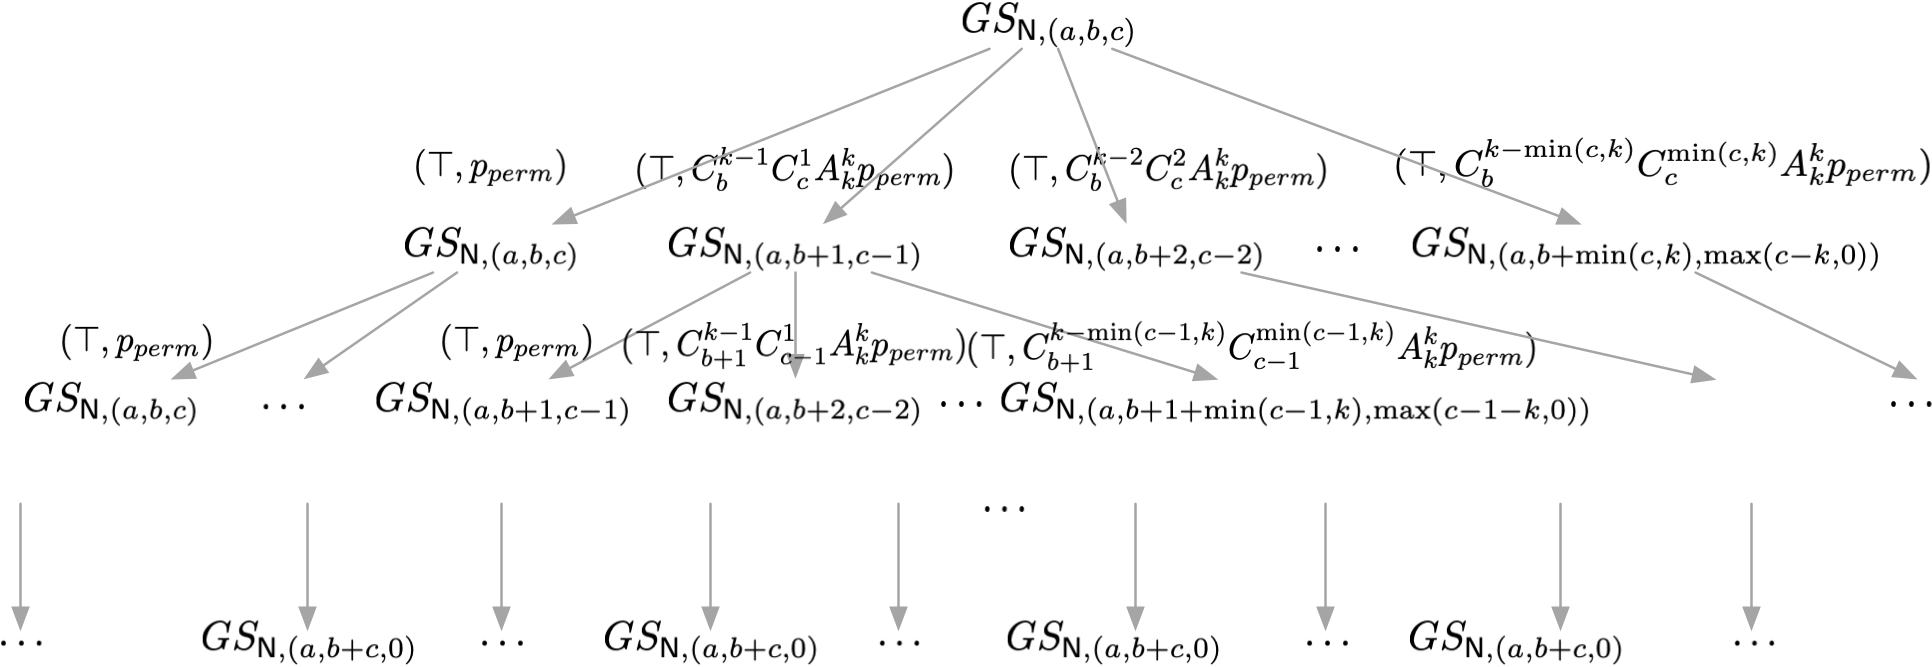
\includegraphics[width=14cm]{../figures/epsilon_tree1.png}
                \caption{\textbf{$GossipSystem_{\mathsf{N},(a,b,c)}(x)$关于$\top\mathcal{S}$的条件等价树 $t$}}
                \label{fig:epsilon_1}
            \end{figure}
            当$t$上的节点进入$GossipSystem_{\mathsf{N},(a,b+c,0)}(x)$状态时,
            状态保持的静态迁移($\tau$动作)就会终止,
            因此$GossipSystem_{\mathsf{N},(a,b+c,0)}(x)$为$t$的叶子结点。
            很显然,对$t$上的每一个非叶结点,都会经过$Node_j\stackrel{p'_j}{\rightarrow}_{\top}GossipSystem_{\mathsf{N},(a,b+c,0)}(x),p'_j=p_{j_1}p_{j_2}\dots p_{j_m}<1$。
            对$t$的叶子结点有$GossipSystem_{\mathsf{N},(a,b+c,0)}(x)\stackrel{\overline{deliver}(x)}{\longrightarrow}_{\top} GossipSystem_{\mathsf{N},(a+1,b+c-1,0)}(x)$。
            即
            $$GossipSystem_{\mathsf{N},(a,b,c)}(x)\rightsquigarrow_{\top\mathcal{S}}\stackrel{\overline{deliver}(x)}{\longrightarrow}_{\top}[GossipSystem_{\mathsf{N},(a+1,b',c')}(x)]_{\top\mathcal{S}}$$
            其中$b'+c'=b+c-1$。
            我们可以用$$Multicasting_{\mathsf{N},\mathsf{KNOWN}}\rightsquigarrow_{\top\mathcal{S}}\stackrel{\overline{deliver}(x)}{\longrightarrow}_{\top} Multicasting_{\mathsf{N}, \mathsf{KNOWN}'}$$来模拟上述状态迁移。
            对称的模拟依然成立。
            }
            \item {\textbf{Case 2: $a=n-1$。}
            \begin{itemize}
               \item {
                  {\textbf{Case 2.1:} $b=1$。}
                  $GossipSystem_{\mathsf{N},(n-1,1,0)}(x)$的$\top \mathcal{S}$条件等价树 $t$只有一个根节点,对于
                  $(GossipSystem_{\mathsf{N},(n-1,1,0)}(x)\rightsquigarrow_{\top\mathcal{S}}\stackrel{\overline{deliver}(x)}{\longrightarrow}_{\top}[GossipSystem_{\mathsf{N},(n,0,0)}(x)]_{\top\mathcal{S}}$,
                  我们可以用$Multicasting_{\mathsf{N},\mathsf{KNOWN}}\rightsquigarrow_{\top\mathcal{S}}\stackrel{\overline{deliver}(x)}{\longrightarrow}_{\top} Multicasting_{\mathsf{N}, \mathsf{N}}$来模拟。
               }
               \item {
                  {\textbf{Case 2.1:} $b=0$。}
                  $GossipSystem_{\mathsf{N},(n-1,0,1)}(x)$的$\top \mathcal{S}$条件等价树 $t$如图~\ref{fig:epsilon_2}所示。
                  \begin{figure}[!htbp]
                     \small
                     \centering
                     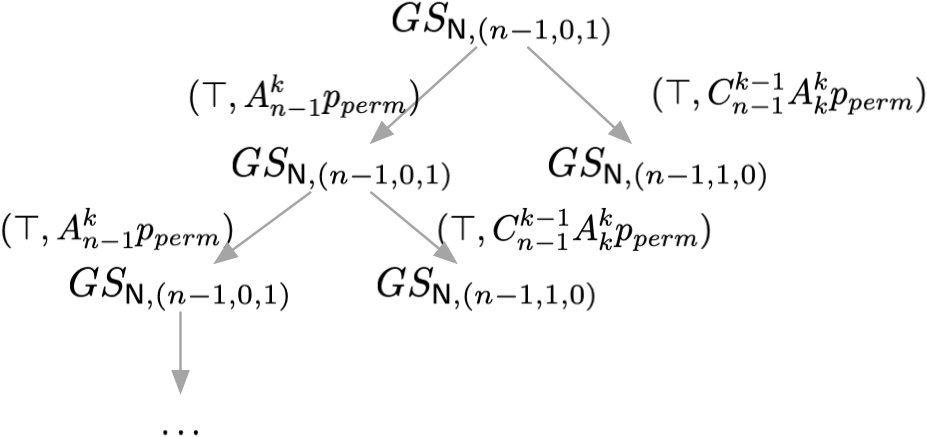
\includegraphics[width=8cm]{../figures/epsilon_tree_2.png}
                      \caption{\textbf{$GossipSystem_{\mathsf{N},(a,b,c)}(x)$关于$\top\mathcal{S}$的条件等价树 $t$}}
                      \label{fig:epsilon_2}
                  \end{figure}
                  
                  $GossipSystem_{\mathsf{N},(n-1,1,0)}$为$t$的叶节点,
                  且有$(GossipSystem_{\mathsf{N},(n-1,0,1)}(x)\rightsquigarrow_{\top\mathcal{S}}\stackrel{\overline{deliver}(x)}{\longrightarrow}_{\top}[GossipSystem_{\mathsf{N},(n,0,0)}(x)]_{\top\mathcal{S}}$。
                  我们可以用$Multicasting_{\mathsf{N},\mathsf{KNOWN}}\rightsquigarrow_{\top\mathcal{S}}\stackrel{\overline{deliver}(x)}{\longrightarrow}_{\top} Multicasting_{\mathsf{N}, \mathsf{N}}$来模拟。
               }
            \end{itemize}
            }
        \end{itemize}
    }
    \item {
        对$(GossipSystem_{\mathsf{N}}, MulticastSpec_{\mathsf{N}})$,
        我们可以用$$GossipSystem_{\mathsf{N}}\stackrel{accept(x).\overline{deliver(x)}}{\longrightarrow}_{\top}GossipSystem_{\mathsf{N},(1,0,0)}(x)$$
        $$MulticastSpec_{\mathsf{N}}\stackrel{accept(x).\overline{deliver(x)}}{\longrightarrow}_{\top}Multicasting_{\mathsf{N},\{1\}}$$来相互模拟。
    }
 \end{itemize}
\end{proof}
\subsection{Gossip-Style Membership的实现}

\subsubsection{Gossip Style Membership Protocol}
Renesse等人提出了一种基于Gossip协议的错误检测机制:
在集群中的每一个节点会维护一个列表Membership List,列表中包含已知的其他节点的\textit{地址}和整数表示的\textit{心跳}。
在每一个Gossip的周期,节点会增加自己的心跳,
并且随机的向另一个节点发送自己的Membership List;
若节点收到了其他节点发送过来的Membership List,
它会将两个列表合并,保留对应地址心跳最大的项。
若节点的Membership List的一项经过$T_{fail}$时间没有更新,则认为这一项对应的节点失效。

在本次的实现中,我们规定在每一个Gossip周期中,
节点可以随机选择$k$个节点发送自己的Membership List。

\subsubsection{对GossipSystem的调整}\label{ch:membership_system}
由于Gossip-Style Membership无需与外界的输入输出,并且需要提供储存、更新Membership List的函数,
我们需要对之前的节点结构进行调整。
同时,系统内的节点也会有失效的可能,我们可以用$p_{fail}$来定义一个节点失效的概率,
同时经过一个静态迁移$\tau$,这个节点就会被修复。
另外,由于在系统中的所有节点都是消息源,
且Membership List在系统中不停的更新,
因此也没有了感染者与被感染者的角色区分,
也需要对名称进行了修改。

在Gossip System节点的基础上,
将原本对外暴露的$accept,deliver$通道用于连接$Membership$,
作为链接网络的节点获取和更新本地Membership List的通道,
修改后的节点如图
\ref{fig:membership_node}
所示。

\begin{figure}[!htbp]
	\small
	\centering
	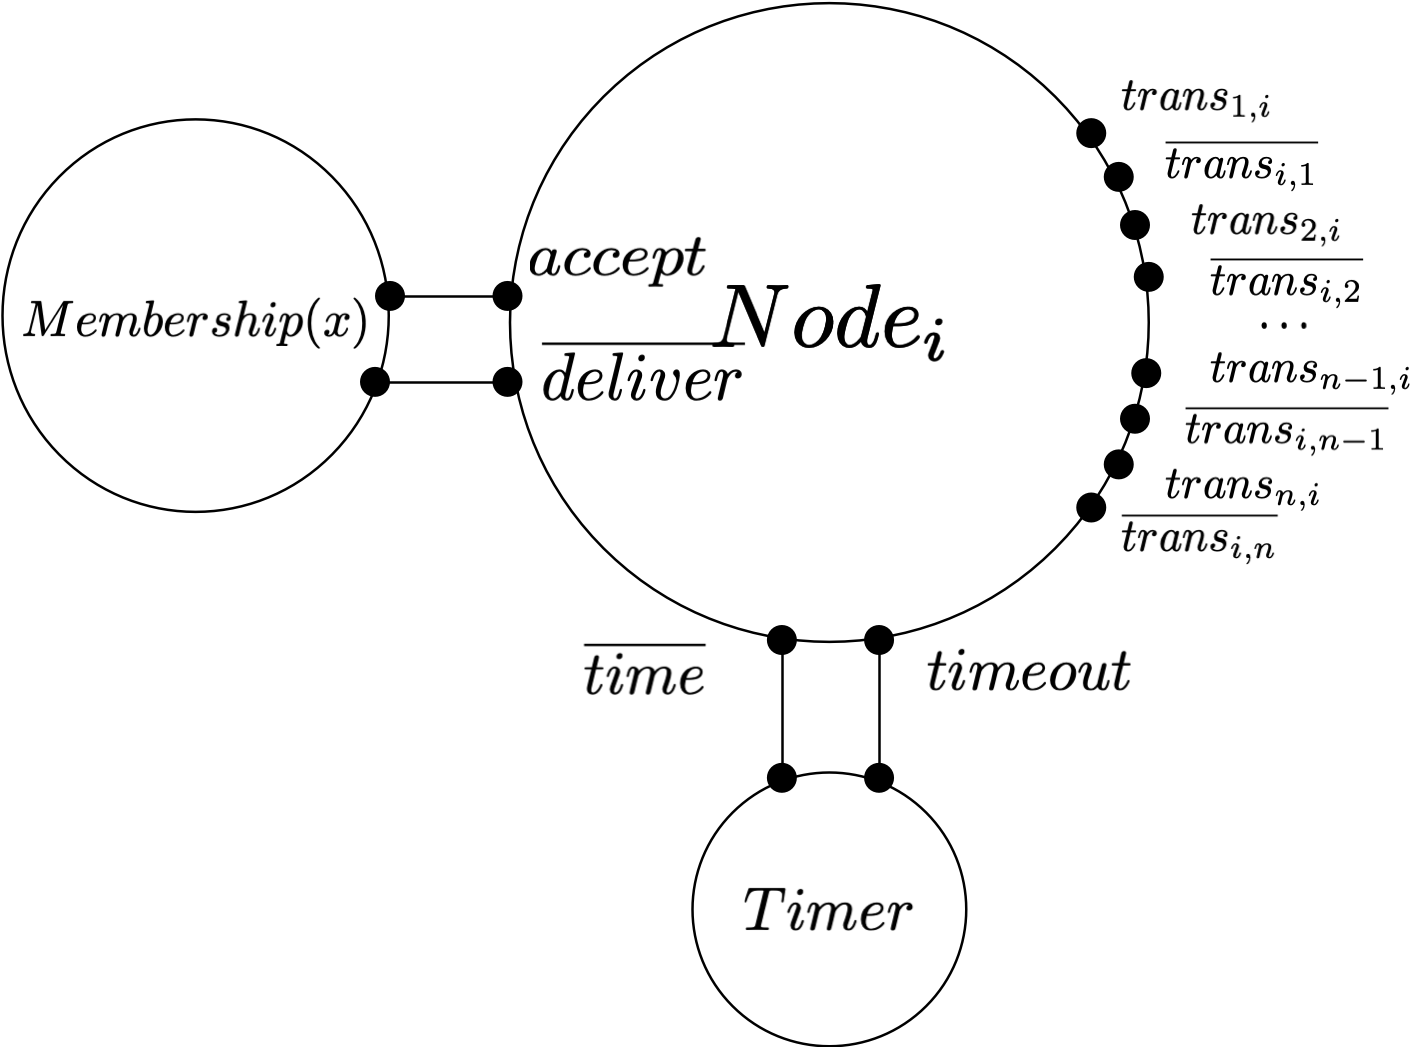
\includegraphics[width=6cm]{../figures/Node.png}
    \caption{\textbf{Gossip-Style Membership Protocol 节点示意图}}
    \label{fig:membership_node}
\end{figure}

Gossip-Style Membership协议中的P2P系统定义如下,
\begin{align*}
    FragileNode_i&\stackrel{def}{=}p_{fail}\tau.BadNode_i\oplus (1-p_{fail})\tau.Node_i\\
    BadNode_i&\stackrel{def}{=}\tau.FragileNode_i\\
    Node_i&\stackrel{def}{=}timeout.accept(x).(\bigoplus_{perm\in \mathsf{PERM}_i} p_{perm}\tau.GossipingNode_{i,perm}(x))\\
     &+\sum_{j\in \mathsf{N}/\{i\}}trans_{j,i}(x).\overline{deliver}(x).FragileNode_i\\
    GossipingNode_{i,perm}(x)&\stackrel{def}{=}\overline{trans_{i,perm_{1}}}(x).\dots \overline{trans_{i,perm_{b}}}(x).\overline{time}.FragileNode_i\\
    GossipSystem_\mathsf{N}&\stackrel{def}{=}(FragileNode_1\mid FragileNode_2\mid \dots \mid FragileNode_n)\\
    &\backslash \{trans_{i,j}\mid i\in \mathsf{N} \wedge j\in \mathsf{N} \wedge i\neq j\}\cup \{time, timeout, accept, deliver\}
 \end{align*}
 其中,每一个节点定义为$FragileNode$,每一时刻
 它会有$p_{fail}$的概率成为失效节点$BadNode$,
 和$1-p_{fail}$的概率成为可发送列表和接受列表的正常节点$Node$。
 在$Node$状态的节点,
 可以在外界计时器发送$timeout$信号时通过$accept$通道获取自身的
 Membership List,
 以概率$p_{\mathsf{perm}}$
 的概率选定$\mathsf{N}/\{i\}$中任选$\mathsf{k}$个元素的全排列
 中的一个排列$perm$作为发送目标,
 进而迁移为$GossipingNode_{i,perm}(x)$,
 向$perm$中的节点发送Membership List,
 发送完成后回到$FragileNode$的状态。
 一个有$n=|\mathsf{N}|$个节点的
 基于Gossip-Style Membership协议的P2P系统定义为
 $GossipSystem_{\mathsf{N}}$,
 它由$n$个$FragileNode$状态的并发的节点构成。

 此外,我们还需要定义每个节点本地的Membership系统,
 来处理Membership List的获取和更新。
 Membership List的内容一般为表~\ref{tab:membership_list}中的内容。
\begin{table}[!hpt]
    \caption[Membership List]{Membership List}
    \label{tab:membership_list}
    \centering
    \begin{tabular}{@{}ccc@{}} \toprule
    %   \multicolumn{2}{c}{Item} \\ \cmidrule(r){1-2}
      Address & HeartBeat & LocalTime \\ \midrule
      1 & 10120 & 66\\
      2 & 10103 & 62\\
      3 & 10098 & 63\\ \bottomrule
    \end{tabular}
  \end{table}
其中Address表示系统中其他节点的地址,HeartBeat表示对应节点的心跳计数,
LocalTime表示Membership List中这一项记录最近一次的更新时间,
当当前时间与某一项的LocalTime相差超过$T_{fail}$,
我们认为这一节点失效。

因此Membership系统需要有一个本地计时器Timer、一个心跳计数器Counter,
一个本地$MembershipList(X)$,
$X$应为一个(Address, HeartBeat, LocalTime)
的三元组的数组,
一个记录本地地址的$AddrInfo(address)$
(地址应在加入网络时由DNS分配,此处不考虑它的分配过程)。
定义$x_i[Address]$为取Address的值的操作子,
$x_i[HeartBeat]$同理。
$n$为MembershipList的最大容量。

我们定义的Membership系统的实现如图~\ref{fig:membership_system}所示,
\begin{figure}[!htbp]
	\small
	\centering
	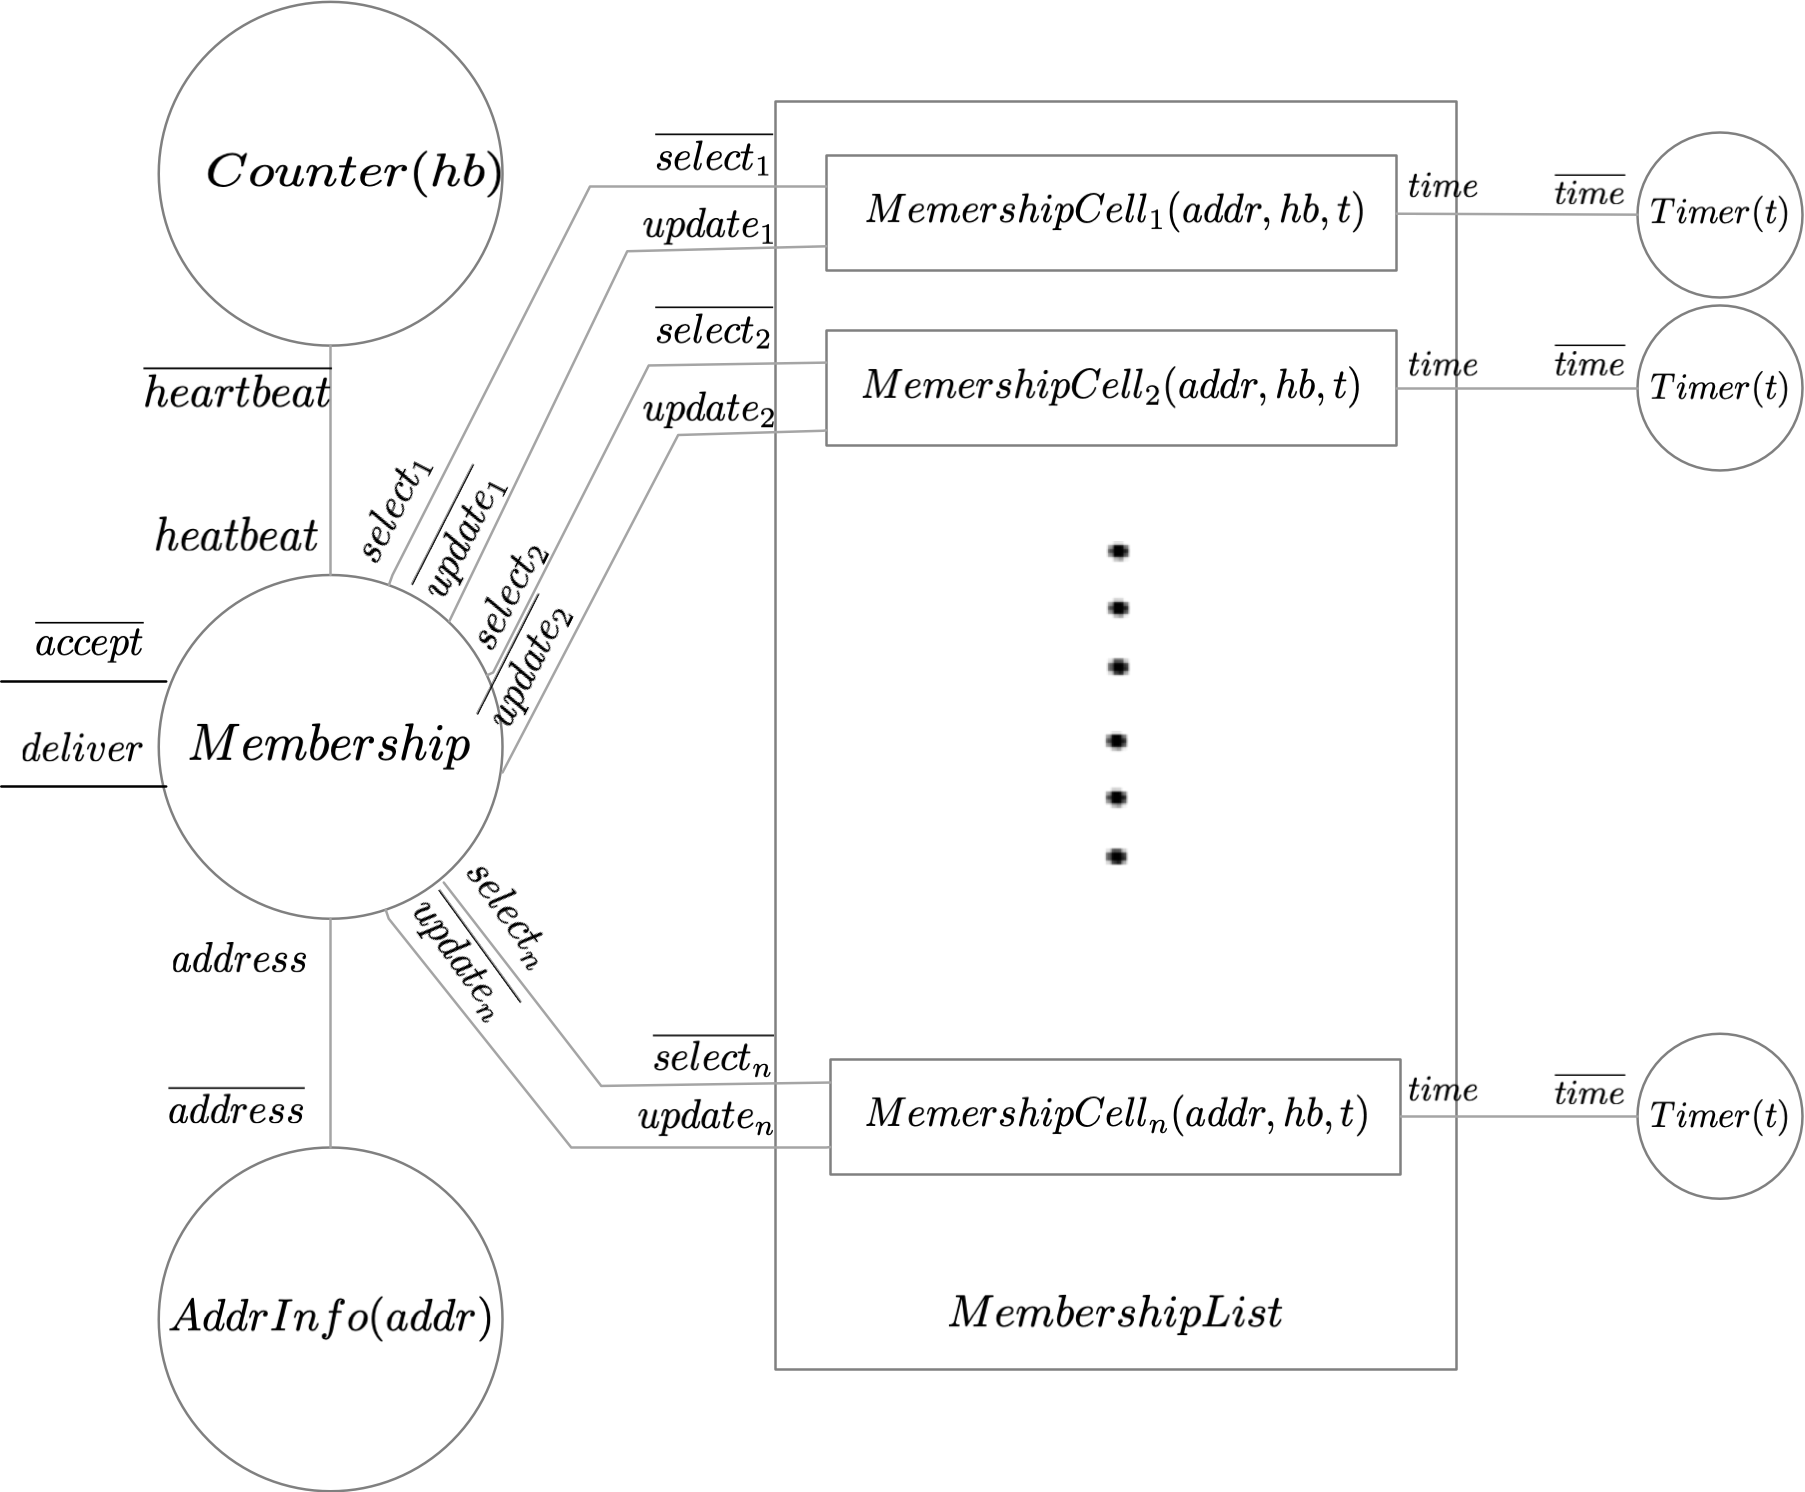
\includegraphics[width=11cm]{../figures/membership.png}
    \caption{\textbf{Membership示意图}}
    \label{fig:membership_system}
\end{figure}
可以看到,我们使用$n$个$MembershipCell$来存储Membership List中的每一项,
$Membership$可以通过$select_i$通道获取$MembershipCell_i$中的数据,
也可以通过$update_i$通道更新$MembershipCell_i$中的数据,
每一个$MembershipCell$连接一个Timer,用来获取本地时间,设置LocalTime字段,
实际上,对于一个节点它可能只有一个Timer,这里的连接也是指逻辑连接。
$MembershipCell$的定义如下:
\begin{align*}
   &MembershipCell_i(addr,hb,t)\stackrel{def}{=}\\
   &\quad\overline{select_i}(\{Address:addr,HeartBeat:hb\}).MembershipCell_i(addr,hb,t)\\
   &\quad+update_i(\{Address:addr',HeartBeat:hb'\}).time(t').MembershipCell_i(addr',hb',t')
\end{align*}
$n$个$MembershipCell$组成的$MembershipList$定义如下,在初始状态时,每一个$MembershipCell$中的数据为空($\epsilon$):
\begin{align*}
   MembershipList\stackrel{def}{=}(MembershipCell_1(\epsilon)\mid \dots MembershipCell_n(\epsilon))
\end{align*}

此外,我们定义了一个$Counter$维护和更新节点的心跳,
在每一次Gossip周期$hb=hb+1$,
$Membership$可以通过$heartbeat$通道获取心跳。
\begin{align*}
   Counter(hb)\stackrel{def}{=}\overline{heartbeat}(\mathsf{s}(hb)).Counter(\mathsf{s}(hb))
\end{align*}
对于节点本地地址的维护,我们定义了一个$AddrInfo$,
$Membership$可以通过$address$通道获取本地地址。
\begin{align*}
   AddrInfo(addr)\stackrel{def}{=}\overline{address}(addr)
\end{align*}

定义完以上的辅助工具后,我们可以定义$Membership$的逻辑了!
\begin{align*}
    &Membership\stackrel{def}{=}address(addr).heartbeat(hb).select_1(x_1)\dots select_n(x_n).\\
    &\quad\overline{accept}(\{Address:addr,HeartBeat:hb\},x_1,\dots,x_n).Membership\\
    &\quad+deliver(x_1,x_2,\dots,x_n).Processing(x_1,x_2,\dots,x_n)\\
    &Processing(x_1,x_2,\dots,x_n)\stackrel{def}{=}(Check(x_1)\mid  \dots \mid Check(x_n) \mid Membership)\\
    &Check(x)\stackrel{def}{=}address(addr).((addr=x[Address])0|\urcorner(addr=x[Address])FindAndUpdate_1(x))\\
    &FindAndUpdate_i(x)\stackrel{def}{=}select_i(x_i).(\\
    &\quad(x_i = \epsilon) (\overline{update_i}(x).0)\\
    &\quad| \urcorner(x_i = \epsilon)(\\
    &\quad(x_i[Address]=x[Address])(\\
    &\quad(x_i[HeartBeat]<x[HeartBeat])(\overline{update_i}(x).0)\\
    &\quad\mid \urcorner (x_i[HeartBeat]<x[HeartBeat])0)\\
    &\quad\mid \urcorner (x_i[Address]=x[Address])FindAndUpdate_{i+1}(x))),i\leq n\\
    &FindAndUpdate_i(x)\stackrel{def}{=}0,i>n
\end{align*}
其中$\mathsf{s}(x)$表示$\mathsf{s}(x)=x+1$。

$Membership$可以获取$MembershipList$中所有Cell中储存的信息,
添加本地地址和心跳后,将这一组信息经$accept$通道发出,
根据$Node$的定义,我们知道$Node$从$accept$通道接受这些信息后会随机的发送给$k$个其他节点。
另外,$Membership$从$deliver$通道接收了其他节点发送的Membership List后,
将迁移到状态$Processing(x_1,x_2,\dots,x_n)$。
$Processing(x_1,x_2,\dots,x_n)$可以并发的运行$Check(x_i)$,
在$Check(x_i)$状态下,
若$x_i$的地址为当前节点的地址,不做处理,
若不为当前节点的地址,
则从第一个$MembershipCell$开始对比$x_i$的地址与$MembershipCell$的地址,
若地址相同且$x_i$中的心跳计数大于$MembershipCell$中的心跳计数,
更新$MembershipCell$的数据;
若所有有值的$MembershipCell$均无$x_i$的地址,用$x_i$直接更新第一个空的Cell。

\section{Gossip-Style Membership的仿真模拟}
在本节我们会根据本章的模型来实现一个基于Gossip-Style Membership Protocol的P2P系统,
由于资源限制,不能实际部署在多个主机构成的集群,我们将使用多进程来模拟多个主机,
实际上进程理论本就是用来刻画进程的并发,多个主机上的程序的本质也是进程。

\subsection{Go语言与CSP}
我们将使用Go语言实现Gossip-Style Membership Protocol,
Go语言实现了两种并发模型,一种是C++,Java使用的多线程,一种是CSP并发模型。
如我们在第~\ref{ch:intro}章中提到的,
CSP也是一种经典的进程演算,它与CCS的区别在于等价的类型和建模并发系统采用的方法,有关CCS和CSP对比的研究也有很多[cite3]。
Go语言使用了CSP理论中的Process/Channel,对应到语言中的 goroutine/channel。[cite2]
Goroutine是一种轻量级线程,channel用于协程间的通信。
我们使用Go语言的并发特性可以更加直观的展示出对前述模型的代码实现。

% CSP也是一种进程演算,
% 与CCS存在相似和差异[cite],
% 本实现主要利用了Go语言的通道特性,
% 通道的概念是CSP的组成部分,
% 在CCS中对应端口的概念,其本质是相似的。
% 使用Go语言的通道可以更加直观的展示出对上述模型的代码实现。

\subsection{代码实现与仿真效果}

 由于代码的解释比较枯燥,本小节只展示关键部分的代码实现,
 完整的代码实现及下载、运行方式可以参考附录~\ref{app:code}。
 在编写代码的过程中,考虑到代码的可读性和字符的限制,
 我们对前述模型通道和进程状态的名称有所修改,
 但本质没有变化。

 在Go语言中,我们可以用channel特性来实现$\mathbb{RVPC}_{\mathsf{Th}}$中的通道。
 如在实现Gossip-Style Membership协议的节点结构时,
 Node结构体中,chan类型的字段分别
 代表了图~\ref{fig:membership_node}中的相应名字的通道。
 其中,我们在~\ref{ch:gossip_impl}小节中提到
 $trans_{i,j}$通道用于节点$i$向节点$j$传输信息,
 这一通道实质上表达的是信息传输的逻辑路径,
 我们在实现时考虑信息传输的代码层面的物理路径,
 只需要每一个节点设置一个
 $trans$通道用于接收集群中其他节点的信息即可,
 向其他节点发送信息时,我们可以通过Others字段向
 Others[i].trans通道发送消息。
 对于Node节点的状态迁移,我们可以使用bool类型的字段isbad表示节点状态是否为BadNode。
 \begin{codeblock}[language=GO]
   type Node struct {
      isbad bool
      trans chan []Message
      time chan Nil
      timeout chan Nil
      accept chan []Message
      deliver chan []Message
      Others []*Node
   }
\end{codeblock}

我们可以使用基于select的多路复用实现非确定性选择,
如我们在~\ref{ch:membership_system}中实现的系统中的:
\begin{align*}
   Node_i&\stackrel{def}{=}timeout.accept(x).(\bigoplus_{perm\in \mathsf{PERM}_i} p_{perm}\tau.GossipingNode_{i,perm}(x))\\
     &+\sum_{j\in \mathsf{N}/\{i\}}trans_{j,i}(x).\overline{deliver}(x).FragileNode_i
\end{align*}
这里$Node_i$可以做非确定的选择:
接收到timeout信号后从accept通道获取本地的Membership List
随机选择$k$个其他节点发送;或从其他节点接收到Membership List消息,
通过deliver通道向本地的Membership进程传递该消息。

\begin{codeblock}[language=GO]
   select {
      //timeout.accept(x).bigoplus p tau.GossipingNode
      case <- node.timeout:
         messages := <- node.accept
         //随机生成k个其他节点的排列targets
         node.Gossiping(messages, targets)
      // sum trans(x).deliver(x).FragileNode
      case message := <- node.trans:
         node.deliver <- message
	}
\end{codeblock}
select的语法与switch比较相似,
每一个case代表一个通信操作,
select会等待case中有能够执行的case时执行该case:
当条件满足时,select才会通信并执行case后的语句块,
其他通信不执行。

在Go语言中,每一个并发执行的单元称为一个goroutine,
我们同样使用goroutine来实现$\mathbb{RVPC}_{\mathsf{Th}}$
中的并发。
如对$GossipSystem_\mathsf{N}\stackrel{def}{=}(FragileNode_1\mid FragileNode_2\mid \dots \mid FragileNode_n)$,
的实现:
\begin{codeblock}[language=GO]
   for i:=0;i<NODE_NUM;i++ {
        go nodes[i].Fragile()
    }
\end{codeblock}
实际上在我们的系统中,对一个节点本地的Timer,Membership和接入通信网络的Node
同样应该是并发的。

本节仿真实现的基于Gossip-Style Membership协议的P2P系统参数如表~\ref{tab:param}。
\begin{table}[!hpt]
   \caption[基于Gossip-Style Membership协议的P2P系统]{基于Gossip-Style Membership协议的P2P系统}
   \label{tab:param}
   \centering
   \begin{tabular}{@{}ccc@{}} \toprule
   %   \multicolumn{2}{c}{Item} \\ \cmidrule(r){1-2}
     参数名称 & 参数值 & 参数含义 \\ \midrule
     $n$ & 5 & 系统节点数量\\
     $k$ & 2 & 每Gossip周期发送的节点数\\
     $p_{fail}$ & 0.1 & 节点失效概率\\ \bottomrule
   \end{tabular}
 \end{table}

 我们使用上述参数运行我们实现的系统,
 我们使用html为我们的系统做了一个前端界面,
 我们可以在这个界面观察每个节点Membership List的更新过程。

 \begin{figure}[!htp]
   \begin{minipage}{0.9\textwidth}
     \centering
     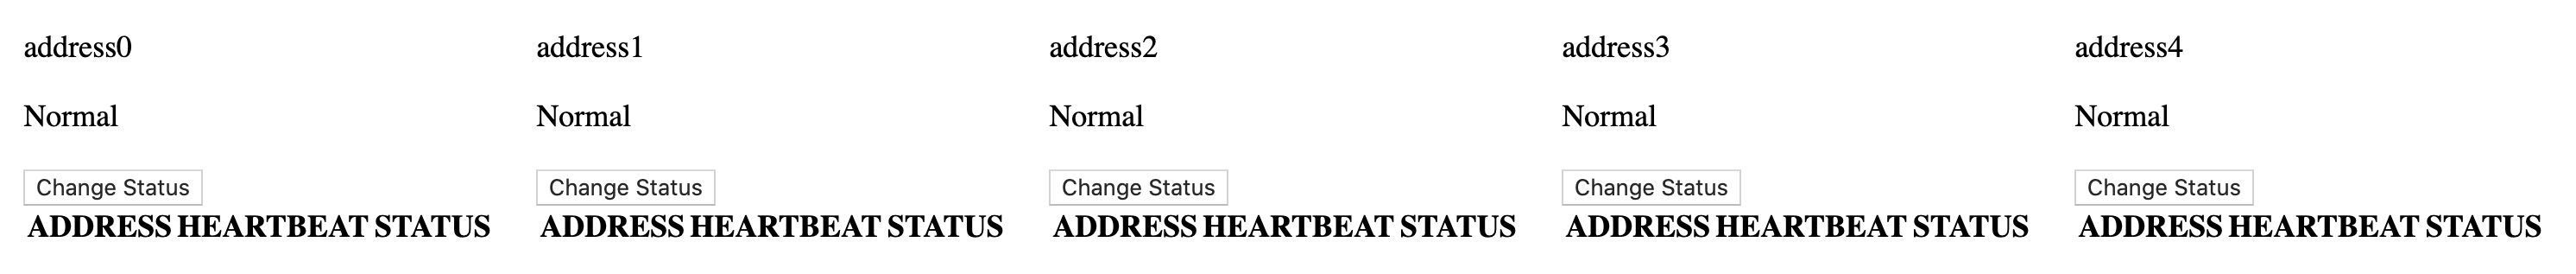
\includegraphics[width=15cm]{../figures/demo/4.png}
     \\
     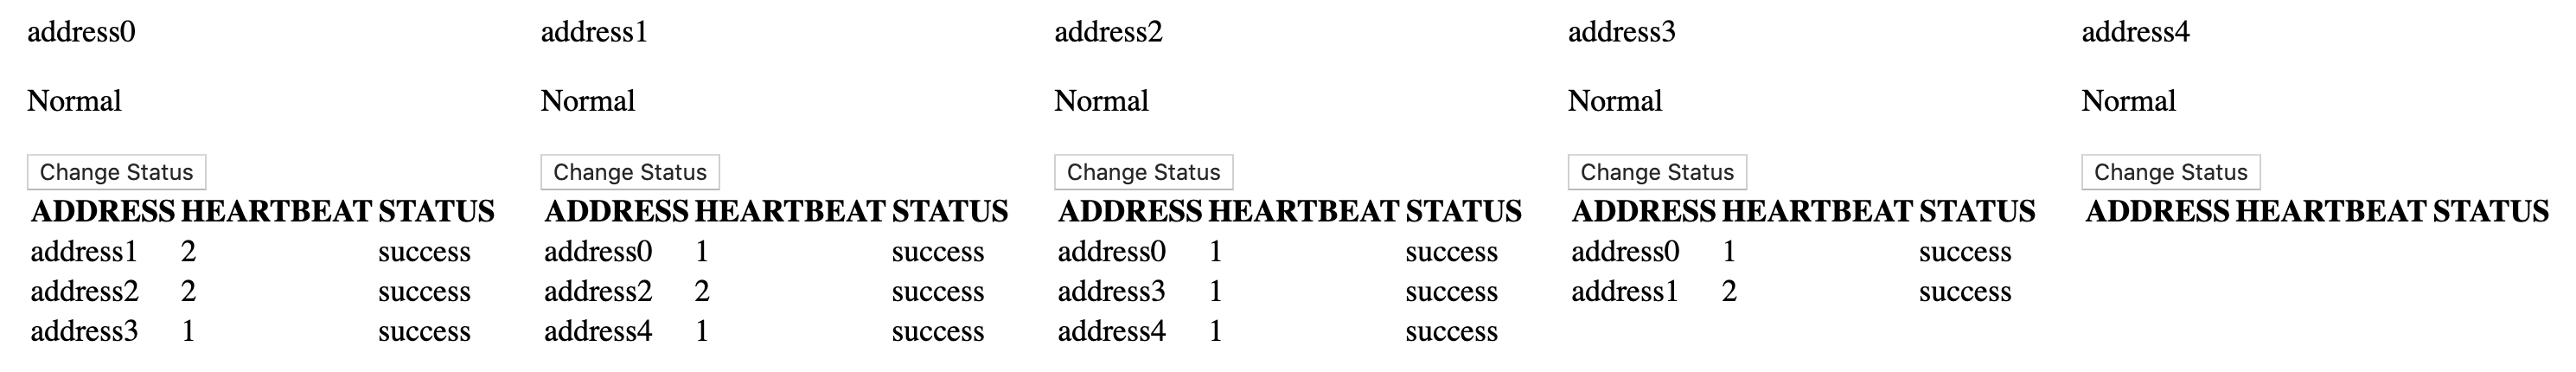
\includegraphics[width=15cm]{../figures/demo/5.png}
     \\
     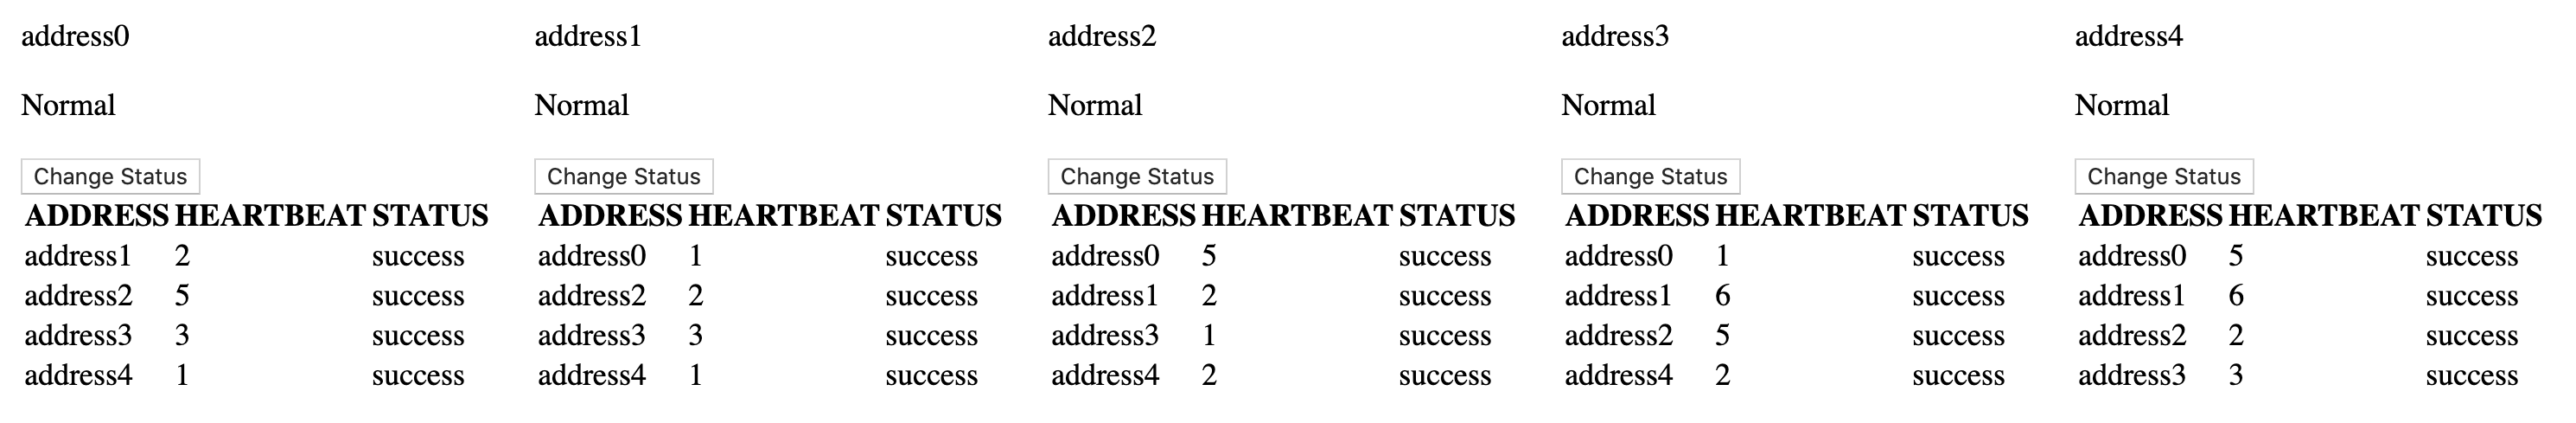
\includegraphics[width=15cm]{../figures/demo/6.png}
   \end{minipage}
   \caption{基于Gossip-Style Membership协议的5节点P2P系统的Membership List扩展过程}
   \label{fig:demo_1}    
\end{figure}
 图~\ref{fig:demo_1}展示了每个节点的Membership List的扩展过程,
 其中第一行为节点的地址,我们使用字符串表示,也可以根据需要修改成其他的形式,
 第二行为对应节点的状态,Bad表示节点失效,对应$BadNode$状态,
 Normal表示节点正常,对应$FragileNode$和$Node$状态,
 第三行的按钮可以改变节点的状态,
 接下来的是对应节点的Membership List,可以看到我们展示了Address,Heartbeat, Status字段,
 其中Status字段是由LocalTime计算而得,
 当当前时间与Membership List项的LocalTime字段相差超过$T_{fail}$时,我们认为这一项对应的节点处于失效状态。
 在~\ref{fig:demo_1}的第一个图中,我们可以看到初始状态所有节点的Membership List为空,
 第二张图中Membership List进行了扩张,第三张图中全部节点的Membership List包含了所有其他节点。

我们同样可以展示系统的失效检测。在图~\ref{fig:demo_2}中,
第一张图是正常状态,
我们在第二张图中手动改变了地址为address1节点状态,使该节点失效,
可以看到第三张图中address0,address3检测到了address1的失效,
第四张图所有节点都检测到了address1的失效。
 \begin{figure}[!htp]
   \begin{minipage}{0.9\textwidth}
     \centering
     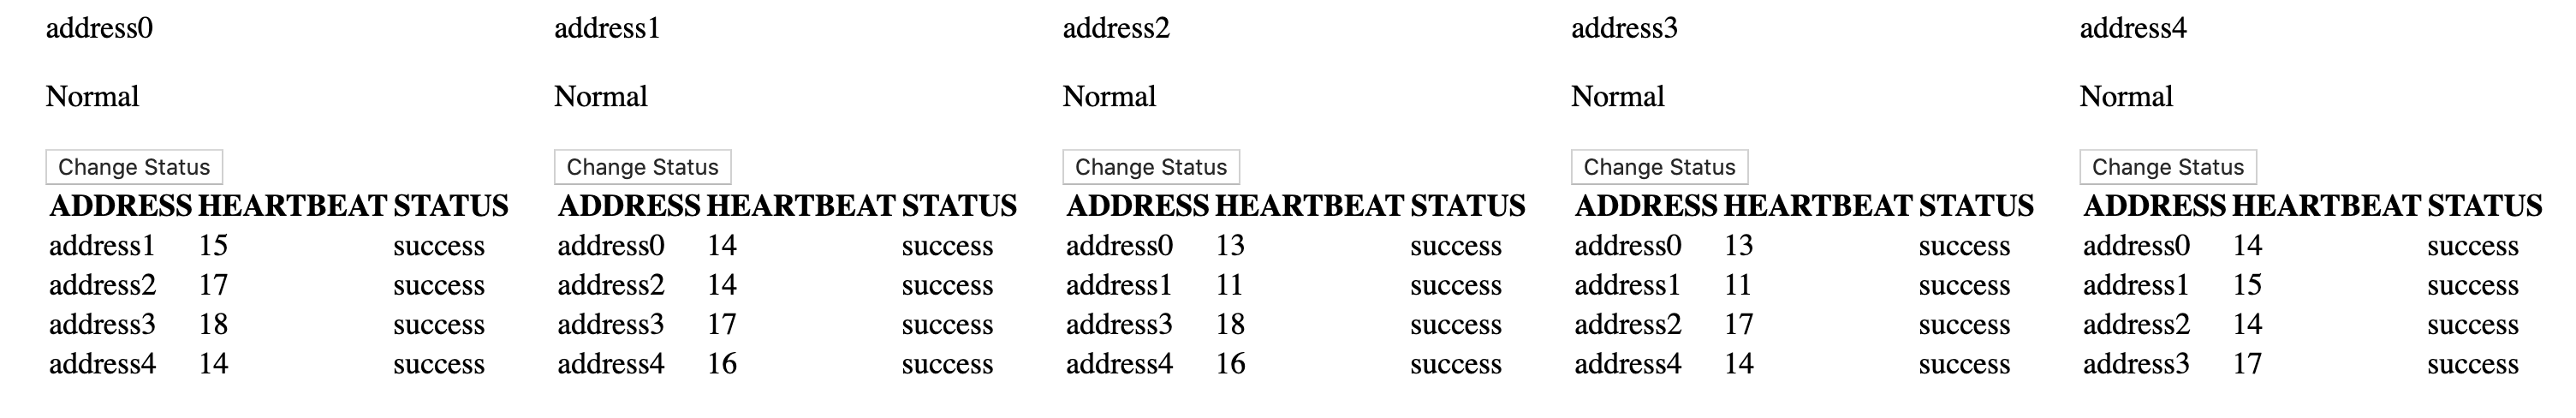
\includegraphics[width=15cm]{../figures/demo/0.png}
     \\
     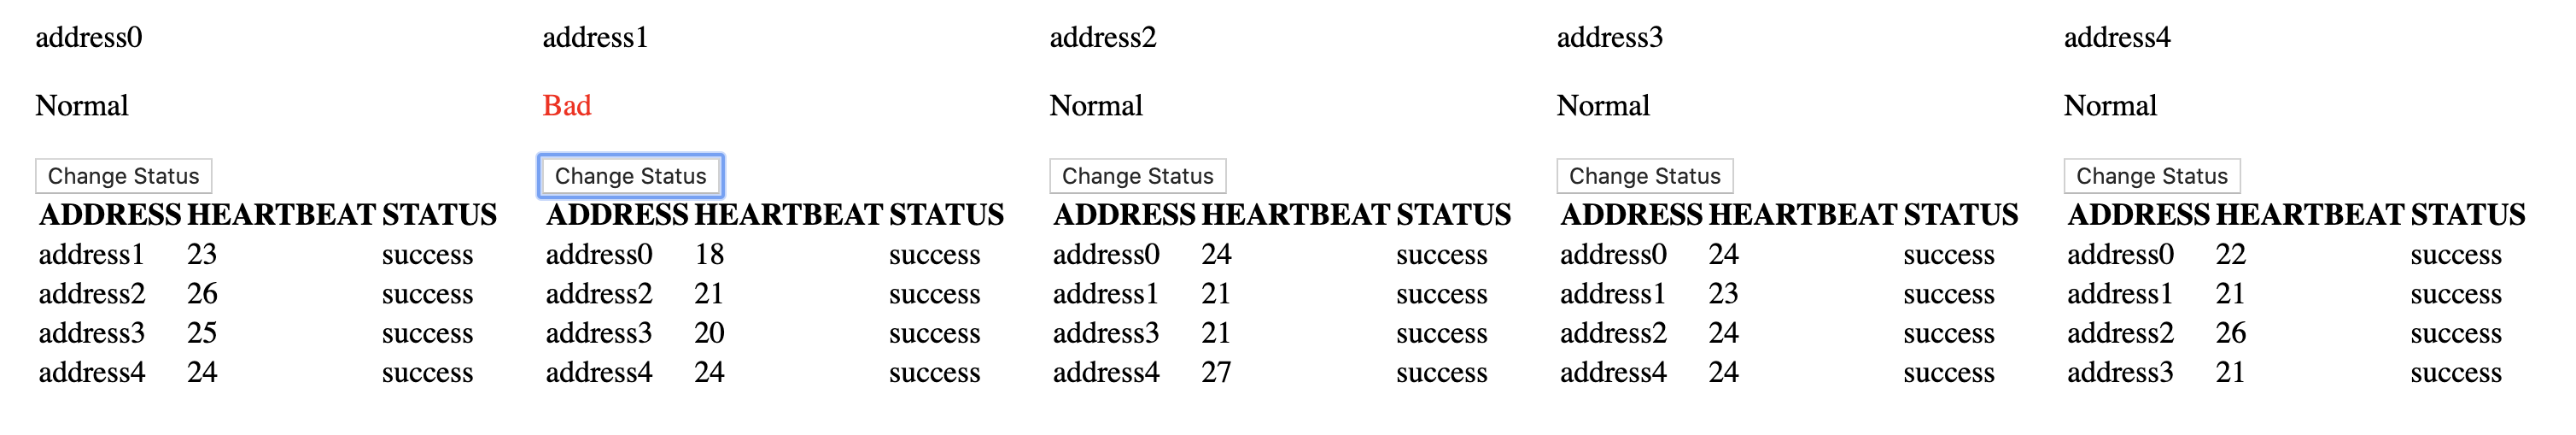
\includegraphics[width=15cm]{../figures/demo/1.png}
     \\
     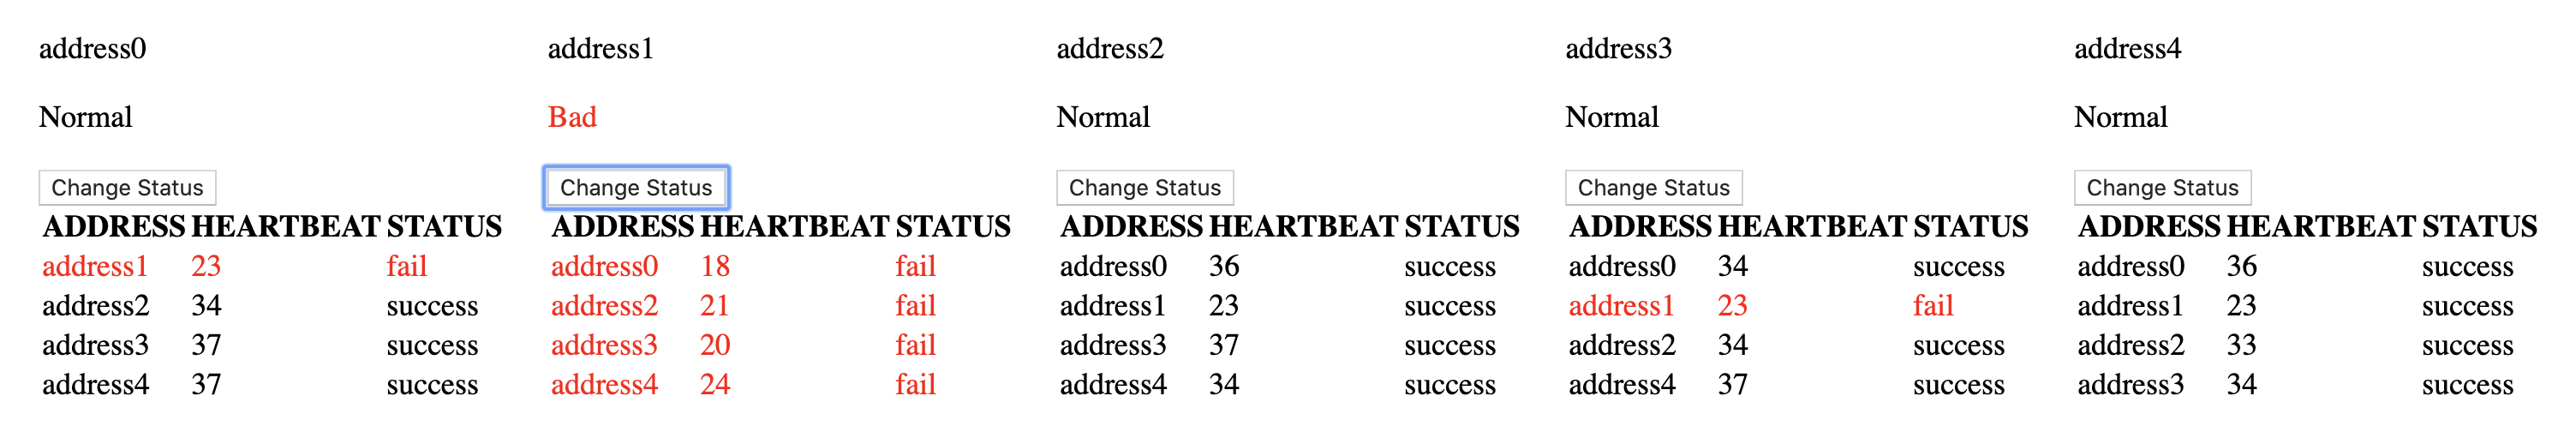
\includegraphics[width=15cm]{../figures/demo/2.png}
     \\
     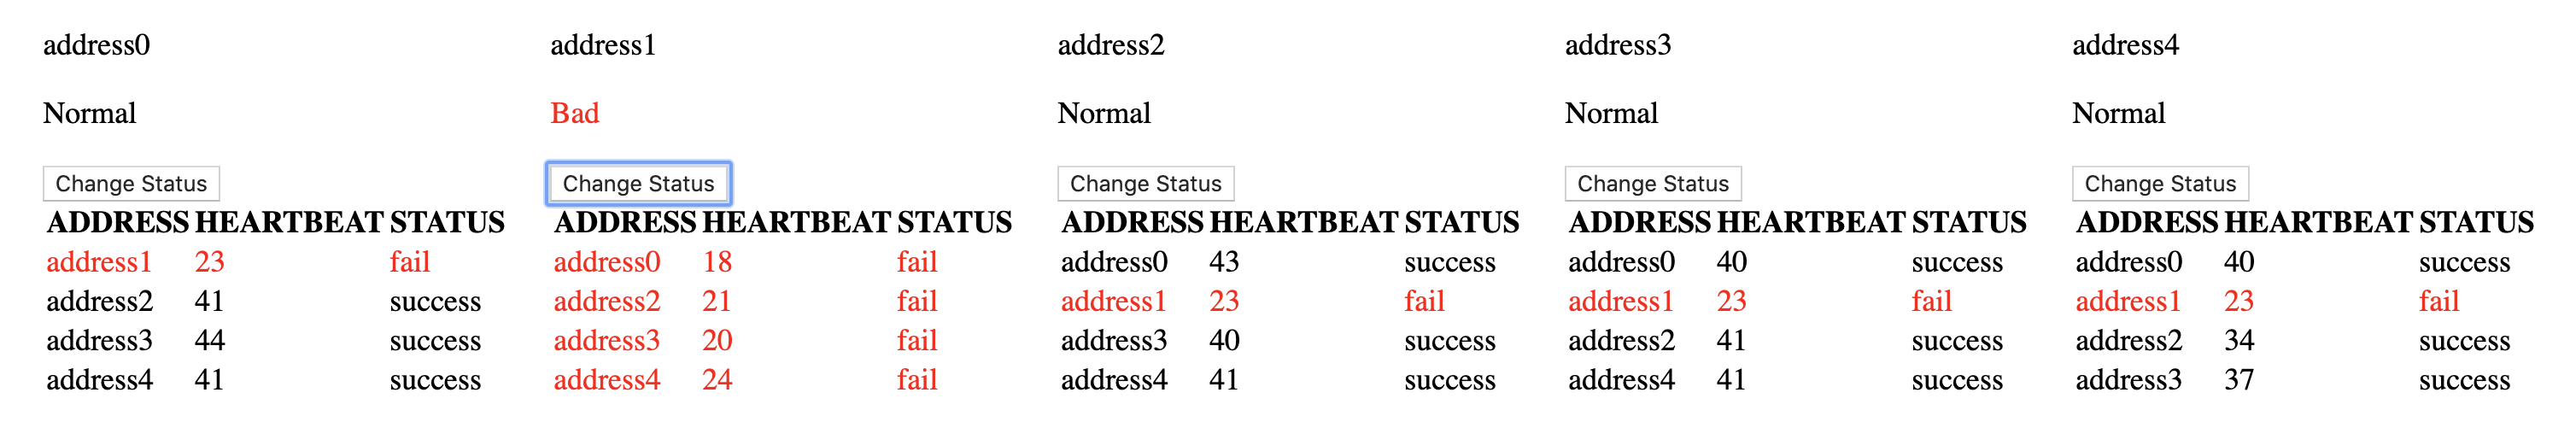
\includegraphics[width=15cm]{../figures/demo/3.png}
   \end{minipage}
   \caption{基于Gossip-Style Membership协议的5节点P2P系统的错误检测}
   \label{fig:demo_2}   
\end{figure}

我们也可以通过设置$p_{fail}$使系统中的节点以一定概率自动失效和恢复,
动态效果可以通过附录~\ref{app:code}中的方式获得。

 \section{本章小结}
 本章我们以一种云计算失效检测协议Gossip-Style Membership协议的
 $\mathbb{RVPC}_{\mathsf{Th}}$实现作为
 本文中提出的随机传值进程模型的应用,
 提供了使用$\mathbb{RVPC}_{\mathsf{Th}}$建模及实现通信协议以至其他现实问题的思路。

 我们首先介绍了Gossip协议和Membership协议,
并使用$\mathbb{RVPC}_{\mathsf{Th}}$实现了基于Gossip协议的P2P系统,
使用$\mathbb{RVPC}_{\mathsf{Th}}$的符号互模拟证明了Gossip协议与多播规约的观察等价性。
在基于Gossip协议的P2P系统的基础上,我们修改实现使其成为基于
Gossip-Sytle Membership协议的P2P系统,并给出了GO语言的代码实现和仿真模拟。

% !TEX root = ../main.tex
\chapter{总结与展望}

随着随机和交互在现代计算机科学中的应用日渐广泛,
概率进程模型的研究也备受关注。
而作为适用范围颇为广泛的一种经典进程模型,
传值进程模型的概率扩展也有很多研究。
在已有工作中,对传值进程模型的扩展往往局限于某一个特定的应用场景,
或因为作为基础的传值进程模型的局限性,其模型完整性尚有欠缺,
普遍意义上的概率传值进程模型的研究尚显不足。
本文致力于在已有的通用概率扩展方法和传值进程模型的基础上
探索具有普适性的传值进程模型的概率扩展。

本文在传值进程模型$\mathbb{VPC}_{\mathsf{Th}}$的基础上,
使用一种模型无关的概率扩展方法,
扩展了$\mathbb{VPC}_{\mathsf{Th}}$的语法和迁移语义,
增加了随机选择操作子,
使其除非确定性选择之外还可以做随机选择,
我们称这一模型为随机传值进程模型,记为$\mathbb{RVPC}_{\mathsf{Th}}$。

同时,为了给出$\mathbb{RVPC}_{\mathsf{Th}}$的观察等价性的定义,
我们使用Uniform Approach的方法定义了条件等价集、条件等价树(森林)、
条件$l$转移和条件$q$转移,进而定义了$\mathbb{RVPC}_{\mathsf{Th}}$下
的符号互模拟。
在Uniform Apprach中,
条件等价树的本质是概率化了$\mathbb{VPC}_{\mathsf{Th}}$中的
状态保持的静态迁移$A\Rightarrow_{\varphi}A'=A$,
$\mathbb{RVPC}_{\mathsf{Th}}$中的符号互模拟的本质是
用条件等价树中条件$\varphi$对应的划分$\{\varphi_i\}_{i\in I}$所
对应的条件等价森林模拟条件等价树中的条件$l$转移和条件$q$转移。
我们将共发散的符号互模拟关系的全集定义为$\mathbb{RVPC}_{\mathsf{Th}}$的观察等价性,
并给出了观察等价性的同余性证明。

最后,我们以一种云计算协议Gossip-Style Membership Protocol为例,
给出了使用$\mathbb{RVPC}_{\mathsf{Th}}$建模通信过程,乃至其他现实问题的
方法和过程,并使用$\mathbb{RVPC}_{\mathsf{Th}}$的符号互模拟
给出了Gossip协议与我们定义的多播规约的观察等价性。
给出Gossip-Style Membership Protocol的模型的同时,
我们使用Go语言实现了这个模型,并分析了Go语言特性对应
部分$\mathbb{RVPC}_{\mathsf{Th}}$操作子的实现。
事实证明$\mathbb{RVPC}_{\mathsf{Th}}$在建模和分析通信过程时具有一定的可行性。
我们希望$\mathbb{RVPC}_{\mathsf{Th}}$可以为
含有传值、计算性质的现实问题的建模和分析提供有效、可行的方法。

然而,目前的模型仍有一定的不足,
我们认为下一步的研究工作主要可以从以下几个方面入手:

第一,随机传值进程模型中的随机性可以体现在两个方面:\textit{内容随机性}和\textit{通道随机性},
内容随机性体现在值的随机性,外界向进程传的值可能会在某一个值域中符合某种概率分布,或近似符合某种概率分布;
而通道随机性体现在进程对通信通道的选择是随机的,如在第~\ref{ch:gossip}章中,Gossip协议会周期性的随机选择通信的对象。
由于Uniform Approach中只关注了通道的随机性,
在本文对随机传值进程模型的定义中,我们也只关注了通道的随机性。
这样做有一定的合理性:对于一个与具体问题无关的形式化方法,
我们无法给定值的一个具体的随机分布。
对于具体的问题,我们可以在$\mathbb{RVPC}_{\mathsf{Th}}$的基础上考虑值的随机分布。

但遗憾的是,
在第~\ref{ch:gossip}章中我们给出的应用,
包括在第~\ref{ch:rvpc}章中的简单的例子,
实际上都是$\mathbb{RVPC}_{\mathsf{Th}}$
上的\textit{进程},
由于系统没有与外界的值的通信,整个系统中没有自由变元,
因此依旧是不需要考虑内容随机性的模型。
这是本文在构思上一个欠考虑的地方,
实际上建模一个与外界有值传递的系统对于本文的意义会更大一些。
进一步的研究可以关注内容随机性。
对于内容的随机性的实现,MILNER R在Communication and Concurrency\cite{Milner_CCS}
中在将书中的提供了一个思路:
为了建模传值的CCS,MILNER R将Value-passing CCS转化为CCS时
将$S=a(x).T$转为$S=\sum_{v\in V} a_v.T\{v/x\}$,其中$V$是给定值的集合。
我们也可以用$S=\bigoplus_{v\in V}p_v.\tau.a(v).T\{v/x\}$的方法来建模值的随机性。

第二,我们希望本文提出的随机传值进程模型也是一种通用的模型,
不只局限于本文第~\ref{ch:gossip}章中的应用场景,
甚至不局限于通信过程的建模,
而是能够适用于很多具有传值特点的并发过程。
我们希望应用场景甚至可以是跨学科的,包括生物过程、生产流程等等。
进一步的工作也可以是在这些领域中使用随机传值进程模型解决一些问题。

% % !TEX root = ../thesis.tex

\chapter{简介}

这是 \sjtuthesis 的示例文档,基本上覆盖了模板中所有格式的设置。建议大家在使用模
板之前,除了阅读《\sjtuthesis\ 使用文档》,这个示例文档也最好能看一看。

\section{二级标题}

\subsection{三级标题}

\subsubsection{四级标题}

Lorem ipsum dolor sit amet, consectetur adipiscing elit, sed do eiusmod tempor
incididunt ut labore et dolore magna aliqua. Ut enim ad minim veniam, quis
nostrud exercitation ullamco laboris nisi ut aliquip ex ea commodo consequat.
Duis aute irure dolor in reprehenderit in voluptate velit esse cillum dolore eu
fugiat nulla pariatur. Excepteur sint occaecat cupidatat non proident, sunt in
culpa qui officia deserunt mollit anim id est laborum.

\section{脚注}

Lorem ipsum dolor sit amet, consectetur adipiscing elit, sed do eiusmod tempor
incididunt ut labore et dolore magna aliqua. \footnote{Ut enim ad minim veniam,
quis nostrud exercitation ullamco laboris nisi ut aliquip ex ea commodo
consequat. Duis aute irure dolor in reprehenderit in voluptate velit esse cillum
dolore eu fugiat nulla pariatur.}

\section{字体}


上海交通大学是我国历史最悠久的高等学府之一,是教育部直属、教育部与上海市共建的全
国重点大学,是国家“七五”、“八五”重点建设和“211 工程”、“985 工程”的首批建
设高校。经过 115 年的不懈努力,上海交通大学已经成为一所“综合性、研究型、国际化”
的国内一流、国际知名大学,并正在向世界一流大学稳步迈进。 

{\songti 十九世纪末,甲午战败,民族危难。中国近代著名实业家、教育家盛宣怀和一批
  有识之士秉持“自强首在储才,储才必先兴学”的信念,于 1896 年在上海创办了交通大
  学的前身——南洋公学。建校伊始,学校即坚持“求实学,务实业”的宗旨,以培养“第
  一等人才”为教育目标,精勤进取,笃行不倦,在二十世纪二三十年代已成为国内著名的
  高等学府,被誉为“东方MIT”。抗战时期,广大师生历尽艰难,移转租界,内迁重庆,
  坚持办学,不少学生投笔从戎,浴血沙场。解放前夕,广大师生积极投身民主革命,学校
  被誉为“民主堡垒”。}

{\heiti 新中国成立初期,为配合国家经济建设的需要,学校调整出相当一部分优势专业、
  师资设备,支持国内兄弟院校的发展。五十年代中期,学校又响应国家建设大西北的号
  召,根据国务院决定,部分迁往西安,分为交通大学上海部分和西安部分。1959 年 3月
  两部分同时被列为全国重点大学,7 月经国务院批准分别独立建制,交通大学上海部分启
  用“上海交通大学”校名。历经西迁、两地办学、独立办学等变迁,为构建新中国的高等
  教育体系,促进社会主义建设做出了重要贡献。六七十年代,学校先后归属国防科工委和
  六机部领导,积极投身国防人才培养和国防科研,为“两弹一星”和国防现代化做出了
  巨大贡献。}

{\kaishu 改革开放以来,学校以“敢为天下先”的精神,大胆推进改革:率先组成教授代
  表团访问美国,率先实行校内管理体制改革,率先接受海外友人巨资捐赠等,有力地推动
  了学校的教学科研改革。1984 年,邓小平同志亲切接见了学校领导和师生代表,对学校
  的各项改革给予了充分肯定。在国家和上海市的大力支持下,学校以“上水平、创一流”
  为目标,以学科建设为龙头,先后恢复和兴建了理科、管理学科、生命学科、法学和人文
  学科等。1999 年,上海农学院并入;2005 年,与上海第二医科大学强强合并。至此,学
  校完成了综合性大学的学科布局。近年来,通过国家“985 工程”和“211 工程”的建
  设,学校高层次人才日渐汇聚,科研实力快速提升,实现了向研究型大学的转变。与此同
  时,学校通过与美国密西根大学等世界一流大学的合作办学,实施国际化战略取得重要突
  破。1985 年开始闵行校区建设,历经 20 多年,已基本建设成设施完善,环境优美的现
  代化大学校园,并已完成了办学重心向闵行校区的转移。学校现有徐汇、闵行、法华、七
  宝和重庆南路(卢湾)5 个校区,总占地面积 4840 亩。通过一系列的改革和建设,学校
  的各项办学指标大幅度上升,实现了跨越式发展,整体实力显著增强,为建设世界一流大
  学奠定了坚实的基础。}

{\fangsong 交通大学始终把人才培养作为办学的根本任务。一百多年来,学校为国家和社
  会培养了 20余万各类优秀人才,包括一批杰出的政治家、科学家、社会活动家、实业
  家、工程技术专家和医学专家,如江泽民、陆定一、丁关根、汪道涵、钱学森、吴文俊、
  徐光宪、张光斗、黄炎培、邵力子、李叔同、蔡锷、邹韬奋、陈敏章、王振义、陈竺等。
  在中国科学院、中国工程院院士中,有 200 余位交大校友;在国家 23 位“两弹一星”
  功臣中,有 6 位交大校友;在 18 位国家最高科学技术奖获得者中,有 3 位来自交大。
  交大创造了中国近现代发展史上的诸多“第一”:中国最早的内燃机、最早的电机、最早
  的中文打字机等;新中国第一艘万吨轮、第一艘核潜艇、第一艘气垫船、第一艘水翼艇、
  自主设计的第一代战斗机、第一枚运载火箭、第一颗人造卫星、第一例心脏二尖瓣分离
  术、第一例成功移植同种原位肝手术、第一例成功抢救大面积烧伤病人手术等,都凝聚着
  交大师生和校友的心血智慧。改革开放以来,一批年轻的校友已在世界各地、各行各业崭
  露头角。}

{\ifcsname lishu\endcsname\lishu\else[无 \cs{lishu} 字体。]\fi 截至 2011 年 12
  月 31 日,学校共有 24 个学院 / 直属系(另有继续教育学院、技术学院和国际教育学
  院),19 个直属单位,12 家附属医院,全日制本科生 16802 人、研究生24495 人(其
  中博士研究生 5059 人);有专任教师 2979 名,其中教授 835 名;中国科学院院士 15
  名,中国工程院院士 20 名,中组部“千人计划”49 名,“长江学者”95 名,国家杰出
  青年基金获得者 80 名,国家重点基础研究发展计划(973 计划)首席科学家 24名,国
  家重大科学研究计划首席科学家 9名,国家基金委创新研究群体 6 个,教育部创新团队
  17 个。}

{\ifcsname youyuan\endcsname\youyuan\else[无 \cs{youyuan} 字体。]\fi 学校现有本
  科专业 68 个,涵盖经济学、法学、文学、理学、工学、农学、医学、管理学和艺术等九
  个学科门类;拥有国家级教学及人才培养基地 7 个,国家级校外实践教育基地 5个,国
  家级实验教学示范中心 5 个,上海市实验教学示范中心 4 个;有国家级教学团队 8个,
  上海市教学团队 15 个;有国家级教学名师 7 人,上海市教学名师 35 人;有国家级精
  品课程 46 门,上海市精品课程 117 门;有国家级双语示范课程 7 门;2001、2005 和
  2009 年,作为第一完成单位,共获得国家级教学成果 37 项、上海市教学成果 157
  项。}

% % !TeX root = ../thesis.tex

\chapter{浮动体}

\section{插图}

插图功能是利用 \TeX\ 的特定编译程序提供的机制实现的,不同的编译程序支持不同的图
形方式。有的同学可能听说“\LaTeX\ 只支持 EPS”,事实上这种说法是不准确的。\XeTeX
可以很方便地插入 EPS、PDF、PNG、JPEG 格式的图片。

一般图形都是处在浮动环境中。之所以称为浮动是指最终排版效果图形的位置不一定与源文
件中的位置对应,这也是刚使用 \LaTeX\ 同学可能遇到的问题。如果要强制固定浮动图形
的位置,请使用 \pkg{float} 宏包,它提供了 \texttt{[H]} 参数。

\subsection{单个图形}

图要有图题,研究生图题采用中英文对照,并置于图的编号之后,图的编号和图题应置于图
下方的居中位置。引用图应在图题右上角标出文献来源。当插图中组成部件由数字或字母等
编号表示时,可在插图下方添加图注进行说明,如图~\ref{fig:cn_100t} 所示。

\begin{figure}[!htp]
  \centering
  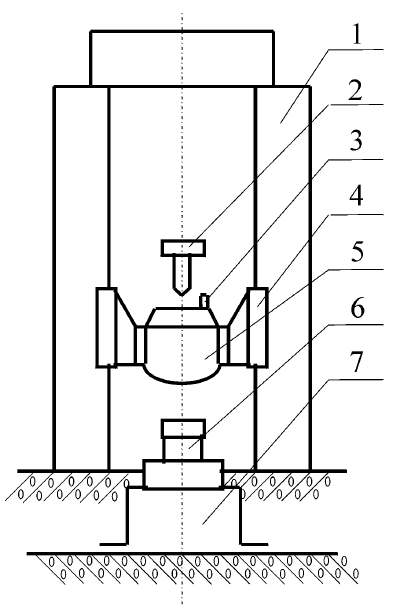
\includegraphics[width=4cm]{cn_100t.png} \\
    1.立柱 2.提升释放机构 3.标准冲击加速度计 \\
    4.导轨 5.重锤 6.被校力传感器 7.底座 \\
  \bicaption[出现在插图索引中]
    {单个图形示例\cite{he1999}。如果表格的标题很长,那么在表格索引中就会很不美观。可
      以在前面用中括号写一个简短的标题,这个标题会出现在索引中。}
    {Stay hungry, stay foolish.}
 \label{fig:cn_100t}
\end{figure}

Lorem ipsum dolor sit amet, consectetur adipisici elit, sed do eiusmod tempor
incididunt ut labore et dolore magna aliqua. Ut enim ad minim veniam, quis
nostrud exercitation ullamco laboris nisi ut aliquip ex ea commodo consequat.
Duis aute irure dolor in reprehenderit in voluptate velit esse cillum dolore eu
fugiat nulla pariatur. Excepteur sint occaecat cupidatat non proident, sunt in
culpa qui officia deserunt mollit anim id est laborum.

\subsection{多个图形}

简单插入多个图形的例子如图~\ref{fig:SRR} 所示。这两个水平并列放置的子图共用一个
图形计数器,没有各自的子图题。

\begin{figure}[!htp]
  \centering
  
\includegraphics[height=2cm]{sjtu-vi-badge-blue.pdf}
  \hspace{1cm}
  
\includegraphics[height=2cm]{sjtu-vi-badge-blue.pdf}
  \bicaption{中文题图}{English caption}
  \label{fig:SRR}
\end{figure}

如果多个图形相互独立,并不共用一个图形计数器,那么用 \texttt{minipage} 或者
\texttt{parbox} 就可以,如图~\ref{fig:parallel1} 与图~\ref{fig:parallel2}。

\begin{figure}[!htp]
\begin{minipage}{0.48\textwidth}
  \centering
  
\includegraphics[height=1.5cm]{sjtu-vi-name-blue.pdf}
  \caption{并排第一个图}
  \label{fig:parallel1}
  \\
  \centering
  
\includegraphics[height=1.5cm]{sjtu-vi-name-blue.pdf}
  \caption{并排第二个图}
  \label{fig:parallel2}
\end{minipage}
\end{figure}

Lorem ipsum dolor sit amet, consectetur adipisici elit, sed do eiusmod tempor
incididunt ut labore et dolore magna aliqua. Ut enim ad minim veniam, quis
nostrud exercitation ullamco laboris nisi ut aliquip ex ea commodo consequat.
Duis aute irure dolor in reprehenderit in voluptate velit esse cillum dolore eu
fugiat nulla pariatur. Excepteur sint occaecat cupidatat non proident, sunt in
culpa qui officia deserunt mollit anim id est laborum.

如果要为共用一个计数器的多个子图添加子图题,建议使用较新的 \pkg{subcaption}宏
包,不建议使用 \pkg{subfigure} 或 \pkg{subfig} 等宏包。

推荐使用 \pkg{subcaption} 宏包的 \cs{subcaptionbox} 并排子图,子图题置于子图之
下,子图号用 a)、b) 等表示。也可以使用 \pkg{subcaption} 宏包的 \cs{subcaption}
(放在 minipage中,用法同 \cs{caption})。

搭配 \pkg{bicaption} 宏包时,可以启用 \cs{subcaptionbox} 和 \cs{subcaption} 的双
语变种 \cs{bisubcaptionbox} 和 \cs{bisubcaption},如图~\ref{fig:bisubcaptionbox}
所示。

\begin{figure}[!hbtp]
  \centering
  \bisubcaptionbox{$R_3 = 1.5\text{mm}$ 时轴承的压力分布云图}%
                  {Pressure contour of bearing when $R_3 = 1.5\text{mm}$}%
                  [6.4cm]{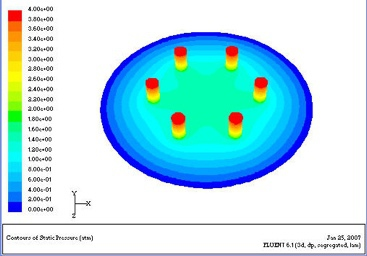
\includegraphics[height=2.5cm]{pressure15.jpg}}
  \hspace{1cm}
  \bisubcaptionbox{$R_3 = 2.5\text{mm}$ 时轴承的压力分布云图}%
                  {Pressure contour of bearing when $R_3 = 2.5\text{mm}$}%
                  [6.4cm]{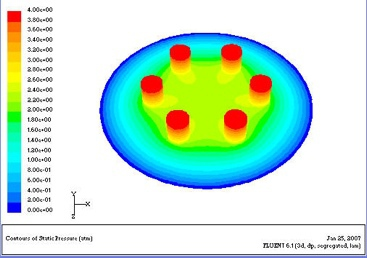
\includegraphics[height=2.5cm]{/pressure25.jpg}}
  \bicaption{包含子图题的范例(使用 subcaptionbox)}
            {Example with subcaptionbox}
  \label{fig:bisubcaptionbox}
\end{figure}

\pkg{subcaption} 宏包也提供了 \pkg{subfigure} 和 \pkg{subtable} 环境,如
图~\ref{fig:subfigure}。

\begin{figure}[!htp]
  \centering
  \begin{subfigure}{0.3\textwidth}
    \centering
    
\includegraphics[height=2cm]{sjtu-vi-badge-blue.pdf}
    \caption{校徽}
  \end{subfigure}
  \hspace{1cm}
  \begin{subfigure}{0.4\textwidth}
    \centering
    
\includegraphics[height=1.5cm]{sjtu-vi-name-blue.pdf}
    \caption{校名。注意这个图略矮些,subfigure 中同一行的子图在顶端对齐。}
  \end{subfigure}
  \caption{包含子图题的范例(使用 subfigure)}
  \label{fig:subfigure}
\end{figure}

Lorem ipsum dolor sit amet, consectetur adipisici elit, sed do eiusmod tempor
incididunt ut labore et dolore magna aliqua. Ut enim ad minim veniam, quis
nostrud exercitation ullamco laboris nisi ut aliquip ex ea commodo consequat.
Duis aute irure dolor in reprehenderit in voluptate velit esse cillum dolore eu
fugiat nulla pariatur. Excepteur sint occaecat cupidatat non proident, sunt in
culpa qui officia deserunt mollit anim id est laborum.

\section{表格}

\subsection{基本表格}

编排表格应简单明了,表达一致,明晰易懂,表文呼应、内容一致。表题置于表上,研究生
学位论文可以用中、英文两种文字居中排写,中文在上,也可以只用中文。

表格的编排建议采用国际通行的三线表\footnote{三线表,以其形式简洁、功能分明、阅读
方便而在科技论文中被推荐使用。三线表通常只有 3 条线,即顶线、底线和栏目线,没有
竖线。}。三线表可以使用 \pkg{booktabs} 提供的 \cs{toprule}、\cs{midrule} 和
\cs{bottomrule}。它们与 \pkg{longtable} 能很好的配合使用。

\begin{table}[!hpt]
  \caption[一个颇为标准的三线表]{一个颇为标准的三线表\footnotemark}
  \label{tab:firstone}
  \centering
  \begin{tabular}{@{}llr@{}} \toprule
    \multicolumn{2}{c}{Item} \\ \cmidrule(r){1-2}
    Animal & Description & Price (\$)\\ \midrule
    Gnat  & per gram  & 13.65 \\
          & each      & 0.01 \\
    Gnu   & stuffed   & 92.50 \\
    Emu   & stuffed   & 33.33 \\
    Armadillo & frozen & 8.99 \\ \bottomrule
  \end{tabular}
\end{table}
\footnotetext{这个例子来自
  \href{https://mirrors.sjtug.sjtu.edu.cn/ctan/macros/latex/contrib/booktabs/booktabs.pdf}%
  {《Publication quality tables in LaTeX》}(\pkg{booktabs} 宏包的文档)。这也是
  一个在表格中使用脚注的例子,请留意与 \pkg{threeparttable} 实现的效果有何不
  同。}

\subsection{复杂表格}

我们经常会在表格下方标注数据来源,或者对表格里面的条目进行解释。可以用
\pkg{threeparttable} 实现带有脚注的表格,如表~\ref{tab:footnote}。

\begin{table}[!htpb]
  \bicaption{一个带有脚注的表格的例子}{A Table with footnotes}
  \label{tab:footnote}
  \centering
  \begin{threeparttable}[b]
     \begin{tabular}{ccd{4}cccc}
      \toprule
      \multirow{2}*{total} & \multicolumn{2}{c}{20\tnote{a}} & \multicolumn{2}{c}{40} & \multicolumn{2}{c}{60} \\
      \cmidrule(lr){2-3}\cmidrule(lr){4-5}\cmidrule(lr){6-7}
      & www & \multicolumn{1}{c}{k} & www & k & www & k \\ % 使用说明符 d 的列会自动进入数学模式,使用 \multicolumn 对文字表头做特殊处理
      \midrule
      & $\underset{(2.12)}{4.22}$ & 120.0140\tnote{b} & 333.15 & 0.0411 & 444.99 & 0.1387 \\
      & 168.6123 & 10.86 & 255.37 & 0.0353 & 376.14 & 0.1058 \\
      & 6.761    & 0.007 & 235.37 & 0.0267 & 348.66 & 0.1010 \\
      \bottomrule
    \end{tabular}
    \begin{tablenotes}
    \item [a] the first note.% or \item [a]
    \item [b] the second note.% or \item [b]
    \end{tablenotes}
  \end{threeparttable}
\end{table}

Lorem ipsum dolor sit amet, consectetur adipisici elit, sed do eiusmod tempor
incididunt ut labore et dolore magna aliqua. Ut enim ad minim veniam, quis
nostrud exercitation ullamco laboris nisi ut aliquip ex ea commodo consequat.
Duis aute irure dolor in reprehenderit in voluptate velit esse cillum dolore eu
fugiat nulla pariatur. Excepteur sint occaecat cupidatat non proident, sunt in
culpa qui officia deserunt mollit anim id est laborum.

如某个表需要转页接排,可以用 \pkg{longtable} 实现。接排时表题省略,表头应重复书
写,并在右上方写“续表 xx”,如表~\ref{tab:performance}。

\begin{longtable}[c]{c*{6}{r}}
  \bicaption{实验数据}{Experimental data}
  \label{tab:performance} \\
  \toprule
  测试程序 & \multicolumn{1}{c}{正常运行} & \multicolumn{1}{c}{同步}
    & \multicolumn{1}{c}{检查点} & \multicolumn{1}{c}{卷回恢复}
    & \multicolumn{1}{c}{进程迁移} & \multicolumn{1}{c}{检查点} \\
   & \multicolumn{1}{c}{时间 (s)} & \multicolumn{1}{c}{时间 (s)}
    & \multicolumn{1}{c}{时间 (s)} & \multicolumn{1}{c}{时间 (s)}
    & \multicolumn{1}{c}{时间 (s)} &  文件(KB)\\
  \midrule
  \endfirsthead
  \multicolumn{7}{r}{续表~\thetable} \\
  \toprule
  测试程序 & \multicolumn{1}{c}{正常运行} & \multicolumn{1}{c}{同步}
    & \multicolumn{1}{c}{检查点} & \multicolumn{1}{c}{卷回恢复}
    & \multicolumn{1}{c}{进程迁移} & \multicolumn{1}{c}{检查点} \\
   & \multicolumn{1}{c}{时间 (s)} & \multicolumn{1}{c}{时间 (s)}
    & \multicolumn{1}{c}{时间 (s)} & \multicolumn{1}{c}{时间 (s)}
    & \multicolumn{1}{c}{时间 (s)}&  文件(KB)\\
  \midrule
  \endhead
  \hline
  \multicolumn{7}{r}{续下页}
  \endfoot
  \endlastfoot
  CG.A.2 & 23.05 & 0.002 & 0.116 & 0.035 & 0.589 & 32491 \\
  CG.A.4 & 15.06 & 0.003 & 0.067 & 0.021 & 0.351 & 18211 \\
  CG.A.8 & 13.38 & 0.004 & 0.072 & 0.023 & 0.210 & 9890 \\
  CG.B.2 & 867.45 & 0.002 & 0.864 & 0.232 & 3.256 & 228562 \\
  CG.B.4 & 501.61 & 0.003 & 0.438 & 0.136 & 2.075 & 123862 \\
  CG.B.8 & 384.65 & 0.004 & 0.457 & 0.108 & 1.235 & 63777 \\
  MG.A.2 & 112.27 & 0.002 & 0.846 & 0.237 & 3.930 & 236473 \\
  MG.A.4 & 59.84 & 0.003 & 0.442 & 0.128 & 2.070 & 123875 \\
  MG.A.8 & 31.38 & 0.003 & 0.476 & 0.114 & 1.041 & 60627 \\
  MG.B.2 & 526.28 & 0.002 & 0.821 & 0.238 & 4.176 & 236635 \\
  MG.B.4 & 280.11 & 0.003 & 0.432 & 0.130 & 1.706 & 123793 \\
  MG.B.8 & 148.29 & 0.003 & 0.442 & 0.116 & 0.893 & 60600 \\
  LU.A.2 & 2116.54 & 0.002 & 0.110 & 0.030 & 0.532 & 28754 \\
  LU.A.4 & 1102.50 & 0.002 & 0.069 & 0.017 & 0.255 & 14915 \\
  LU.A.8 & 574.47 & 0.003 & 0.067 & 0.016 & 0.192 & 8655 \\
  LU.B.2 & 9712.87 & 0.002 & 0.357 & 0.104 & 1.734 & 101975 \\
  LU.B.4 & 4757.80 & 0.003 & 0.190 & 0.056 & 0.808 & 53522 \\
  LU.B.8 & 2444.05 & 0.004 & 0.222 & 0.057 & 0.548 & 30134 \\
  EP.A.2 & 123.81 & 0.002 & 0.010 & 0.003 & 0.074 & 1834 \\
  EP.A.4 & 61.92 & 0.003 & 0.011 & 0.004 & 0.073 & 1743 \\
  EP.A.8 & 31.06 & 0.004 & 0.017 & 0.005 & 0.073 & 1661 \\
  EP.B.2 & 495.49 & 0.001 & 0.009 & 0.003 & 0.196 & 2011 \\
  EP.B.4 & 247.69 & 0.002 & 0.012 & 0.004 & 0.122 & 1663 \\
  EP.B.8 & 126.74 & 0.003 & 0.017 & 0.005 & 0.083 & 1656 \\
  SP.A.2 & 123.81 & 0.002 & 0.010 & 0.003 & 0.074 & 1854 \\
  SP.A.4 & 51.92 & 0.003 & 0.011 & 0.004 & 0.073 & 1543 \\
  SP.A.8 & 31.06 & 0.004 & 0.017 & 0.005 & 0.073 & 1671 \\
  SP.B.2 & 495.49 & 0.001 & 0.009 & 0.003 & 0.196 & 2411 \\
  SP.B.4 & 247.69 & 0.002 & 0.014 & 0.006 & 0.152 & 2653 \\
  SP.B.8 & 126.74 & 0.003 & 0.017 & 0.005 & 0.082 & 1755 \\
  \bottomrule
\end{longtable}

\section{算法环境}

算法环境可以使用 \pkg{algorithms} 宏包或者较新的 \pkg{algorithm2e} 实现。
算法~\ref{algo:algorithm} 是一个使用 \pkg{algorithm2e} 的例子。关于排版算法环境
的具体方法,请阅读相关宏包的官方文档。

\begin{algorithm}[htb]
  \caption{算法示例}
  \label{algo:algorithm}
  \small
  \SetAlgoLined
  \KwData{this text}
  \KwResult{how to write algorithm with \LaTeXe }

  initialization\;
  \While{not at end of this document}{
    read current\;
    \eIf{understand}{
      go to next section\;
      current section becomes this one\;
    }{
      go back to the beginning of current section\;
    }
  }
\end{algorithm}

\section{代码环境}

我们可以在论文中插入算法,但是不建议插入大段的代码。如果确实需要插入代码,建议使
用 \pkg{listings} 宏包。

\begin{codeblock}[language=C]
#include <stdio.h>
#include <unistd.h>
#include <sys/types.h>
#include <sys/wait.h>

int main() {
  pid_t pid;

  switch ((pid = fork())) {
  case -1:
    printf("fork failed\n");
    break;
  case 0:
    /* child calls exec */
    execl("/bin/ls", "ls", "-l", (char*)0);
    printf("execl failed\n");
    break;
  default:
    /* parent uses wait to suspend execution until child finishes */
    wait((int*)0);
    printf("is completed\n");
    break;
  }

  return 0;
}
\end{codeblock}

% % !TEX root = ../main.tex

\chapter{数学与引用文献的标注}

\section{数学}

\subsection{数字和单位}

宏包 \pkg{siunitx} 提供了更好的数字和单位支持:
\begin{itemize}
  \item \num{12345.67890}
  \item \num{1+-2i}
  \item \num{.3e45}
  \item \num{1.654 x 2.34 x 3.430}
  \item \si{kg.m.s^{-1}}
  \item \si{\micro\meter} $\si{\micro\meter}$
  \item \si{\ohm} $\si{\ohm}$
  \item \numlist{10;20}
  \item \numlist{10;20;30}
  \item \SIlist{0.13;0.67;0.80}{\milli\metre}
  \item \numrange{10}{20}
  \item \SIrange{10}{20}{\degreeCelsius}
\end{itemize}

\subsection{数学符号和公式}

微分符号 $\dif$ 应使用正体,本模板提供了 \cs{dif} 命令。除此之外,模板还提供了一
些命令方便使用:
\begin{itemize}
  \item 圆周率 $\uppi$:\verb|\uppi|
  \item 自然对数的底 $\upe$:\verb|\upe|
  \item 虚数单位 $\upi$, $\upj$:\verb|\upi| \verb|\upj|
\end{itemize}

公式应另起一行居中排版。公式后应注明编号,按章顺序编排,编号右端对齐。
\begin{equation}
  \upe^{\upi\uppi} + 1 = 0,
\end{equation}
\begin{equation}
  \frac{\dif^2 u}{\dif t^2} = \int f(x) \dif x.
\end{equation}

公式末尾是需要添加标点符号的,至于用逗号还是句号,取决于公式下面一句是接着公式说的,还是另起一句。
\begin{equation}
		\frac{2h}{\pi}\int_{0}^{\infty}\frac{\sin\left( \omega\delta \right)}{\omega}
		\cos\left( \omega x \right) \dif\omega = 
		\begin{cases}
				h, \ \left| x \right| < \delta, \\
				\frac{h}{2}, \ x = \pm \delta, \\
				0, \ \left| x \right| > \delta.
		\end{cases}
\end{equation}
公式较长时最好在等号“$=$”处转行。
\begin{align}
    & I (X_3; X_4) - I (X_3; X_4 \mid X_1) - I (X_3; X_4 \mid X_2) \nonumber \\
  = & [I (X_3; X_4) - I (X_3; X_4 \mid X_1)] - I (X_3; X_4 \mid \tilde{X}_2) \\
  = & I (X_1; X_3; X_4) - I (X_3; X_4 \mid \tilde{X}_2).
\end{align}

如果在等号处转行难以实现,也可在 $+$、$-$、$\times$、$\div$运算符号处转行,转行
时运算符号仅书写于转行式前,不重复书写。
\begin{multline}
  \frac{1}{2} \Delta (f_{ij} f^{ij}) =
    2 \left(\sum_{i<j} \chi_{ij}(\sigma_{i} - \sigma_{j})^{2}
    + f^{ij} \nabla_{j} \nabla_{i} (\Delta f) \right. \\
  \left. + \nabla_{k} f_{ij} \nabla^{k} f^{ij} +
    f^{ij} f^{k} \left[2\nabla_{i}R_{jk}
    - \nabla_{k} R_{ij} \right] \vphantom{\sum_{i<j}} \right).
\end{multline}

\subsection{定理环境}

示例文件中使用 \pkg{ntheorem} 宏包配置了定理、引理和证明等环境。用户也可以使用
\pkg{amsthm} 宏包。

这里举一个“定理”和“证明”的例子。
\begin{theorem}[留数定理]
\label{thm:res}
  假设 $U$ 是复平面上的一个单连通开子集,$a_1, \ldots, a_n$ 是复平面上有限个点,
  $f$ 是定义在 $U \backslash \{a_1, \ldots, a_n\}$ 上的全纯函数,如果 $\gamma$
  是一条把 $a_1, \ldots, a_n$ 包围起来的可求长曲线,但不经过任何一个 $a_k$,并且
  其起点与终点重合,那么:

  \begin{equation}
    \label{eq:res}
    \ointop_\gamma f(z)\, \dif z = 2\uppi \upi \sum_{k=1}^n \operatorname{I}(\gamma, a_k) \operatorname{Res}(f, a_k).
  \end{equation}

  如果 $\gamma$ 是若尔当曲线,那么 $\operatorname{I}(\gamma, a_k) = 1$,因此:

  \begin{equation}
    \label{eq:resthm}
    \ointop_\gamma f(z)\, \dif z = 2\uppi \upi \sum_{k=1}^n \operatorname{Res}(f, a_k).
  \end{equation}

  在这里,$\operatorname{Res}(f, a_k)$ 表示 $f$ 在点 $a_k$ 的留数,
  $\operatorname{I}(\gamma, a_k)$ 表示 $\gamma$ 关于点 $a_k$ 的卷绕数。卷绕数是
  一个整数,它描述了曲线 $\gamma$ 绕过点 $a_k$ 的次数。如果 $\gamma$ 依逆时针方
  向绕着 $a_k$ 移动,卷绕数就是一个正数,如果 $\gamma$ 根本不绕过 $a_k$,卷绕数
  就是零。

  定理~\ref{thm:res} 的证明。

  \begin{proof}
    首先,由……

    其次,……

    所以……
  \end{proof}
\end{theorem}

\section{引用文献的标注}

按照教务处的要求,参考文献外观应符合国标 GB/T 7714 的要求。模版使用 \BibLaTeX\
配合 \pkg{biblatex-gb7714-2015} 样式包
\footnote{\url{https://www.ctan.org/pkg/biblatex-gb7714-2015}}
控制参考文献的输出样式,后端采用 \pkg{biber} 管理文献。

请注意 \pkg{biblatex-gb7714-2015} 宏包 2016 年 9 月才加入 CTAN,如果你使用的
\TeX\ 系统版本较旧,可能没有包含 \pkg{biblatex-gb7714-2015} 宏包,需要手动安装。
\BibLaTeX\ 与 \pkg{biblatex-gb7714-2015} 目前在活跃地更新,为避免一些兼容性问
题,推荐使用较新的版本。

正文中引用参考文献时,使用 \verb|\cite{key1,key2,key3...}| 可以产生“上标引用的
参考文献”,如 \cite{Meta_CN,chen2007act,DPMG}。使用
\verb|\parencite{key1,key2,key3...}| 则可以产生水平引用的参考文献,例如
\parencite{JohnD,zhubajie,IEEE-1363}。请看下面的例子,将会穿插使用水平的和上标的
参考文献:关于书的\parencite{Meta_CN,JohnD,IEEE-1363},关于期刊的
\cite{chen2007act,chen2007ewi},会议论文 \parencite{DPMG,kocher99,cnproceed},硕
士学位论文\parencite{zhubajie,metamori2004},博士学位论文
\cite{shaheshang,FistSystem01,bai2008},标准文件 \parencite{IEEE-1363},技术报告
\cite{NPB2},电子文献 \parencite{xiaoyu2001, CHRISTINE1998},用户手册
\parencite{RManual}。

当需要将参考文献条目加入到文献表中但又不在正文中引用,可以使用
\verb|\nocite{key1,key2,key3...}|。使用 \verb|\nocite{*}| 可以将参考文献数据库中
的所有条目加入到文献表中。

% % !TEX root = ../thesis.tex

\begin{summary}
这里是全文总结内容。

2015 年 2 月 28 日,中央在北京召开全国精神文明建设工作表彰暨学雷锋志愿服务大会,
公布全国文明城市(区)、文明村镇、文明单位名单。上海交通大学荣获全国文明单位称
号。

全国文明单位这一荣誉是对交大人始终高度重视文明文化工作的肯定,是对交大长期以来文
明创建工作成绩的褒奖。在学校党委、文明委的领导下,交大坚持将文明创建工作纳入学校
建设世界一流大学的工作中,全体师生医护员工群策群力、积极开拓,落实国家和上海市有
关文明创建的各项要求,以改革创新、科学发展为主线,以质量提升为目标,聚焦文明创建
工作出现的重点和难点,优化文明创建工作机制,传播学校良好形象,提升社会美誉度,显
著增强学校软实力。2007 至 2012 年间,上海交大连续三届荣获“上海市文明单位”称
号,成为创建全国文明单位的新起点。

上海交大自启动争创全国文明单位工作以来,凝魂聚气、改革创新,积极培育和践行社会主
义核心价值观。坚持统筹兼顾、多措并举,将争创全国文明单位与学校各项中心工作紧密结
合,着力构建学校文明创建新格局,不断提升师生医护员工文明素养,以“冲击世界一流大
学汇聚强大精神动力”为指导思想,以“聚焦改革、多元推进、以评促建、丰富内涵、彰显
特色”为工作原则,并由全体校领导群策领衔“党的建设深化、思想教育深入、办学成绩显
著、大学文化丰富、校园环境优化、社会责任担当”六大板块共 28 项重点突破工作,全面
展现近年来交大文明创建工作的全貌和成就。

进入新阶段,学校将继续开拓文明创建工作新格局,不断深化工作理念和工作实践,创新工
作载体、丰富活动内涵、凸显创建成效,积极服务于学校各项中心工作和改革发展的大局
面,在上级党委、文明委的关心下,在学校党委的直接领导下,与时俱进、开拓创新,为深
化内涵建设、加快建成世界一流大学、推动国家进步和社会发展而努力奋斗!

上海交通大学医学院附属仁济医院也获得全国文明单位称号。
\end{summary}



% 使用英文字母对附录编号
\appendix

% 附录内容,本科学位论文可以用翻译的文献替代。

% % !TEX root = ../thesis.tex

\chapter{Maxwell Equations}

选择二维情况,有如下的偏振矢量:
\begin{subequations}
  \begin{align}
    {\bf E} &= E_z(r, \theta) \hat{\bf z}, \\
    {\bf H} &= H_r(r, \theta) \hat{\bf r} + H_\theta(r, \theta) \hat{\bm\theta}.
  \end{align}
\end{subequations}
对上式求旋度:
\begin{subequations}
  \begin{align}
    \nabla \times {\bf E} &= \frac{1}{r} \frac{\partial E_z}{\partial\theta}
      \hat{\bf r} - \frac{\partial E_z}{\partial r} \hat{\bm\theta}, \\
    \nabla \times {\bf H} &= \left[\frac{1}{r} \frac{\partial}{\partial r}
      (r H_\theta) - \frac{1}{r} \frac{\partial H_r}{\partial\theta} \right]
      \hat{\bf z}.
  \end{align}
\end{subequations}
因为在柱坐标系下,$\overline{\overline\mu}$ 是对角的,所以 Maxwell 方程组中电场
$\bf E$ 的旋度:
\begin{subequations}
  \begin{align}
    & \nabla \times {\bf E} = \upi \omega {\bf B}, \\
    & \frac{1}{r} \frac{\partial E_z}{\partial\theta} \hat{\bf r} -
      \frac{\partial E_z}{\partial r}\hat{\bm\theta} = \upi \omega \mu_r H_r
      \hat{\bf r} + \upi \omega \mu_\theta H_\theta \hat{\bm\theta}.
  \end{align}
\end{subequations}
所以 $\bf H$ 的各个分量可以写为:
\begin{subequations}
  \begin{align}
    H_r &= \frac{1}{\upi \omega \mu_r} \frac{1}{r}
      \frac{\partial E_z}{\partial\theta}, \\
    H_\theta &= -\frac{1}{\upi \omega \mu_\theta}
      \frac{\partial E_z}{\partial r}.
  \end{align}
\end{subequations}
同样地,在柱坐标系下,$\overline{\overline\epsilon}$ 是对角的,所以 Maxwell 方程
组中磁场 $\bf H$ 的旋度:
\begin{subequations}
  \begin{align}
    & \nabla \times {\bf H} = -\upi \omega {\bf D}, \\
    & \left[\frac{1}{r} \frac{\partial}{\partial r}(r H_\theta) - \frac{1}{r}
      \frac{\partial H_r}{\partial\theta} \right] \hat{\bf z} = -\upi \omega
      {\overline{\overline\epsilon}} {\bf E} = -\upi \omega \epsilon_z E_z
      \hat{\bf z}, \\
    & \frac{1}{r} \frac{\partial}{\partial r}(r H_\theta) - \frac{1}{r}
      \frac{\partial H_r}{\partial\theta} = -\upi \omega \epsilon_z E_z.
  \end{align}
\end{subequations}
由此我们可以得到关于 $E_z$ 的波函数方程:
\begin{equation}
  \frac{1}{\mu_\theta \epsilon_z} \frac{1}{r} \frac{\partial}{\partial r}
  \left(r \frac{\partial E_z}{\partial r} \right) + \frac{1}{\mu_r \epsilon_z}
  \frac{1}{r^2} \frac{\partial^2E_z}{\partial\theta^2} +\omega^2 E_z = 0.
\end{equation}

% % !TEX root = ../thesis.tex

\chapter{绘制流程图}

图~\ref{fig:flow_chart} 是一张流程图示意。使用 \pkg{tikz} 环境,搭配四种预定义节
点(\verb+startstop+、\verb+process+、\verb+decision+和\verb+io+),可以容易地绘
制出流程图。

\begin{figure}[!htp]
  \centering
  \resizebox{6cm}{!}{\begin{tikzpicture}[node distance=2cm]
    \node (pic) [startstop] {待测图片};
    \node (bg) [io, below of=pic] {读取背景};
    \node (pair) [process, below of=bg] {匹配特征点对};
    \node (threshold) [decision, below of=pair, yshift=-0.5cm] {多于阈值};
    \node (clear) [decision, right of=threshold, xshift=3cm] {清晰?};
    \node (capture) [process, right of=pair, xshift=3cm, yshift=0.5cm] {重采};
    \node (matrix_p) [process, below of=threshold, yshift=-0.8cm] {透视变换矩阵};
    \node (matrix_a) [process, right of=matrix_p, xshift=3cm] {仿射变换矩阵};
    \node (reg) [process, below of=matrix_p] {图像修正};
    \node (return) [startstop, below of=reg] {配准结果};
     
    %连接具体形状
    \draw [arrow](pic) -- (bg);
    \draw [arrow](bg) -- (pair);
    \draw [arrow](pair) -- (threshold);

    \draw [arrow](threshold) -- node[anchor=south] {否} (clear);

    \draw [arrow](clear) -- node[anchor=west] {否} (capture);
    \draw [arrow](capture) |- (pic);
    \draw [arrow](clear) -- node[anchor=west] {是} (matrix_a);
    \draw [arrow](matrix_a) |- (reg);

    \draw [arrow](threshold) -- node[anchor=east] {是} (matrix_p);
    \draw [arrow](matrix_p) -- (reg);
    \draw [arrow](reg) -- (return);
\end{tikzpicture}
}
  \bicaption{绘制流程图效果}{Flow chart}
  \label{fig:flow_chart}
\end{figure}

% !TeX root = ../thesis.tex
\chapter{Gossip-Style Membership协议的Go语言实现}\label{app:code}
\begin{codeblock}[language=GO]
    package simple

import (
	"fmt"
	"math/rand"
	"time"
)

const (
	P_FAIL=0.1
	GOSSIP_INTERVAL=time.Second //1s发一次
	REPAIR_TIME=4*time.Second
	NODE_NUM = 6
	BUFSIZE = 5 //channel buffer size 一般设置为数据中心节点的数目即可
	K = 2
	IS_AUTO = true
)

type Nil struct {}

type Node struct {
	isbad bool
	trans chan []Message
	time chan Nil
	timeout chan Nil
	accept chan []Message
	deliver chan []Message
	Others []*Node
	//仅打日志及图形化显示使用
	address string
	membership *Membership
}

func NewNode(address string) (instance *Node) {
	instance = new(Node)
	instance.accept = make(chan []Message)
	instance.deliver = make(chan []Message)
	instance.trans = make(chan []Message, BUFSIZE)
	instance.time = make(chan Nil)
	instance.timeout = make(chan Nil)
	instance.isbad = false
	instance.address = address
	instance.Others = make([]*Node, 0)
	instance.membership = NewMembership(address, instance.accept, instance.deliver)
	fmt.Printf("Initialized Node %p\n", instance)
	return
}

//多路复用实现Nondeterminated Choice
func (node *Node) Fragile() {
	fmt.Printf("Node %p Starts\n", node)
	go node.timer()
	go node.membership.Running()
	node.time <- Nil{}
	for {
		if (IS_AUTO) {
			node.Bad()
		}
		if (node.isbad) {
			time.Sleep(REPAIR_TIME)
			continue
		}
		select {
		case message := <- node.trans:
			node.deliver <- message
			for len(node.trans) > 0 {
				message = <- node.trans
				node.deliver <- message
			}
		case <- node.timeout:
			messages := <- node.accept
			node.Gossiping(messages)
		}
	}
}
func (node *Node) Bad() {
	rand.Seed(time.Now().UnixNano())
		r := rand.Float32()
		if r < P_FAIL {
			node.isbad = true
		} else {
			node.isbad = false
		}
}
func (node *Node) timer() {
	for {
		select {
		case <- node.time:
			time.Sleep(GOSSIP_INTERVAL)
			node.timeout <- Nil{}
		}
	}
}

func (node *Node) Gossiping(messages []Message) {
	rand.Seed(time.Now().UnixNano())
	//随机全排列,取前K个
	perm := rand.Perm(len(node.Others))[:K]
	var targets []*Node
	for _, p := range perm {
		targets = append(targets, node.Others[p])
	}
	str := transmitting(messages, targets)
	fmt.Printf("[SEND] From: %s; To: %s\n", node.address, str)
	node.time <- Nil{}
}

func transmitting(messages []Message, targets []*Node) string {
	var str string
	for _, t := range targets {
		if (len(t.trans) == BUFSIZE) {
			continue
		}
		t.trans <- messages
		str+=(t.address+" ")
	}
	return str
}

func (node *Node)ChangeStatus() {
	node.isbad = !node.isbad
}

func (node *Node)Address() string {
	return node.address
}
\end{codeblock}

\begin{codeblock}[language=GO]
    package simple

import (
	"time"
	"fmt"
)

type Message struct {
	Address string
	Heartbeat int
}

type Cell struct {
	Message Message
	LocalTime int64
}

type Membership struct {
	address string
	heartbeat int
	membershipList map[string]Cell
	accept chan []Message
	deliver chan []Message
}

func NewMembership(address string, accept chan []Message, deliver chan[]Message) (instance *Membership){
	instance = new(Membership)
	instance.address = address
	instance.heartbeat = 0
	instance.membershipList = make(map[string]Cell,0)
	instance.accept = accept
	instance.deliver = deliver
	fmt.Printf("Initialzed Membership %p\n", instance)
	return
}

func (membership *Membership) Running() {
	for {
		select {
		case messages := <- membership.deliver:
			membership.Deliver(messages)
		case membership.accept <- membership.Accept():

		}
	}
}

func (membership *Membership) Deliver(messages []Message) {
	list := membership.membershipList
	for _, message := range messages {
		if message.Address == membership.address {
			continue
		}
		if cell, ok := list[message.Address]; !ok || (cell.Message.Heartbeat < message.Heartbeat) {
			//MembershipList中没有这个节点的信息或信息是旧的,增加或更新
			list[message.Address] = Cell{Message:Copy(message), LocalTime:time.Now().UnixNano()}
		} 
	}
	membership.PrintUpdate()
}

func (membership *Membership) Accept() (messages []Message) {
	list := membership.membershipList
	messages = make([]Message, 0)
	membership.heartbeat++
	messages = append(messages, Message{membership.address, membership.heartbeat})
	for _, cell := range list {
		messages = append(messages, Copy(cell.Message))
	}
	return
}
\end{codeblock}
\begin{codeblock}[language=GO]
    package main

import (
	"encoding/json"
	"fmt"
    "./simple"
    "strconv"
    "log"
    "net/http"
    "io/ioutil"
)

var nodes []*simple.Node

func main() {
    nodes = make([]*simple.Node, 0)
    for i:=0;i<simple.NODE_NUM;i++ {
        nodes = append(nodes, simple.NewNode("address"+strconv.Itoa(i)))
    }

    for i:=0;i<simple.NODE_NUM;i++ {
        nodes[i].Others = append(nodes[i].Others, nodes[:i]...)
        nodes[i].Others = append(nodes[i].Others, nodes[i+1:]...)
        go nodes[i].Fragile()
    }

    for {
        http.HandleFunc("/index", index)
        http.HandleFunc("/membership", membership)
        http.HandleFunc("/change_status", changeStatus)
        log.Fatal(http.ListenAndServe("localhost:8080", nil))
    }
}

func index(w http.ResponseWriter, r *http.Request) {
    body, _ := ioutil.ReadFile("templates/index.html")
    fmt.Fprint(w, string(body))
}

func membership(w http.ResponseWriter, r *http.Request) {
    header := w.Header()
    header.Add("Content-Type","application/json")
    w.WriteHeader(http.StatusOK)
    var s []simple.Info
    for _, node := range nodes {
        s = append(s, node.Info())
    }
    b, err := json.Marshal(s)
    if err!= nil {
        log.Println("marshal error")
    }
    fmt.Fprintf(w, string(b))
}

func changeStatus(w http.ResponseWriter, r *http.Request) {
    vars := r.URL.Query() 
    address := vars["address"][0]
    for _, node := range nodes {
        if (node.Address() == address) {
            node.ChangeStatus()
        }
    }
    header := w.Header()
    header.Add("Content-Type","application/json")
    w.WriteHeader(http.StatusOK)
}


\end{codeblock}

% 文后无编号部分
\backmatter

% 参考资料
\printbibliography[heading=bibintoc]

% 用于盲审的论文需隐去致谢、发表论文、参与项目、申请专利、简历

% 致谢
% !TEX root = ../main.tex

\begin{acknowledgements}
  感谢那位最先制作出博士学位论文 \LaTeX 模板的交大物理系同学!

  感谢 William Wang 同学对模板移植做出的巨大贡献!

  感谢 \href{https://github.com/weijianwen}{@weijianwen} 学长一直以来的开发和维
  护工作!

  感谢 \href{https://github.com/sjtug}{@sjtug} 以及
   \href{https://github.com/dyweb}{@dyweb} 对 0.9.5 之后版本的开发和维护工作!

  感谢所有为模板贡献过代码的同学们, 以及所有测试和使用模板的各位同学!

  感谢 \LaTeX 和 \href{https://github.com/sjtug/SJTUThesis}{\sjtuthesis},帮我节
  省了不少时间。
\end{acknowledgements}


% 发表论文、参与项目、申请专利、简历
% 盲审论文中,发表学术论文及参与科研情况等仅以第几作者注明即可,不要出现作者或他人姓名
% % !TEX root = ../main.tex

\begin{publications}
  \item Chen H, Chan C~T. Acoustic cloaking in three dimensions using acoustic metamaterials[J]. Applied Physics Letters, 2007, 91:183518.
  \item Chen H, Wu B~I, Zhang B, et al. Electromagnetic Wave Interactions with a Metamaterial Cloak[J]. Physical Review Letters, 2007, 99(6):63903.
\end{publications}

\begin{publications*}
  \item 第一作者. 中文核心期刊论文, 2007.
  \item 第一作者. EI 国际会议论文, 2006.
\end{publications*}

% % !TEX root = ../main.tex

\begin{achievements}
  \item 第一发明人,“永动机”,专利申请号202510149890.0
\end{achievements}

\begin{achievements*}
  \item 第一发明人,“永动机”,专利申请号XXXXXXXXXXXX.X
\end{achievements*}

% % !TEX root = ../main.tex

\begin{resume}
  \subsection*{基本情况}
    某某,yyyy 年 mm 月生于 xxxx。

  \subsection*{教育背景}
  \begin{itemize}
    \item yyyy 年 mm 月至今,上海交通大学,博士研究生,xx 专业
    \item yyyy 年 mm 月至 yyyy 年 mm 月,上海交通大学,硕士研究生,xx 专业
    \item yyyy 年 mm 月至 yyyy 年 mm 月,上海交通大学,本科,xx 专业
  \end{itemize}

  \subsection*{研究兴趣}
    \LaTeX{} 排版

  \subsection*{联系方式}
  \begin{itemize}
    \item 地址: 上海市闵行区东川路 800 号,200240
    \item E-mail: \email{xxx@sjtu.edu.cn}
  \end{itemize}
\end{resume}


% 中文学士学位论文要求在最后有一个英文大摘要,单独编页码,英文学士学位论文不需要
% !TEX root = ../main.tex

\begin{digest}
<<<<<<< HEAD
  With the rapid development of parallel and distributed computer system, concurrency theory has become an important branch of the theory of programs. Research on concurrency theory deepens people’s understanding of concurrent system. Some of the research outcomes have already been used in mainstream programming languages with concurrency features, like Ada and Java. Process calculus is a kind of formal methods using algebraic methods to study concurrent system, such as CCS, CSP and ACP. As a model for describing concurrent systems, process calculus has been extensively studied and successfully applied to the specification, design, analysis, and verification of actual systems.
  
  Modern computer systems, which are open, distributed and interactive, have both nondeterministic behaviors and random choices. In order to use simple, easy-to-use formal methods to describe complex concurrent systems, and to model and analyze concurrent systems, we usually use statistical behavioral characteristics of non-deterministic behavior. Therefore, it is meaningful to introduce the concept of randomness in the concurrent process model. As an important extant to concurrency theory, probabilistic process has been widely researched. Recently, Fu proposes a Uniform Approach used to turn a process model into a randomized extension. Since it is a model independent approach, we can use it to derive a probabilistic extension of any other process model. Fu expresses Uniform Approach by demonstrating how to define the grammar and syntax of RCCS, a randomized version of CCS, and provides us a way to define bisimulation and equivalence on RCCS as well.

  A value-passing calculus is a process calculus where the content of communications are values chosen from some data domain, and the propositions appearing in the conditionals are formulas constructed from a logic. It can be applied to modeling and analyzing communicating processes, biological processes and other real-world problems with value-passing characteristics. In most studies of value-passing calculus, there exits some oracles providing data domain, logic decision and even computation of functions in value-passing processes. Those oracles are usually remained undefined making it hard to analyze the expressiveness of those models. However, Fu proposes a value-passing calculus, called $\mathbb{VPC}_{\mathsf{Th}}$, using a first order theory to decide the bool expression and a turing complete numeric system to derive the outcomes of functions, which successfully avoid such oracles. 
  
  Consider $\mathbb{VPC}_{\mathsf{Th}}$’s great expressiveness, we decide to use Uniform Approach to extend $\mathbb{VPC}_{\mathsf{Th}}$ into a probabilistic version, called $\mathbb{RVPC}_{\mathsf{Th}}$. Hopefully, $\mathbb{RVPC}_{\mathsf{Th}}$ could help to model and analyze some meaningful real-world process such as communication and network security etc. With the aim of benefit mankind, we apply Uniform Approach to $\mathbb{VPC}_{\mathsf{Th}}$ and get the grammar and symbolic transition syntax of $\mathbb{RVPC}_{\mathsf{Th}}$, specifically, we add random choice operator to $\mathbb{RVPC}_{\mathsf{Th}}$ as well as a transition rule to random choice. 
  
  Equivalence of processes is a basic topic of the theory of programs. In the field of process calculus, we usually use bisimulation to describe the equivalence of process models. Bisimulation has been studied for many years since process calculus came into being. Representative work includes Milner’s weak bisimulation and van Glabbeek and Weijland’s branching bisimulation. As for equivalence of probabilistic process, there already exits some research on full probabilistic processes, finite states probabilistic processes etc. However, it is hard to use branching bisimulation or weak bisimulation to describe the equivalence of value-passing process because of the conditional operator. In this way, scholars came up with a symbolic bisimulation for value-passing calculus. Fu also defined the symbolic bisimulation of $\mathbb{VPC}_{\mathsf{Th}}$. 
  
  Uniform Approach proposes a random version of branching bisimulation to describe the equivalence of RCCS. Similarly, we can use the method in Uniform Approach to define a random version of symbolic bisimulation for our $\mathbb{RVPC}_{\mathsf{Th}}$. The core idea to derive a random version of a certain bisimulation is to find out a random version of state-preserving silent transition. Uniform Approach uses Epsilon tree to construct a random branching bisimulation. The main difficulty of using Uniform Approach to define $\mathbb{RVPC}_{\mathsf{Th}}$’s symbolic bisimulation is still the conditional operator. With the aim of eliminate the influence of conditional operator, we propose the conditional equivalence class and conditional Epsilon tree. After defining the conditional l-transition and q-transition, we propose a random symbolic bisimulation. The essence of our symbolic bisimulation is that we can find a division of a certain condition and use conditional epsilon trees corresponding to each element in the division to simulate a conditional epsilon tree. As for some special processes that have a conditional epsilon tree with all branches infinite, we define the codivergence of $\mathbb{RVPC}_{\mathsf{Th}}$ for those processes. Then we define the observance equivalence of $\mathbb{RVPC}_{\mathsf{Th}}$ as the largest codivergent and symbolic bisimulating relation. We manage to prove the congruence of our observance equivalence. Meanwhile, we also provide some interesting examples to annotate the concepts mentioned above.
  
  In addition, for showing our newly proposed random value-passing process model is feasible to model and analyze some real-world processes, we decide to model a real-world process as a demo. Since gossip protocol is interesting, widely known and easy to understand and failure detection is a mainstream topic of cloud computing, we choose to model and analyze a communicating process based on a failure detection mechanism, Gossip-Style Membership Protocol. There’s something with randomization inside gossip protocol that every gossip time, each node will pick k other nodes in a cluster to send gossip message. It is a good property for us to apply our random value-passing process model. We firstly construct a peer-to-peer system where nodes all use gossip protocol to communicate with each other. Since gossip is used to implement multicast in a group, we also define a specification of a multicasting system and prove that the multicasting system is symbolic bisimulated with our peer-to-peer system based on gossip protocol. Next, we adjust the definition of the former peer-to-peer system and using $\mathbb{RVPC}_{\mathsf{Th}}$ to define a membership system interacting with nodes connected to the communicating network of the peer-to-peer system. Finally, we use Golang to implement our peer-to-peer system and use html and javascript to show the result. Result shows that our peer-to-peer system implemented using $\mathbb{RVPC}_{\mathsf{Th}}$ runs correctly, which implies that $\mathbb{RVPC}_{\mathsf{Th}}$ is feasible to be used in modeling and analyzing real-world process with value-passing characteristics, such as communicating processes and biology processes etc. Hopefully, after we define and prove several concepts of $\mathbb{RVPC}_{\mathsf{Th}}$ and demonstrate with an application of it, modeling and analyzing real-world process with value-passing characteristics could be easier and even a routine work.

  Although there still exists something not well considered in our model, our expansion of the value-passing process model, for one hand, further supports the model independence of the Uniform Approach. On the one hand, it proves the feasibility of applying the random value-passing process model to the modeling and analysis of concurrent systems with value-passing characteristics.

\end{digest}


\end{document}
